
\documentclass[a4paper,11pt,twoside]{ThesisStyle}

%\usepackage{graphicx}


\usepackage{fancyvrb}
\usepackage{amsmath}
\usepackage{amssymb}
\usepackage{mathrsfs}
\bibliographystyle{unsrt}
\usepackage{url}
\usepackage{listings}
\usepackage{tabularx}
\usepackage{pdflscape}
%\usepackage{subfigure}
\usepackage{wrapfig,lipsum,booktabs}
\usepackage{multirow}
\usepackage{booktabs}
\usepackage{algorithm}
\usepackage{algorithmic}
\usepackage{gensymb}
\usepackage{pifont}

\newtheorem{deflda}{Axiom}
\newcommand{\ghis}[1]{\noindent\textcolor{blue}{{\bf \{Ghis}: #1{\bf \}}}}
\newcommand{\geom}{\textsc{GeomRDF}\xspace}
\newcommand{\geolift}{\textsc{GeoLift}\xspace}
\newcommand{\limes}{\textsc{Limes}\xspace}


\usepackage{amsmath,amssymb}             % AMS Math
% \usepackage[french]{babel}
\usepackage[latin1]{inputenc}
\usepackage[T1]{fontenc}
\usepackage[left=1.5in,right=1.3in,top=1.1in,bottom=1.1in,includefoot,includehead,headheight=13.6pt]{geometry}
\renewcommand{\baselinestretch}{1.05}

% Table of contents for each chapter

\usepackage[nottoc, notlof, notlot]{tocbibind}
\usepackage{minitoc}
\setcounter{minitocdepth}{2}
\mtcindent=15pt
% Use \minitoc where tos put a table of contents

\usepackage{aecompl}

% Glossary / list of abbreviations

\usepackage[intoc]{nomencl}
\renewcommand{\nomname}{List of Abbreviations}

\makenomenclature

% My pdf code

\usepackage{ifpdf}

\ifpdf
  \usepackage[pdftex]{graphicx}
  \DeclareGraphicsExtensions{.jpg}
  \usepackage[a4paper,pagebackref,hyperindex=true]{hyperref}
\else
  \usepackage{graphicx}
  \DeclareGraphicsExtensions{.ps,.eps}
  \usepackage[a4paper,dvipdfm,pagebackref,hyperindex=true]{hyperref}
\fi

\graphicspath{{.}{images/}}

% Links in pdf
\usepackage{color}
\definecolor{linkcol}{rgb}{0,0,0.4} 
\definecolor{citecol}{rgb}{0.5,0,0} 

% Change this to change the informations included in the pdf file

% See hyperref documentation for information on those parameters

\hypersetup
{
bookmarksopen=true,
pdftitle="First class futures",
pdfauthor="Muhammad Uzair KHAN", 
pdfsubject="update strategies for first class futures", %subject of the document
%pdftoolbar=false, % toolbar hidden
pdfmenubar=true, %menubar shown
pdfhighlight=/O, %effect of clicking on a link
colorlinks=true, %couleurs sur les liens hypertextes
pdfpagemode=None, %aucun mode de page
pdfpagelayout=SinglePage, %ouverture en simple page
pdffitwindow=true, %pages ouvertes entierement dans toute la fenetre
linkcolor=linkcol, %couleur des liens hypertextes internes
citecolor=citecol, %couleur des liens pour les citations
urlcolor=linkcol %couleur des liens pour les url
}

% definitions.
% -------------------

\setcounter{secnumdepth}{3}
\setcounter{tocdepth}{2}

% Some useful commands and shortcut for maths:  partial derivative and stuff

\usepackage [table]{xcolor}


\newcommand{\pd}[2]{\frac{\partial #1}{\partial #2}}
\def\abs{\operatorname{abs}}
\def\argmax{\operatornamewithlimits{arg\,max}}
\def\argmin{\operatornamewithlimits{arg\,min}}
\def\diag{\operatorname{Diag}}
\newcommand{\eqRef}[1]{(\ref{#1})}

\usepackage{rotating}                    % Sideways of figures & tables
%\usepackage{bibunits}
%\usepackage[sectionbib]{chapterbib}          % Cross-reference package (Natural BiB)
%\usepackage{natbib}                  % Put References at the end of each chapter
                                         % Do not put 'sectionbib' option here.
                                         % Sectionbib option in 'natbib' will do.
\usepackage{fancyhdr}                    % Fancy Header and Footer

% \usepackage{txfonts}                     % Public Times New Roman text & math font
  
%%% Fancy Header %%%%%%%%%%%%%%%%%%%%%%%%%%%%%%%%%%%%%%%%%%%%%%%%%%%%%%%%%%%%%%%%%%
% Fancy Header Style Options

\pagestyle{fancy}                       % Sets fancy header and footer
\fancyfoot{}                            % Delete current footer settings

%\renewcommand{\chaptermark}[1]{         % Lower Case Chapter marker style
%  \markboth{\chaptername\ \thechapter.\ #1}}{}} %

%\renewcommand{\sectionmark}[1]{         % Lower case Section marker style
%  \markright{\thesection.\ #1}}         %

\fancyhead[LE,RO]{\bfseries\thepage}    % Page number (boldface) in left on even
% pages and right on odd pages
\fancyhead[RE]{\bfseries\nouppercase{\leftmark}}      % Chapter in the right on even pages
\fancyhead[LO]{\bfseries\nouppercase{\rightmark}}     % Section in the left on odd pages

\let\headruleORIG\headrule
\renewcommand{\headrule}{\color{black} \headruleORIG}
\renewcommand{\headrulewidth}{1.0pt}
\usepackage{colortbl}
\arrayrulecolor{black}

\fancypagestyle{plain}{
  \fancyhead{}
  \fancyfoot{}
  \renewcommand{\headrulewidth}{0pt}
}

%\usepackage{algorithm}
%\usepackage{algorithmic}
%\usepackage[ruled,vlined]{algorithm2e}
%%% Clear Header %%%%%%%%%%%%%%%%%%%%%%%%%%%%%%%%%%%%%%%%%%%%%%%%%%%%%%%%%%%%%%%%%%
% Clear Header Style on the Last Empty Odd pages
\makeatletter

\def\cleardoublepage{\clearpage\if@twoside \ifodd\c@page\else%
  \hbox{}%
  \thispagestyle{empty}%              % Empty header styles
  \newpage%
  \if@twocolumn\hbox{}\newpage\fi\fi\fi}

\makeatother
 
%%%%%%%%%%%%%%%%%%%%%%%%%%%%%%%%%%%%%%%%%%%%%%%%%%%%%%%%%%%%%%%%%%%%%%%%%%%%%%% 
% Prints your review date and 'Draft Version' (From Josullvn, CS, CMU)
\newcommand{\reviewtimetoday}[2]{\special{!userdict begin
    /bop-hook{gsave 20 710 translate 45 rotate 0.8 setgray
      /Times-Roman findfont 12 scalefont setfont 0 0   moveto (#1) show
      0 -12 moveto (#2) show grestore}def end}}
% You can turn on or off this option.
% \reviewtimetoday{\today}{Draft Version}
%%%%%%%%%%%%%%%%%%%%%%%%%%%%%%%%%%%%%%%%%%%%%%%%%%%%%%%%%%%%%%%%%%%%%%%%%%%%%%% 

\newenvironment{maxime}[1]
{
\vspace*{0cm}
\hfill
\begin{minipage}{0.5\textwidth}%
%\rule[0.5ex]{\textwidth}{0.1mm}\\%
\hrulefill $\:$ {\bf #1}\\
%\vspace*{-0.25cm}
\it 
}%
{%

\hrulefill
\vspace*{0.5cm}%
\end{minipage}
}

\let\minitocORIG\minitoc
\renewcommand{\minitoc}{\minitocORIG \vspace{1.5em}}

\usepackage{multirow}
%\usepackage{slashbox}

\newenvironment{bulletList}%
{ \begin{list}%
	{$\bullet$}%
	{\setlength{\labelwidth}{25pt}%
	 \setlength{\leftmargin}{30pt}%
	 \setlength{\itemsep}{\parsep}}}%
{ \end{list} }

\newtheorem{definition}{D�finition}
\renewcommand{\epsilon}{\varepsilon}

% centered page environment

\newenvironment{vcenterpage}
{\newpage\vspace*{\fill}\thispagestyle{empty}\renewcommand{\headrulewidth}{0pt}}
{\vspace*{\fill}}
\usepackage{verbatim}
%\usepackage{minitoc}
%\usepackage{wrapfig}
\usepackage{listings}
\usepackage{hyperref}
\hypersetup{
    bookmarks=true,         % show bookmarks bar?
    unicode=false,          % non-Latin characters in Acrobat�s bookmarks
    pdftoolbar=true,        % show Acrobat�s toolbar?
    pdfmenubar=true,        % show Acrobat�s menu?
    pdffitwindow=false,     % window fit to page when opened
    pdfstartview={FitH},    % fits the width of the page to the window
    pdftitle={My title},    % title
    pdfauthor={Author},     % author
    pdfsubject={Subject},   % subject of the document
    pdfcreator={Creator},   % creator of the document
    pdfproducer={Producer}, % producer of the document
    pdfkeywords={keyword1} {key2} {key3}, % list of keywords
    pdfnewwindow=true,      % links in new window
    colorlinks=false,       % false: boxed links; true: colored links
    linkcolor=red,          % color of internal links
    citecolor=green,        % color of links to bibliography
    filecolor=magenta,      % color of file links
    urlcolor=cyan           % color of external links
}

\newcommand{\todo}[1]{\textcolor{red}{%
\raisebox{-0.2em}[0pt][0pt]{\makebox[0pt]{\rule{1pt}{1.1em}}\makebox[0pt][l]{\raisebox{1em}{\rule{5ex}{1pt}}}}
\textbf{TODO:} \textit{#1}
\raisebox{-0.2em}[0pt][0pt]{\makebox[0pt][r]{\rule{5ex}{1pt}}\makebox[0pt]{\rule{1pt}{1em}}}%
}}

\newcommand{\comments}[1]{\textcolor{blue}{%
\raisebox{-0.2em}[0pt][0pt]{\makebox[0pt]{\rule{1pt}{1.1em}}\makebox[0pt][l]{\raisebox{1em}{\rule{5ex}{1pt}}}}
\textbf{COMMENTS:} \textit{#1}
\raisebox{-0.2em}[0pt][0pt]{\makebox[0pt][r]{\rule{5ex}{1pt}}\makebox[0pt]{\rule{1pt}{1em}}}%
}}

%\usepackage[dvips]{graphicx, color}
%\usepackage[bookmarks=true, bookmarksnumbered=true,hypertexnames=false, breaklinks=true]{hyperref}
%\DeclareGraphicsExtensions{.eps,.ps}

\newlength{\plarg}
\setlength{\plarg}{16cm}
\newlength{\glarg}
\setlength{\glarg}{17cm}
\lstset{
         basicstyle=\scriptsize\ttfamily, % Standardschrift
         numbers=left,               % Ort der Zeilennummern
         numberstyle=\tiny,          % Stil der Zeilennummern
         frame=single,
         %stepnumber=2,               % Abstand zwischen den Zeilennummern
         numbersep=5pt,              % Abstand der Nummern zum Text
         tabsize=2,                  % Groesse von Tabs
         extendedchars=true,         %
         breaklines=true,            % Zeilen werden Umgebrochen
         keywordstyle=\color{red},
                frame=b,         
  %       keywordstyle=[1]\textbf,    ]{\index{keywords, BEGIN}}% Stil der Keywords
  %       keywordstyle=[2]\textbf,    %
  %      keywordstyle=[3]\textbf,    %
 %        keywordstyle=[4]\textbf,   \sqrt{\sqrt{}} %
         stringstyle=\color{blue}\ttfamily, % Farbe der String
         showspaces=false,           % Leerzeichen anzeigen ?
         showtabs=false,             % Tabs anzeigen ?
         xleftmargin=17pt,
         framexleftmargin=17pt,
         framexrightmargin=5pt,
         framexbottommargin=4pt,
       	% backgroundcolor=\color{gray},
         showstringspaces=false,   
         language= C++, 
         captionpos=b, 
         caption=Platform Integrity Aspect, % Leerzeichen in Strings anzeigen ?        
 }


\listfiles
  
\setlength{\parindent}{0pt}

\newcommand\CyrGuillemot{%
  \def\selectguillfont{\fontencoding{OT2}\fontfamily{wncyr}\selectfont}
  \def\guillemotleft{\selectguillfont\symbol{60}}
  \def\guillemotright{\selectguillfont\symbol{62}}
}

\newcommand\PlGuillemot{%
  \def\selectguillfont{\fontencoding{OT4}\fontfamily{cmr}\selectfont}
  \def\guillemotleft{\selectguillfont\symbol{174}}
  \def\guillemotright{\selectguillfont\symbol{175}}
}

\newcommand\LaGuillemot{%
  \def\selectguillfont{\fontencoding{U}\fontfamily{lasy}%
    \fontseries{m}\fontshape{n}\selectfont}
  \def\guillemotleft{\selectguillfont\hbox{\symbol{40}%
    \kern-0.20em\symbol{40}}}
  \def\guillemotright{\selectguillfont\hbox{\symbol{41}%
    \kern-0.20em\symbol{41}}}
}

\newcommand\ECGuillemot{%
  \def\selectguillfont{\fontencoding{T1}\fontfamily{cmr}\selectfont}
  \def\guillemotleft{\selectguillfont\symbol{19}}
  \def\guillemotright{\selectguillfont\symbol{20}}
}

\newcommand\LMGuillemot{%
  \def\selectguillfont{\fontencoding{T1}\fontfamily{lmr}\selectfont}
  \def\guillemotleft{\selectguillfont\symbol{19}}
  \def\guillemotright{\selectguillfont\symbol{20}}
}

\newcommand\CyrGLeft{\CyrGuillemot\guillemotleft}
\newcommand\CyrGRight{\CyrGuillemot\guillemotright}
\newcommand\PlGLeft{\PlGuillemot\guillemotleft}
\newcommand\PlGRight{\PlGuillemot\guillemotright}
\newcommand\LaGLeft{\LaGuillemot\guillemotleft}
\newcommand\LaGRight{\LaGuillemot\guillemotright}
\newcommand\ECGLeft{\ECGuillemot\guillemotleft}
\newcommand\ECGRight{\ECGuillemot\guillemotright}
\newcommand\LMGLeft{\LMGuillemot\guillemotleft}
\newcommand\LMGRight{\LMGuillemot\guillemotright}



\newcommand{\algorithmicrequire}{\textbf{Require:}}
\newcommand{\algorithmicensure}{\textbf{Ensure:}}

\usepackage{graphicx,url}
\usepackage{listings}
\usepackage{psfrag}
\usepackage{array,xspace}
\usepackage{epsfig,color,subfigure}
\usepackage {mathpartir,amssymb,stmaryrd,mathtools}
\usepackage{alltt}
\usepackage{amsmath}
\usepackage{multirow}
\usepackage{color}
%\usepackage[utf8]{inputenc}

%\usepackage{todonotes}
\usepackage{longtable}
\usepackage{pdflscape}
%\usepackage[ruled,vlined]{algorithm2e}
\usepackage{cases}
%\usepackage[retainorgcmds]{IEEEtrantools}
\usepackage{wrapfig}
%\usepackage{natbib}
\usepackage{bibentry}
%\nobibliography*
%\nobibliography*
\usepackage[table]{xcolor}
%\usepackage{subfigure}

% \documentclass{llncs}
% \usepackage{graphicx,url}
% \usepackage{llncsdoc}
\usepackage{listings}
\usepackage{array,xspace}
\usepackage{epsfig,color,subfigure}
%\usepackage {mathpartir,amssymb,stmaryrd,mathtools}

%
%\usepackage{apacite}
%\usepackage{bibunits}
\usepackage{tikz}
\usepackage{pgfplots}
\pgfplotsset{compat=1.5}

% my list of commands and defs%
\def\ttbraces{\let\.=\nobreak\chardef\{=`\{\chardef\}=`\}\chardef\|=`\\}

\newcommand{\TODO}[1]{\textcolor{red}{\textbf{[TODO:#1]}}}

% Language Definitions for Turtle
\definecolor{olivegreen}{rgb}{0.2,0.8,0.5}
\definecolor{grey}{rgb}{0.5,0.5,0.5}
\lstdefinelanguage{ttl}{
sensitive=true,
morecomment=[l][\color{brown}]{@},
morecomment=[l][\color{red}]{\#},
morestring=[b][\color{blue}]\",
morekeywords={geom,rgeofla,rdfs,gsp,rdf}
}

%% language json
\colorlet{punct}{red!60!black}
\definecolor{background}{HTML}{EEEEEE}
\definecolor{delim}{RGB}{20,105,176}
\colorlet{numb}{magenta!60!black}

\lstdefinelanguage{json}{
    basicstyle=\normalfont\ttfamily,
    numbers=left,
    numberstyle=\scriptsize,
    stepnumber=1,
    numbersep=8pt,
    showstringspaces=false,
    breaklines=true,
    frame=lines,
    backgroundcolor=\color{background},
    literate=
     *{0}{{{\color{numb}0}}}{1}
      {1}{{{\color{numb}1}}}{1}
      {2}{{{\color{numb}2}}}{1}
      {3}{{{\color{numb}3}}}{1}
      {4}{{{\color{numb}4}}}{1}
      {5}{{{\color{numb}5}}}{1}
      {6}{{{\color{numb}6}}}{1}
      {7}{{{\color{numb}7}}}{1}
      {8}{{{\color{numb}8}}}{1}
      {9}{{{\color{numb}9}}}{1}
      {:}{{{\color{punct}{:}}}}{1}
      {,}{{{\color{punct}{,}}}}{1}
      {\{}{{{\color{delim}{\{}}}}{1}
      {\}}{{{\color{delim}{\}}}}}{1}
      {[}{{{\color{delim}{[}}}}{1}
      {]}{{{\color{delim}{]}}}}{1},
}

%% Defining XML environment
%%%%%%%%%%%%%%%%%%%%%%%%%%%%%
\usepackage{color}
\definecolor{gray}{rgb}{0.4,0.4,0.4}
\definecolor{darkblue}{rgb}{0.0,0.0,0.6}
\definecolor{cyan}{rgb}{0.0,0.6,0.6}

\lstset{
  basicstyle=\ttfamily,
  columns=fullflexible,
  showstringspaces=false,
  commentstyle=\color{gray}\upshape
}

\lstdefinelanguage{XML}
{
  morestring=[b]",
  morestring=[s]{>}{<},
  morecomment=[s]{<?}{?>},
  stringstyle=\color{black},
  identifierstyle=\color{darkblue},
  keywordstyle=\color{cyan},
  morekeywords={LIMES,PREFIX,SOURCE,TARGET,METRIC,ACCEPTANCE,REVIEW,EXECUTION,OUTPUT}% list your attributes here
}
%%% End definition XML %%

\newenvironment{ttbox}{
 \begin{center}\vspace{-.5ex}
     \begin{tabular}{@{}|@{\,}c@{\,}|@{}}
\hline\\[-2ex]
\begin{minipage}[b]{.98\linewidth}
\begin{alltt}\ttbraces\small} 
                     {\end{alltt}
     \end {minipage}\\[.3ex]
  \hline
\end{tabular}
\end{center}}

\newcommand{\symb}[1]{\makebox{\it #1}}
% shorthand for various frameworks

%\def \abclf {ABCL/f\;}
\def \proactive {ProActive} 
\newcommand{\aspfun}{ASP${}_\text{fun}$\xspace}
\newcommand{\ttt}[1] {\texttt{#1}} 


\newenvironment{myitemize}
{\begin{itemize}%\addtolength{\itemsep}{-0.5\baselineskip}
\addtolength{\leftskip}{-1.5ex}
\vspace{-.1ex}} 
{\end{itemize}\addtolength{\leftskip}{1.5ex}}
%%%%%%%%%%%%%%%%%%%%%%%%%%%%%%%%%%%%%%%%%%%%%%%%%%%%%%%
\newcommand\rbeta{\to_{\beta}}
\newcommand\rbetastar{{\to_{\beta}^*}}
\newcommand\parbeta{\Rightarrow_{\beta}}
\newcommand\gle{\sqsubseteq}
\newcommand\ttgle{\mbox{\( \gle \)}}
\newcommand\eps{\varepsilon}
\newcommand\eg{e.g.\ }
\newcommand\ie{i.e.\ }
\newcommand\cf{c.f.\ }
\newcommand\etal{{\it et al.} \ }
\newcommand\ttcl{pre\_cl}
\newcommand\ttsp{\mbox{\( sp \)}}
\newcommand\ttwp{\mbox{\( wp \)}}
\newcommand\ttRinv{R\mbox{\( ^{-1} \)}}
\newcommand\oim{\mbox{\(\llparenthesis\)}}
\newcommand\cim{\mbox{\(\rrparenthesis\)}}
\newcommand\imp\Rightarrow
\newcommand\ttrapp{"}
%generally used
\newcommand\tthash{\mbox{\tt \#}}
\newcommand\ttcirc{\mbox{\( \circ\)}}
\newcommand\ttforall{\mbox{\( \forall \)}}
\newcommand\ttexists{\mbox{\( \exists \)}}
\newcommand\ttequiv{\mbox{\( \equiv \)}}
\newcommand\ttexistsun{\mbox{\( \exists^1 \)}}
\newcommand\ttin{\mbox{\(\in\)}}
\newcommand\ttnin{\mbox{\(\notin\)}}
\newcommand\ttTimes{\mbox{\(\times\)}}
\newcommand\ttalpha{\mbox{\( \alpha \)}}
\newcommand\ttbeta{\mbox{\( \beta \)}}
\newcommand\ttlam{\mbox{\( \lambda \)}}
\newcommand\ttsig{\mbox{\( \sigma \)}}
\newcommand\tteps{\mbox{\( \varepsilon \)}}
\newcommand\ttOmega{\mbox{\( \Omega \)}}
\newcommand\ttpi{\mbox{\( \pi \)}}
\newcommand\ttgam{\mbox{\( \gamma \)}}
\newcommand\ttneg{\mbox{\( \lnot \)}}
\newcommand\ttor{\mbox{\( \lor \)}}
\newcommand\ttwedge{\mbox{\( \land \)}}
\newcommand\ttimp{\mbox{\( \longrightarrow\)}}
\newcommand\ttImp{\mbox{\( \Longrightarrow\)}}
\newcommand\ttfun{\mbox{\( \Rightarrow\)}}
\newcommand\ttssubseteq{\mbox{\( \subseteq\)}}
\newcommand\ttrbeta{\mbox{\( \rbeta\)}}
\newcommand\ttred{\mbox{\( \to_R\)}}
\newcommand\ttuparrow{\mbox{\( \uparrow\)}}
\newcommand\ttfred{\mbox{\( \to_F\)}}
\newcommand\ttored{\mbox{\( \to_O\)}}

\newcommand\ttrbetastar{\mbox{\( \rbetastar\)}}
\newcommand\ttparbeta{\mbox{\( \parbeta\)}}
\newcommand\ttneq{\mbox{\( \neq \)}}
\newcommand\ttbigcup{\mbox{\( \bigcup \)}}
\newcommand\ttcap{\mbox{\( \cap \)}}
\newcommand\ttcup{\mbox{\( \cup \)}}
\newcommand\ttdef{\mbox{\( \equiv_{df} \)}}
\newcommand\ttsubset{\mbox{\( \subseteq \)}}
\newcommand\tttimes{\mbox{\( \times \)}}
\newcommand\ttvdash{\mbox{\( \vDash \)}}
\newcommand\ttvdashs{\mbox{\( \vdash \)}}
\newcommand\ttleq{\mbox{\( \leq \)}}
\newcommand\ttmapsto{\mbox{\( \mapsto \)}}
\newcommand\ttleftarrow{\mbox{\( \gets \)}}
\newcommand\ttleadsto{\mbox{\( \leadsto \)}}
\newcommand\ttrefone{\mbox{\( (1)\)}}
\newcommand\ttreftwo{\mbox{\( (2)\)}}
\newcommand\ttlbrack{\mbox{\(\llbracket\)}}
\newcommand\ttrbrack{\mbox{\( \rrbracket \)}}
\newcommand\ttstar{\mbox{\({}^*\)}}
\newcommand\ttmetaall{\mbox{\( \bigwedge \)}}
\newcommand\ttminusone{\mbox{\({}^{-1}\)}}
\newcommand{\oarrow}[3]{\,\relbar\Mapsfromchar\!#1,#2,#3\!\Mapstochar\to} 


\newcommand\ttoarrow[3]{\mbox{\(\relbar\Mapsfromchar\)}#1,#2,#3\mbox{\(\Mapstochar\to_O\)}}

\newcommand\ttfarrow[3]{\mbox{\(\relbar\Mapsfromchar\)}#1,#2,#3\mbox{\(\Mapstochar\to_F\)}}
\newcommand\ttsubi{\mbox{\({}_{i}\)}}
\newcommand \keyword[1]{\textcolor{red}{\bf{#1}}}


%\def\ttbraces{\let\.=\nobreak\chardef\{=`\{\chardef\}=`\}\chardef\|=`\\}

\DeclareMathOperator{\futs}{futs}
\DeclareMathOperator{\Prim}{Prim}
\DeclareMathOperator{\Comp}{Comp}
\DeclareMathOperator{\Enqueue}{Enqueue}
\DeclareMathOperator{\findResult}{findRes}
\DeclareMathOperator{\dom}{dom}




\begin{document}

{

\begin{titlepage}

  \vspace{10mm}
  \noindent

	\begin{center}
	
\includegraphics[width=48mm]{logo_ParisTech.pdf}
	\end{center}

  \vspace{5mm}


\center


\begin{bfseries}
  \noindent{\LARGE Publishing and Consuming Government Linked Data on the Semantic Web}
  \vspace{15mm}

  \noindent{\Large Ghislain Auguste Atemezing}
  \vspace{10mm}
\end{bfseries}


\noindent{A doctoral dissertation submitted to:}

\vspace{2mm}

\noindent{TELECOM ParisTech}

\vspace{2mm}

\noindent{in partial fulfillment of the requirements for the degree of:}

\vspace{2mm}

\noindent{\textbf{DOCTOR  (PhD)}}

\vspace{2mm}

\noindent{Specialty : \textsc{Semantic Web}}

\vspace{2mm}



	\noindent{To be approved by the following examining committee:}


  \vspace{2mm}

 %\begin{large}
 % \begin{tabular}{l r} 
 %     Prof. Jean-Marc Odobez & Pr\`esident\vspace*{2mm}\\
%    Prof. Fabio Roli & Rapporteur\\
%    Dr. Fran\c{c}ois Br\'emond\vspace*{2mm} & Rapporteur\\
%    Dr. Frederic Dufaux & Examinateur\vspace*{2mm}\\
%    Dr. Dugelay Jean-Luc  & \hspace{15mm} Directeurs de th\`ese\\
%  \end{tabular}
%\end{large}

\begin{center}
\noindent \large 
\begin{tabular}{llcl}
      \textit{Jury :}	& 		& & \\\\
     \textit{Reviewers:} & & & \\
 \multicolumn{2}{l}{~~Prof.\ S\"{o}ren \textsc{AUER}} 		& - &  Universit\'{e} de Bonn, Allemagne\\
 \multicolumn{2}{l}{~~Prof.\ Chantal \textsc{REYNAUD}} 		& - &  Universit\'{e} de Paris XI, Paris \\
%\multicolumn{2}{l}{~~Dr.\ Nora   \textsc{CUPPENS-BOULAHIA}} 	& - & ENST, Bretagne\\
%  %    \textit{Advisor :}	& Gr�goire \textsc{Malandain}		& - & INRIA (Asclepios)\\
% %     \textit{President :}& 		& & \\
%\\
      \textit{Examiners:}& 		& & \\
\multicolumn{2}{l}{~~Dr.\ Roberto \textsc{ GARCIA}}           & - &  Universitat de Lleida, Espagne \\ 
\multicolumn{2}{l}{~~Prof.\ Elisabeth \textsc{METAIS}}           & - & CNAM - Equipe ISID, Paris  \\
\multicolumn{2}{l}{~~Dr.\ Harth Andreas \textsc{HARTH}}           & - & AIFB, Karlsruhe, Germany \\
% %     				& Guido \textsc{Gerig}			& - & University of North Carolina\\
\\

      \textit{Invited Guess:}& 		& & \\
 \multicolumn{2}{l}{~~Dr.\ S\'{e}bastien \textsc{MUSTIERE}}           & - &  IGN, COGIT, Paris \\ 
 
 \\
  
      \textit{Supervisor:}& 		& & \\
        \multicolumn{2}{l}{~~Dr.\  Rapha\"{e}l \textsc{TRONCY}} 		& - & EURECOM, Sophia Antipolis \\
%          \multicolumn{2}{l}{~~Dr.\ Ludovic  \textsc{APVRILLE} (co-advisor)	} 	& - & TELECOM ParisTech, Sophia Antipolis\\

  
\end{tabular}
\end{center}

\end{titlepage}

}

\vspace{3cm}
%\dominitoc
\pagenumbering{roman}       
%\cleardoublepage


%\section*{}
%\vspace{118ex}
%\begin{center}
%\copyright \hspace{1ex}2014\\Auguste Atemezing\\ALL RIGHTS RESERVED
%\end{center}
%\cleardoublepage

\section*{}
\vspace{40ex}
\begin{flushright}
\textcolor{cyan}{
\textit{To all those who helped me \\
to make this dream coming true. \\}
``Things don't have to change \\
the world to be important''. \\
     -Steve Jobs - 
}
 
\end{flushright}
\cleardoublepage

\begin{center}
%\section*{\LARGE \textbf{\textcolor{cyan}{Acknowledgments}}}
%\addcontentsline{toc}{section}{Acknowledgements}
%\markboth{Acknowledgements}{Acknowledgements}
\chapter*{Acknowledgements}
This thesis is the result of part of my work carried out in the context of two Projects: the \textsc{Datalift} Project (ANR-10-CORD-009), and the \textsc{Apps4Europe} Project. There are many people I want to thank since they kindly supported me in so many different ways for the successful completion of this thesis.

I am indebted to my thesis advisor Dr. Rapha\"{e}l Troncy for giving me the opportunity for a PhD. at EURECOM / Telecom ParisTech. Throughout my PhD  he provided helpful ideas and encouraging support in this exciting domain of Semantic Web .

I would like to thank my committee members, the reviewers Prof. S\"{o}ren AUER  and Pr. Chantal REYNAUD, and furthermore the examiners Pr. Elisabeth METAIS, Dr. Andreas HARTH  and Dr. Roberto GARCIA for their precious time, shared positive insight and guidance. A special thanks to Dr. S\'{e}bastien MUSTIERE for accepting our invitation.

I would like to express my deepest appreciation for all the colleagues and partners of Datalift project for all the exchanges during the duration of the project. I would like to thank specially Bernard, Pierre-Yves, Nathalie, Laurent. It was a pleasure to work and exchange with them.

My sincere thanks are due to all the members of the W3C Government Linked Data Working Group, specially to Bernadette Hyland, Boris Villaz\'{o}n-Terrazas, Richard Cyganiak, Dave Reynolds and Phil Archer. We had many intensive moments of exchange and collaborations.

I would like also to show my sincerest gratitude to all my mentors at OEG/UPM (Madrid) for providing me first skills on ontology engineering: Pr. Asuncion G\'{o}mez and Dr. Oscar Corcho. Their enthusiasm and dedication to research on this field were truly inspiring.

My warmest thanks to my colleagues who supported me during my Ph.D. Precisely, I would like to thank Houda, Giuseppe, Jos\'{e} Luis, Vuk and Ahmad. Also, I thank all those working at EURECOM, they made my stay at EURECOM very pleasant. Thanks also to Jodi Schneider for her insightful comments to this document.

I would like to express my deepest thanks to my wife, Ver\'{o}nica \'{A}lvarez Aguilar, who gave me all her patience and comprehension since the beginning of this adventure. I owe my family my profound gratitude because they always supported and believed in me: specially my parents Genevieve Djifack and Prosper Tabondjou; and all my brothers and sisters: Stephanie, Judith, Arlette, Mathias, Alvine, Edwige, Yannick.

Lastly, special thanks to my friends for their unwavering friendship, moral and infinite support.


%\cleardoublepage
\end{center}


\addcontentsline{toc}{section}{Abstract}
\markboth{Abstract}{Abstract}
\chapter*{Abstract}
The Web is evolving into a global space with more and more content published with semantic markup. Recent studies show that almost 20\% of the web pages contain some structured data. Government agencies are releasing datasets, in heterogeneous data formats which generally make hard to reuse or to interlink with other datasets. Linked Data (LD) is a promising set of technologies aiming at harmonizing a common graph-based data model (Resource Description Framework or RDF) and access protocol. Datasets published in RDF can be easily interconnected, discovered and consumed. The process of publishing and consuming datasets as L(O)D requires different techniques and tools which are not always familiar to publishers and lay users. Therefore, there is a need for a comprehensive framework and set of guidelines to help government agencies to publish their data into RDF in order to be fully compliant with the Linked Data principles. In this thesis, we focus on geospatial datasets where we aim to support the French National mapping agency (IGN) to publish geospatial data in the Semantic Web.

IGN produces different but complementary geographic vector reference databases delivered in traditional GIS formats. However, linked data consumers have different expectations and habits, such as the need to browse and explore RDF data using the ``follow-your-nose'' principle. Besides, traditional GIS data formats are not interoperable with RDF. Yet, all these geographic datasets could be used with benefits on the Web of data, either with direct georeferencing through geographic primitives, or indirectly through postal addresses. We have contributed to the georeferencing of datasets published on the Web of data by providing such resources for the French territory. Firstly, we propose two vocabularies designed for representing structured geometries defined with coordinates expressed in any Coordinates Reference System (CRS). Secondly, we reuse these vocabularies and the CRSs' dataset to publish a reference dataset on administrative units that can also be reused for indirect georeferencing purposes. Finally, we also propose two vocabularies for describing geographic feature types. In addition to these resources, we also present a comprehensive workflow for easily publishing geographic data on the Web of data. We interlink those datasets with other popular linked datasets in the geographical domain and we describe extensive experiments and evaluation results regarding the problems for interlinking such data.

Datasets published in the LOD cloud can often be accessed by different means such as API access, bulk download or as linked data fragments, while most of the time, a SPARQL endpoint is also provided. While the LOD cloud keeps growing, having a quick glimpse of those datasets is getting harder and harder, and there is a need to develop new methods enabling to detect automatically what an arbitrary dataset is about in order to recommend visualizations for excerpts of data. We consider that \textit{``a visualization is worth a million triples''}, and  we propose a novel approach that mines the content of datasets and automatically generates visualizations. Our approach is directly based on the usage of SPARQL queries that will detect the important categories of a dataset and that will specifically consider the properties used by the objects which have been interlinked via \texttt{owl:sameAs} links. We then propose to associate type of visualization for those categories. We have implemented this approach into a so-called Linked Data VIzualization Wizard (LDVizWiz).

Finally, it is widely accepted that by controlling metadata, it is easier to publish high quality data on the web. Metadata, in the context of Linked Data, refers to vocabularies and ontologies used for describing data. With more and more data published on the web, the need for reusing controlled taxonomies and vocabularies is becoming more and more a necessity. Catalogues of vocabularies are generally a starting point to search for vocabularies based on search terms. Some recent studies recommend that it is better to reuse terms from ``popular'' vocabularies~\cite{krzysztof14}. However, there is not yet an agreement on what makes a popular vocabulary since it depends on diverse criteria such as the number of properties, the number of datasets using part or the whole vocabulary, etc. We propose a method for ranking vocabularies based on information content metrics applied to the Linked Open Vocabulary (LOV) catalogue. 
\clearpage

%\cleardoublepage

\addcontentsline{toc}{section}{Contents}
\markboth{Contents}{Contents}

\tableofcontents
\cleardoublepage

\addcontentsline{toc}{section}{List of Figures}
\listoffigures
\cleardoublepage

\addcontentsline{toc}{section}{List of Tables}
\listoftables
\cleardoublepage

\addcontentsline{toc}{section}{List of Listings}
\lstlistoflistings
\cleardoublepage

\addcontentsline{toc}{section}{List of Publications}
\markboth{List of Publications}{List of Publications}

%{\bf \Large Acronyms}\\

\chapter*{List of Publications}

\section*{Book Chapter}
\label{sec:book}
\begin{itemize}
\item \underline{\textbf{{A}temezing, {G}hislain {A}uguste}} and  {T}roncy, {R}apha{\"e}l: {M}ultimedia metadata. {I}n "{E}ncyclopedia of {S}ocial {N}etwork {A}nalysis and {M}ining", {S}pringer {V}erlag, 2014, {ISBN}: 978-1461461692 
\end{itemize}

\section*{Journal}
\label{sec:journal}
\begin{enumerate}

\item \underline{\textbf{{A}temezing, {G}hislain}} and  {C}orcho, {O}scar and  {G}arijo, {D}aniel and  {M}ora, {J}os{\'e} and  {P}oveda-{V}illal{\'o}n, {M}ar{\'i}a and  {R}ozas, {P}ablo and  {V}ila-{S}uero, {D}aniel and  {V}illaz{\'o}n-{T}errazas, {B}oris: \textbf{{T}ransforming meteorological data into linked data}. In {S}emantic {W}eb journal, {S}pecial {I}ssue on {L}inked {D}ataset descriptions, 2012 (to appear). {IOS} {P}ress, {ISSN}: 1570-0844.

\item Su\'{a}rez-Figueroa, Mari Carmen; \underline{\textbf{Atemezing, Ghislain Auguste}}; Corcho, Oscar : \textbf{The landscape of 
multimedia ontologies in the last decade} in  Multimedia Tools and Applications, Vol 55, Num.3, December 2011.

\end{enumerate}

\section*{Conferences and Workshops}\label{sec:conf}

\begin{enumerate}
\item \underline{\textbf{Atemezing, Ghislain Auguste}}; Troncy,  Rapha{\"e}l: \textbf{{T}owards a linked-data based visualization wizard}. In {COLD} 2014, 5th {I}nternational {W}orkshop on {C}onsuming {L}inked {D}ata, 19 {O}ctober 2014, {R}iva del {G}arda, {I}taly .

\item {G}overnatori, {G}uido and  {L}am, {H}o-{P}un and  {R}otolo, {A}ntonino and  {V}illata, {S}erena and  \underline{\textbf{{A}temezing, {G}hislain}} and  {G}andon, {F}abien: \textbf{{C}hecking licenses compatibility between vocabularies and data}. In {COLD} 2014, 5th {I}nternational {W}orkshop on {C}onsuming {L}inked {D}ata, 19 {O}ctober 2014, {R}iva del {G}arda, {I}taly.

\item {G}overnatori, {G}uido and  {L}am, {H}o-{P}un and  {R}otolo, {A}ntonino and  {V}illata, {S}erena and  \underline{\textbf{{A}temezing, {G}hislain}} and  {G}andon, {F}abien: \textbf{LIVE: a Tool for Checking Licenses Compatibility between Vocabularies and Data}. In {DEMO Session} at ISWC'2014, 19 {O}ctober 2014, {R}iva del {G}arda, {I}taly.

\item \underline{\textbf{{A}temezing, {G}hislain {A}uguste}} and  {A}badie, {N}athalie and  {T}roncy, {R}apha{\"e}l and  {B}ucher, {B}{\'e}n{\'e}dicte, \textbf{{P}ublishing reference geodata on the web: {O}pportunities and challenges for {IGN} {F}rance }. In {TERRA} {COGNITA} 2014, 6th {I}nternational {W}orkshop on the {F}oundations, {T}echnologies and {A}pplications of the {G}eospatial {W}eb, {O}ctober 19-23, 2014, {R}iva del {G}arda, {I}taly.

\item \underline{\textbf{Atemezing, Ghislain Auguste}}; Troncy,  Rapha{\"e}l: \textbf{{I}nformation content based ranking metric for linked open vocabularies}. In {SEMANTICS} 2014, 10th {I}nternational {C}onference on {S}emantic {S}ystems {P}roceedings, 4-5 {S}eptember 2014, {L}eipzig, {G}ermany.

\item {A}ssaf, {A}hmad and  \underline{\textbf{{A}temezing,  {G}hislain {A}uguste}} and  {T}roncy, {R}apha{\"e}l and  {C}abrio, {E}lena : \textbf{{W}hat are the important properties of an entity? {C}omparing users and knowledge graph point of view}. In {ESWC} 2014, 11th {E}xtended {S}emantic {W}eb {C}onference, {H}eraklion, {C}rete.

\item Troncy, Rapha{\"e}l; \underline{\textbf{Atemezing, Ghislain Auguste}}; Abadie, Nathalie; Lam, Cao-Vien. \textbf{Modeling geometry and reference systems on the web of data}. In W3C 2014, W3C Workshop on Linking Geospatial Data, March 5-6, 2014, London, UK.

\item \underline{\textbf{Atemezing, Ghislain Auguste}}; Vatant, Bernard; Troncy, Rapha{\"e}l ; Vanderbussche, Pierre-Yves. \textbf{Harmonizing services for LOD vocabularies: a case study}. In WASABI 2013, Workshop on Semantic Web Enterprise Adoption and Best Practice, 22 October, 2013, Sydney, Australia.

\item Feliachi, Abdelfettah; Abadie, Nathalie ; Fay\c cal, Hamdi;\\ \underline{\textbf{Atemezing, Ghislain Auguste}}. \textbf{{I}nterlinking and visualizing linked open data with geospatial reference data}. Poster in Ontology Matching Workshop, 22-23 October 2013, Sydney, Australia.

\item \underline{\textbf{Atemezing, Ghislain Auguste}}; Gandon, Fabien; Kepeklian, Gabriel; Scharffe, Fran\c{c}ois; Troncy, Rapha{\"e}l; Villata, Serena: 
\textbf{When publishing linked data requires more than just using a tool}. In 
W3C 2013, Workshop on Open Data on the Web, April 23-24, 2013, London, UK.

\item \underline{\textbf{Atemezing, Ghislain Auguste}}; Troncy,  Rapha{\"e}l: \textbf{
Towards interoperable visualization applications over linked data}. In 
EDF 2013, 2nd European Data Forum, April 9-10, 2013, Dublin, Ireland.


\item Scharffe, Fran\c cois; \underline{\textbf{Atemezing, Ghislain}}; Troncy, Rapha\"{e}l; Gandon, Fabien; Villata, Serena; Bucher, B\'{e}n\'{e}dicte; Hamdi, Fay\c cal; Bihanic, Laurent; K\'{e}p\'{e}klian, Gabriel; Cotton, Franck; Euzenat, J\'{e}r\^{o}me; Fan, Zhengjie; Vandenbussche, Pierre-Yves; Vatant, Bernard: \textbf{Enabling linked-data publication with the datalift platform} in
AAAI 2012, 26th Conference on Artificial Intelligence, W10:Semantic Cities, July 22-26, 2012, Toronto, Canada.


\item \underline{\textbf{Atemezing, Ghislain}}; Troncy, Rapha\"{e}l : \textbf{Vers une meilleure interop\'{e}rabilit\'{e} des donn\'{e}es g\'{e}ographiques fran\c caises sur le Web de donn\'{e}es} in IC 2012, 23\'{e}mes Journ\'{e}es Francophones d'Ing\'{e}nierie des Connaissances, June 25-29, 2012, Paris, France.

\item Khrouf, Houda; \underline{\textbf{Atemezing, Ghislain}}; Rizzo, Giuseppe; Troncy, Rapha\"{e}l; Steiner, Thomas:
\textbf{Aggregating social media for enhancing conference experiences} in RAMSS 2012, 1st International Workshop on Real-Time Analysis and Mining of Social Streams, June 4, 2012, Dublin, Ireland.

\item Khrouf, Houda; \underline{\textbf{Atemezing, Ghislain}}; Steiner, Thomas; Rizzo, Giuseppe; Troncy, Rapha\"{e}l: 
\textbf{Confomaton: A conference enhancer with social media from the cloud} in ESWC 2012, 9th Extended Semantic Web Conference, May 27-31, 2012, Heraklion, Crete.


\end{enumerate}

\section*{W3C Documents}
\label{sec:w3cdocs}
\begin{enumerate}
\item {H}yland, {B}ernadette ; \underline{\textbf{{A}temezing, {G}hislain}} ; {V}illaz{\'o}n-{T}errazas, {B}oris: \textbf{Best Practices for Publishing Linked Data}. W3C Working Group Note published on January 9, 2014. Url: \url{http://www.w3.org/TR/ld-bp/}

\item {H}yland, {B}ernadette ; \underline{\textbf{{A}temezing, {G}hislain}} ;  {P}endleton, {M}ichael ; {S}rivastava, {B}iplav: \textbf{Linked Data Glossary}. W3C Working Group Note published on June 27, 2013. Url: \url{www.w3.org/TR/ld-glossary/}

\end{enumerate}
%\cleardoublepage
\addcontentsline{toc}{section}{Acronyms}
\markboth{Acronyms}{Acronyms}

%{\bf \Large Acronyms}\\

\chapter*{Acronyms}

Here are the main acronyms used in this document. The meaning of an acronym is usually indicated once, when it first appears in the text. 

\todo{Sort and order in the end} \\

\begin{longtable}{lp{11cm}}
  &\\
  apps4x	 & Apps for X Co-creation Event Vocabulary\\
  CRS &  Coordinate Reference System\\
  
  DCAT & 	Data Catalog Vocabulary\\
  DVIA & The Data VIsualization Application Vocabulary\\
  
  
  LD  &  Linked Data\\
  LOD &  Linked Open Data\\ 
  
  
  LOV &  Linked Open Vocabulary\\
  
  GLD &  Government Linked Data\\
  GI  &  Geographic Information\\
  GIS &  Geographic Information System\\
  GKP &  Google Knowledge Panel \\
  GPS &  Global Positioning System \\
  
  odapps	 & Open Data Applications Vocabulary\\
  OGC &  Open Geospatial Consortium\\
  
  RDF &  Resource Description Framework\\
  RDFS & Resource Description Framework Schema\\
  SDI  & Spatial Data Information\\
  SPARQL	 & SPARQL Protocol and RDF Query Language\\
  URI &	Uniform Resource Identifier\\
  







  
  
 
\end{longtable}


\mainmatter


\chapter{Introduction}
\label{intro}

\begin{itemize}
\item Gov Linkedata, Spatial data and visualizations
\item Evolution of LOD cloud: 2014, 2011, 2007
\item Percentage of geodata on the space
\end{itemize}

\section{Context}
\label{sec:context}

\todo{add 3 figures of LOD evolution: 2007, 2011 and 2014, and explain the differences also regarding geodata}


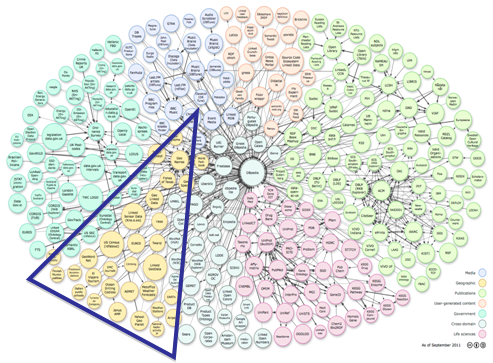
\includegraphics[scale=0.9]{img/lod-diagram-2011.png}


\section{Research Questions}
\label{sec:questions}

\section{Contributions}
\label{sec:contributions}

\section{Thesis Structure}
\label{sec:thesis-structure}
\clearpage

\part{ Modeling, Interconnecting and Generating Geodata on the Web}
%\vspace{3cm}
\chapter*{Part 1 - Modeling, Interconnecting and Generating Geodata on the Web}
\label{part:part1}
 \vspace{10mm}
\section*{Summary}
This part will talk about the various models/vocabs for representing geography/geometry. It will survey the state of the triple stores. It will describe particular problems (coordinate systems, etc.) and highlight our contributions: new vocabularies, an online converter between CRS, etc. It will describe how geography database can then be converted into RDF (Datalift processes). It will then show how those datasets can be interlinked (possibly trying different instance matching tools) and it will conclude with a thorough analysis of those alignments together with an application that could make use of those links.

%\clearpage 

%%In reality chapter 2 in the document
%% after the introduction %%%%

\chapter{Geospatial Data on the Web}
\label{ch:ch1}

\begin{itemize}
\item Traditional GIS data
\item soA on vocabularies
\item Contributions
\item conclusion
\end{itemize}

\section{Introduction}
\todo{REUSE: this section below}
The increasing number of initiatives for sharing geographic information on the web of data has significantly contribute to the interconnection of many data sets exposed as RDF based on the Linked Data principles. Many domains are represented in the web of data (media, events, academic publications, libraries, cultural heritage, life science, government data, etc.) while DBpedia is the most used dataset for interconnection. For many datasets published, geospatial information is required for rendering data on a map. In the current state of the art, different approaches and vocabularies are used to represent the ``features'' and their geometric shape although the POINT is the most common representation making use of the latitude/longitude properties defined in the W3C Geo vocabulary. Other geometries from the OpenGIS standard (POLYGON, LINESTRING, etc.) are more rarely exploited (e.g. LinkedGeoData, GeoLinkedData) while fine-grained geometry representations are often required.

In France, the National Geographic Institute (IGN) has started to publish more and more data in RDF, as illustrated by the recent experimental LOD service \url{http://data.ign.fr}. IGN maintains large databases composed of descriptions of addresses, buildings, topographic information, occupied zones, etc. A few years ago, IGN has developed a core ontology named GeOnto for describing all types of buildings located in the French territory. Integrating these databases will enable answering more complex queries than current GIS systems can handle, such as: ``\emph{show all buildings used as tribunal courts in the 7th Arrondissement of Paris}''. Another use-case is the possibility to reason over parts of a structure: ``\emph{show the points where the river Seine touches a boundary of a district in Paris that contain an activity zone}''.


\section{Geographic Information}
\todo{Use some materials from Deliverable spatial data of Datalift} \\
ADD part of the work of Nathalie thesis \\
ADD also Ruas thesis \\


 \subsection{Specificities}
 \subsection{Formats}

\section{Vocabularies for Geospatial Data}
\textcolor{red}{Add here the studies of Atemezing:TC12, with update to the current state }

The recent publication of statistics concerning the actual usage of vocabularies on the LOD cloud\footnote{\url{http://stats.lod2.eu}} provides not only an overview of best practice usage recommended by Tim Berners-Lee\footnote{\url{http://www.w3.org/DesignIssues/LinkedData.html}}, but also provides a rapid view of the vocabularies re-used in various datasets and domains. Concerning the geographic domain, the results show that W3C Geo\footnote{\url{http://www.w3.org/2003/01/geo/wgs84_pos}} is the most widely used vocabulary, followed by the \texttt{spatialrelations}\footnote{\url{http://data.ordnancesurvey.co.uk/ontology/spatialrelations}} ontology of Ordnance Survey (OS). At the same time, the analysis reveals that the property \texttt{geo:geometry} is used in $1,322,302,221$ triples, exceeded only by the properties \texttt{rdf:type} ($6,251,467,091$ triples) and \texttt{rdfs:label}\\($1,586,115,316$ triples). This shows the importance of geodata on the web. Table~\ref{tab:vocabLOD} summarizes the results for four vocabularies (WGS84, OS spatial relation, Geonames ontology and OS admin geography) where the number of datasets using these vocabularies and the actual number of triples are computed.
\begin{table*}[!htbp]
\centering{
\begin{tabular}{|l|c|r|c| }
\hline
\multicolumn{1}{|c|} {Ontologies} & \multicolumn{1}{c|}{\#Datasets} & \multicolumn{1}{c|}{\#Triples}& \multicolumn{1}{c|}{SPARQL endpoint}\\
\hline
W3C Geo  &   21 & 15 543 105 & LOD cache\\
OS spatialrelations &   10 & 9 412 167 & OS dataset\\
Geonames ontology &   5 & 8 272 905 & LOD cache\\
UK administrative-geography &   3 &  229 689 & OS dataset \\
\hline
\end{tabular}
\caption{Statistics on the usage of the four main geographic vocabularies (LOD cache should be understood as \texttt{http://lod.openlinksw.com/sparql/}). There are many more vocabularies used in the LOD cloud that contain also geographical information but that are never re-used.}
\label{tab:vocabLOD}
}
\end{table*}

\section{Current Modeling Approach}
\todo{introduce with some few words}

\subsection{Vocabularies for Features}
Modeling of features can be grouped into four categories depending on the structure of the data, the intended purpose of the data modeling, and the (re)-use of other resources.
\begin{itemize}
  \item (i): One way for structuring the features is to define high level codes (generally using a small finite set of codes) corresponding to specific
      types. Further, sub-types are attached to those codes in the classification. This approach is used in the Geonames ontology\footnote{\url{http://geonames.org/ontology/ontology_v3.0.rdf}} for codes and classes (A, H, L, P, R, S, T, U, V), with each of the letter corresponding to a precise category (e.g: A for administrative borders). Classes are then defined as \texttt{gn:featureClass a skos:ConceptScheme}, while codes are \texttt{gn:featureCode a skos:Concept}.
  \item (ii): A second approach consists in defining a complete standalone ontology that does not reuse other vocabularies. A top level class is used under which a taxonomy is formed using the \texttt{rdfs:subClassOf} property. The LinkedGeoData ontology\footnote{\url{http://linkedgeodata.org/ontology}} follows this approach, where the $1294$ classes are built around a nucleus of $16$ high-level concepts which are: \texttt{Aerialway, Aeroway, Amenity, Barrier, Boundary, Highway, Historic, Landuse, Leisure, ManMade},\\ \texttt{Natural, Place, Power, Route, Tourism, Waterway}. The same approach is used for the French GeOnto ontology (Section~\ref{sec:alignment}), which defined two high-level classes \texttt{ArtificialTopographyEntity} and \texttt{Natural\-TopographyEntity} with a total of $783$ classes.
  \item (iii): A third approach consists in defining several smaller ontologies, one for each sub-domain. An ontology network is built with a central ontology used to interconnect the different other ontologies. One obvious advantage of this approach is the modularity of the conceptualizing which should ease as much as possible the reuse of modular ontologies. Ordnance Survey (OS) follows this approach providing ontologies for administrative regions\footnote{\url{http://www.ordnancesurvey.co.uk/ontology/admingeo.owl}}, for statistics decomposition\footnote{\url{http://statistics.data.gov.uk/def/administrative-geography}} and for postal codes\footnote{\url{http://www.ordnancesurvey.co.uk/ontology/postcode.owl}}. The \texttt{owl:imports} statements are used in the core ontology. Similarly, GeoLinkedData makes use of three different ontologies covering different domains.
  \item (iv): A fourth approach consists in providing a \textit{nearly flat list} of features or points of interest. This is the approach followed by popular Web APIs such as Foursquare types of venue\footnote{\url{http://aboutfoursquare.com/foursquare-categories/}} or Google Place categories\footnote{\url{https://developers.google.com/maps/documentation/places/supported_types}}. For this last approach, we have built an associated OWL vocabulary composed of alignments with other vocabularies.
\end{itemize}

\subsection{Vocabularies for Geometry Shape}
The geometry of a point of interest is also modeled in different ways. We complete here the survey started by Salas and Harth~\cite{Salas2011}:
\begin{itemize}
  \item \textit{Point representation}: the classical way to represent a location by providing the latitude and longitude in a given coordinate reference system (the most used on the web is the WGS84 datum represented in RDF by the W3C Geo vocabulary). For example, Geonames defines the class \texttt{gn:Feature a skos:ConceptScheme} as a \texttt{SpatialThing} in the W3C Geo vocabulary.
  \item \textit{Rectangle} (``bounding box''): which represents a location with two points or four segments making a geo-referenced rectangle. In this way of modeling, the vocabulary provides more properties for each segment. The FAO Geopolitical ontology\footnote{\url{http://www.fao.org/countryprofiles/geoinfo/geopolitical/resource/}} uses this approach.
  \item \textit{List of Points}: the geometry shape is a region represented by a collection of points, each of them being described by a unique RDF node identified by a lat/lon value. The \texttt{Node} class is used to connect one point of interest with its geometry representation. The POI are modeled either as \texttt{Node} or as \texttt{Waynode} (surfaces). This approach is followed by LinkedGeoData~\cite{linkedgeodata}.
  \item \textit{Sequence of Points}: the geometry shape is represented by a group of RDF resources called a ``curve'' (similar to LineString of GML). The POI is connected to its geometry by the property \texttt{formedBy} and an attribute \texttt{order} to specify the position of each node in the sequence. This approach is the one used in GeoLinkedData~\cite{deLeon2010}.
  \item \textit{Literals}: the vocabulary uses a predicate to include the GML representation of the geometry object, which is embedded in RDF as a literal. This approach is followed by Ordance Survey~\cite{Goodwin2008}.
  \item \textit{Structured representation}: the geometry shape is represented as a typed resource. In particular, polygons and lines are represented with an RDF collection of basic W3C Geo points. This approach is used by the NeoGeo vocabulary\footnote{\url{http://geovocab.org/doc/neogeo/}}.
\end{itemize}

\subsection{GeoSPARQL Standard and specifications}
OGC has adopted the GeoSPARQL standard to support both representing and querying geospatial data on the Semantic Web. The standard document~\cite{ogc2012} contains 30 requirements. It also defines a vocabulary for representing geospatial data in RDF and provides an extension to the SPARQL query language for processing geospatial data. The proposed standard follows a modular design with five components: 
\begin{itemize}
\item (i) A \textit{core component} defining top-level RDFS/OWL classes for spatial objects; 
\item (ii) a \textit{geometry component} defining RDFS data types for serializing geometry data, RDFS/OWL classes for geometry object types, geometry-related RDF properties, and non-topological spatial query functions for geometry objects; 
\item (iii) a \textit{geometry topology component} defining topological query functions; 
\item (iv) a \textit{topological vocabulary component} defining RDF properties for asserting topological relations between spatial objects; and 
\item (iv) a \textit{query rewrite component} defining rules for transforming a simple triple pattern that tests a topological relation between two features into an equivalent query involving concrete geometries and topological query functions.
\end{itemize}

 Each of the components described above has associated requirements. Concerning the vocabulary requirements, Table~\ref{tab:reqgeosparql} summarizes the seventeen requirements presented in the GeoSPARQL draft document.
\begin{table}
\centering{
\begin{tabularx}{\textwidth}{|X|X|l|}%{l|l|l}
\hline
Geo- 	& Requi-   & Implementation Definition \\ 
Aspect	& rement   &  \\ \hline
     	 		    & Req 2 		& The Class \texttt{SpatialObject} should be defined \& accepted\\
     	 		    & Req 3 		& Defines \texttt{Feature rdfs:subClassOf SpatialObject} \\
Feature			& Req 4 			& Defines $8$ Simple Features Object Properties(OP) \\
				& Req 5 			& Defines $8$ Egenhofer OP with domain and range \\
				& Req 6			  & Defines $8$ RCC OP with domain and range \\ \hline
				& Req 7 			& Defines \texttt{Geometry rdfs:subClassOf SpatialObject} \\
Geometry		& Req 8 			& Defines OP \texttt{hasGeometry} and \texttt{defaultGeometry} \\
				& Req 9 			& Defines $6$ Data Properties: e.g: \texttt{dimension, isEmpty, etc.}  \\ \hline
				& Req 10-13			& \texttt{wktLiteral} definitions \& URI encoding  \\
Seriali- 	& Req 14			& Defines \texttt{asWKT} to retrieve WKTLiteral  \\
	zation			& Req 15-17			& GMLLiteral should be accepted  \\
				& Req 18			& Defines \texttt{asGML} to retrieve GMLLiteral \\
\hline
\end{tabularx}
\caption{Requirements and implementations for vocabulary definitions in GeoSPARQL.}
\label{tab:reqgeosparql}
}
\end{table}


\subsection{Geospatial Vocabularies and Topological Functions}
\label{sec:topofunc}
\todo{update the information in this section}

Based on the GeoSPARQL requirements, we were interested in comparing some geospatial vocabularies\footnote{\url{http://labs.mondeca.com/dataset/lov/vocabularySpace_Space.html}} to see how far they take already into account topological functions and which are the standard they followed among OpenGIS Simple Features (SF), Region Connection Calculus (RCC) and Egenhofer relations. We find that the NeoGeo (Spatial and Geometry) and OS Spatial vocabularies have integrated in their modeling partial or full aspects of topological functions as summarized in Table~\ref{tab:geosparql}.

As geodata has to be stored in triple stores with efficient geospatial indexing and querying capabilities, we also survey the current state of the art  in supporting simple or complex geometries and topological functions compatible with SPARQL 1.1. Table~\ref{tab:triplestore} shows which triple stores can support part of the GeoSPARQL standard regarding serialization and spatial functions.
\begin{table}
\begin{tabularx}{\textwidth}{|X|X|X|X|l}
\hline
\textbf{Geo-vocabulary} & \textbf{Topological Functions} & \textbf{GeoSPARQL Requirements} & \textbf{Standard Followed}\\
\hline
Ordnance Survey Spatial & \texttt{easting, northing, touches, within, contains} & Part of Req 4 & OpenGIS Simple Feature\\ \hline
Ordnance Survey Topography & \texttt{contains, isContainedIn} & Very small part of Req 4 & OpenGIS Simple Feature\\ \hline
Place Ontology & \texttt{in, overlaps, bounded\_by} & Small part of Req 4 & N/A\\
\hline
NeoGeo Spatial & All RCC8 relations & Part of Req 3; Req 6 & Region Connection Calculus (RCC)\\
\hline
NeoGeo Geometry & --- & Req 10 - 14 & N/A\\
\hline
FAO Geopolitical & \texttt{isInGroup, hasBorderWith} & -- & --\\
\hline
OntoMedia Space & \texttt{adjacent-below, adjacent-above, orbit-around, is\_boundary-of, has-boundary} & -- & --\\
\hline
\end{tabularx}
\caption{Comparison of some geo-vocabularies with respect to the GeoSPARQL requirements.}
\label{tab:geosparql}
\end{table}


\section{Georeferencing data on the Web}
\label{sec:georef}
Georeferencing data either by direct or indirect spatial reference requires some reference datasets that can be used as the spatial frame for anchoring these thematic data. Especially, it requires data on both CRSs and named places, which must be published on the Web of data.

\subsection{Identifying and describing CRSs on the Web}
In order to fulfill the need for CRS identification and description on the Web, OGC maintains a set of URIs for identifying the most commonly used CRS. While very useful, the main disadvantage of this proposal is that the URIs defined by OGC are not very intuitive for users who are not familiar with Spatial Reference System Identifiers defined by geographic information authorities like OGC or EPSG, such as ``4326'' (which actually refers to a WGS84 CRS defined by the EPSG). Moreover, many CRS commonly used locally, such as deprecated French projected CRS, are not available in that registry. In addition to OGC proposal, several registries have been proposed by the geographic information community for cataloguing existing CRSs.
The EPSG Geodetic Parameter Registry\footnote{\url{http://www.epsg-registry.org/}} allows querying the Geodetic Parameter Dataset gathered by the EPSG. CRSs can be retrieved by name, by code, by type or by coverage area, and their characteristics are displayed on a HTML form. Unfortunately, there is no direct access to these data through dereferenceable URIs.

\subsection{Direct georeferencing of data on the Web}
\label{sec:directgeo}
Modeling direct location information such as coordinates or vector data geometries in RDF still poses some challenges. \textcolor{red}{In~\cite{Atemezing:TC12}}, we have conducted a survey of the vocabularies used for representing geographical features from vocabularies of feature types to vocabularies for geometric primitives which provide ways for representing extents, shapes and boundaries of those features. 
Most of vocabularies dedicated to geometry representation reuse W3C Geo vocabulary which allows only WGS84 coordinates, such as NeoGeo\footnote{\url{http://geovocab.org/doc/neogeo/}}. With the rise of the Open Data movement, more and more publishers including governments and local authorities are releasing legacy data that are georeferenced using others CRSs. For example, IGN France releases data using different projected CRSs depending on the geographic extent of each dataset. In order to overcome this limitation on CRSs, the vocabulary designed by OGC GeoSPARQL standard  does not reuse W3C Geo vocabulary but proposes another class ``Point'' instead. Geometries of geographical data represented in RDF with the GeoSPARQL vocabulary are represented by literals encoded consistently with other OGC standards. \texttt{gsp:wktLiteral} and \texttt{gsp:gmlLiteral} are thus respectively derived from Well-Known Text and GML encoding rules. In \texttt{wktLiteral} and \texttt{gmlLiteral}, the CRS used to define the coordinates of the point is identified by a dereferenceable URI which is explicitly stated at the beginning of the literal. This way of associating coordinate reference systems with geometries has the advantage of being consistent with Linked Data principles: each CRS is identified with a dereferenceable URI. The main drawback is that such literals cannot be easily queried with SPARQL, unless using regular expression-based filters.  To overcome this limitation, we propose in the geometry vocabulary presented in \textcolor{red}{Section 3} to associate each geometry to the CRS used by its coordinates with the property \texttt{geom:crs}.

\subsection{Indirect georeferencing of data on the Web}
\label{sec:indirectgeo}
Modeling indirect location information such as administrative units or named points of interest in RDF is preferably done by identifying such geographic features with URIs and describing them by their properties, so that they can be referenced by other datasets. This is the case in one of the most reused datasets of the Web of data, namely Geonames\footnote{\url{http://sws.geonames.org/}}. However, there are yet very few reference datasets for the French territory on the Web of data.  A simple example is the current resource for \textit{Paris} in the French DBpedia\footnote{\url{http://fr.dbpedia.org/resource/Paris}}. The department's name associated to this resource is a literal named ``Paris'' and the different arrondissements composing the city are modeled as \texttt{skos:Concept} instead of \texttt{dbpedia-owl:Place}. Even Geonames data remain very limited, as French administrative units are provided as simple geometries (POINT). The ``Official Geographic Code''\footnote{\url{http://rdf.insee.fr/sparql}} published by the French Statistical Institute (INSEE) is the most up-to-date and accurate dataset on French administrative units, but unfortunately it contains no geometrical description of their boundaries. This has the consequence of not having a baseline during mapping process for application developers trying to consume specific data coming from France. Datasets describing administrative units, points of interest or postal addresses with their labels and geometries, and identifying these features with URIs could be used with benefits not only for georeferencing other datasets, but also for interlinking datasets georeferenced by direct and indirect location information.


\textcolor{red}{Describe the contributions on geometry and geography vocabularies. Reuse mainly the recent work to be presented at Terra Cognita 2014}


\section{A REST Service for Converting Geo Data}
\label{sec:rest-service}
\todo{extend this section with current results of the implementations, comparison with existing tools}

As we have seen, geodata interpretation relies on a coordinate reference system, and while the WGS84 CRS is the \textit{de-facto} standard for GPS devices, many other CRS are in used. For example LAMBERT 93, RGM 04 or RGR 92 are respectively used for georeferencing points of interests in France continental, Mayotte or La Reunion. We have developed a REST service that is capable of transforming one dataset using a particular CRS into another one. The algorithms implemented are the ones described at \url{http://geodesie.ign.fr/index.php?page=algorithmes} and available within the standalone Circ\'e software\footnote{\url{http://fr.wikipedia.org/wiki/Circe_(logiciel)}}. Some existing tools like Circ\'e or the the world coordinate converter\footnote{\url{http://twcc.free.fr.are}} are good as a standalone tool for end user, but not so great for developers,  as they can only use them to test their result. There is no possible way to use their fully function algorithm unless develop it again.  At the moment, the following features are implemented:
\begin{itemize}
\item from/to WGS 84 to/from WGS 84 UTM ;
\item from/to WGS 84  to/from Lambert 93 and 
\item from/to WGS 84 UTM to/from Lambert 93
\end{itemize}   

The API can also convert a file with space separated values. The API supports JSON as one of the output format. The code of the REST service is available at \url{https://github.com/vienlam/Geo}.

\subsection{Algorithms Evaluation}

\subsection{API Access and Parameters}

\subsection{User Interface}

\begin{figure}[!htbp]
\centering{
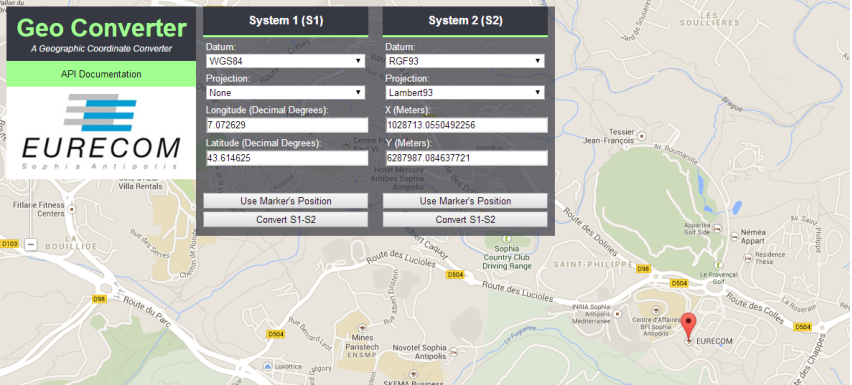
\includegraphics[scale=0.9]{img/UIconverter.pdf}
\caption{The UI of the converter}
\label{fig:uiconverter}
 }
\end{figure}


\section{Best Practices for Modeling Geospatial vocabularies}
\label{sec:bpgeo}

In~\cite{Atemezing:TC12}, we already surveyed numerous vocabularies for representing geographical features and their geometries, either using a literal (e.g. wktLiteral) or a structured representation \`a la NeoGeo. We concluded the survey with some recommendations for geometry descriptions:
\begin{itemize}
 \item the distinction of geometry versus feature and a property linking both classes (e.g. for attaching provenance information on how some points of a geometry have been collected),
 \item the ability to represent structured geometries (e.g. for performing simple spatial queries on the data, even when they are stored in a triple store that do not implement the GeoSPARQL standard),
 \item the integration of any coordinate reference system  (e.g. for allowing projected coordinates for cartographic purposes).
\end{itemize}
In addition to these recommendations, we also think that the domain of the property used to link a feature to its geometry should be left empty in order to accept links between any type of resource and a geometry. This would be useful for example, to associate a person to the coordinates of their birthplace.

\subsection{Some Recommendations}
The alignment of GeOnto provided in the \textcolor{red}{previous section} enables interoperability of symbolic descriptions. The need for a better choice of geometric structure, typically the choice between literal versus structured representations depends on three criteria: (i) the coverage of all the complex geometries as they appear in the data; (ii) a rapid mechanism for connecting ``features'' to their respective ``geometry''; (iii) the possibility to serialize geodata into traditional formats used in GIS applications (GML, KML, etc.) and (iv) the choice of triple stores supporting as many as possible functions to perform quantitative reasoning on geodata. It is clear that a trade-off should be taken depending on the technological infrastructure (e.g: data storage capacity, further reasoning on specific points on a complex geometry).

\begin{itemize}
\item\textbf{Complex Geometry Coverage:} We have seen that on the Web of Data, there are few modeling of geodata with their correct shape represented as a LINE or POLYGON. However, some content providers (e.g. IGN) need to publish all types of geodata including complex geometries representing roads, rivers, administrative regions, etc. Two representations are suitable: \textit{OS Spatial} and \textit{NeoGeo} ontologies (Table~\ref{tab:reqgeosparql}). Direct representation of the GeoSPARQL vocabulary is also suitable.
\item \textbf{Features connected to Geometry:} In modeling geodata, we advocate a clear separation between the features and their geometry. This is consistent with the consensus obtained from the different GeoVocamps\footnote{\url{http://www.vocamp.org}} and the outcome of this approach is expressed in the modeling design of NeoGeo. The top level classes \texttt{spatial:Feature} and \texttt{geom:Geometry}are connected with the property \texttt{geom:geometry}.

\item \textbf{Literal versus structured Geometry:} Decomposing a LINE or a POLYGON into multiple results in an ``explosion'' in the size of the dataset and the creation of numerous blank nodes. However, sharing points between descriptions is a use case with such a need. IGN has such use-cases and the natural solution at this stage is to consider reusing the NeoGeo ontology . The choice of the triple store (e.g.,Virtuoso vs Open Sahara) is not really an issue, as the IndexingSail\footnote{\url{https://dev.opensahara.com/projects/useekm/wiki/IndexingSail}} service could also be wrapped on-top of Virtuoso to support full OpenGIS Simple Features functions\footnote{\url{http://www.opengeospatial.org/standards/sfs}}.
\end{itemize}


\section{Vocabularies for Geometries and Feature Types} \label{sec:topovocab}

Direct georeferencing of data implies representing coordinates or geometries and associating them to a CRS.  This requires vocabularies for geometries and CRSs. Besides, indirect georeferencing of data implies associating them to other data on named places. Preferably, these data on named places should be also georeferenced by coordinates in order to serve as basis for data linking between indirectly and directly georeferenced datasets. In this section, we present the vocabularies that we have defined and reused for geographic data publishing.
This requires reference geographic data on named places and therefore vocabularies for describing feature types and their properties. 

\subsubsection{A vocabulary for geometries} \label{sec:geomvocab}


\todo{On the current usage of georeferencing resources on the Web of data, it is assumed that the coordinates should be in WGS84, and hence the definition of the point. However, publishers might have data in different CRSs according to the location. Thus, our proposal is to define a more generic class for a POINT  with the benefit of choosing the CRS of the underlying data, as depicted in the Listing 1.1.}

\lstset{basicstyle=\scriptsize, backgroundcolor=\color{white}, frame=single, caption= {Definition in Turtle of the axiom defining a POINT. }, label=point, captionpos=b}
\begin{lstlisting}
geom:Point a owl:Class;
  rdfs:label "Point"@en, "Point"@fr;
  rdfs:subClassOf geom:Geometry;
  owl:equivalentClass
    [a owl:Class ;
	  owl:intersectionOf
		([a owl:Restriction;
		   owl:onDataRange xsd:double;
		   owl:onProperty geom:coordY;
	       owl:qualifiedCardinality "1"^^xsd:nonNegativeInteger]
         [a owl:Restriction;
		   owl:onDataRange xsd:double;
		   owl:onProperty geom:coordX;
		   owl:qualifiedCardinality "1"^^xsd:nonNegativeInteger])
     ] ;
     rdfs:subClassOf sf:Point.
\end{lstlisting}

\subsubsection{Extending GeoSPARQL vocabulary}
In order to fulfill these recommendations, we have developed a new vocabulary that re-uses and extends the existing vocabularies for representing geometries, namely:
\begin{itemize}
 \item \url{http://www.opengis.net/ont/geosparql#} (prefix \texttt{gsp}). This vocabulary provides the basic concepts to represent geographical data such as SpatialObject, Feature or \texttt{Geometry}. A Feature is linked to a Geometry via the relation \texttt{gsp:hasGeometry}. The geometries are typed strings (\texttt{gsp:gmlLiteral} or \texttt{gsp:wktLiteral} corresponding respectively to the properties \texttt{gsp:asGML} and \texttt{gsp:asWKT}). The vocabulary contains also spatial functions.
 \item \url{http://www.opengis.net/ont/sf#} (prefix \texttt{sf}): This vocabulary is based on the OGC standard Simple Features Access \cite{iso2004}. The class \texttt{sf:Geometry} is a subclass of \texttt{gsp:Geometry}. 
\end{itemize}
 
Reusing and extending GeoSPARQL Simple Features vocabulary with structured geometries  \`a la NeoGeo enables us to represent geometries both with GeoSPARQL compliant literals and with structured geometries that can be handled easily with SPARQL. The extension for structured geometries consists in defining a subclass for each class from the \texttt{sf} vocabulary, and defining properties to associate its instances with a CRS and coordinates or other suitable geometric primitives. For example, the class \texttt{geom:Point} is a subclass of \texttt{sf:Point}. An instance of \texttt{geom:Point} is associated with exactly one instance of \texttt{ignf:CRS} via the property \texttt{geom:crs}, and it
has exactly one coordinate X and exactly one coordinate Y. It can also have a Z coordinate. The coordinates are \texttt{xsd:double} and correspond to the properties \texttt{geom:coordX:}, \texttt{geom:coordY:} and \texttt{geom:coordZ:} respectively. Other complex geometries are also defined, such as Linestrings, LinearRings, Polygons or MultiPolygons. Their definitions are based on the class \texttt{geom:Point}. As an example, an instance of \texttt{geom:Linestring} is defined as an instance of \texttt{geom:PointsList} which is an ordered \texttt{rdf:List} of instances of \texttt{geom:Point} designated by the property \texttt{geom:points}.


We have also defined a property \texttt{geom:geometry} with an empty domain. Thus, our proposal defines a more generic class for a \textsf{POINT} with the benefit of choosing the CRS of the underlying data. Figure \ref{fig:geomcrs} gives an overview of the relationships between the high level concepts with geometries, CRS and topographic features.

\begin{figure}[!htbp]
\vspace{-13pt}
  \begin{center}
  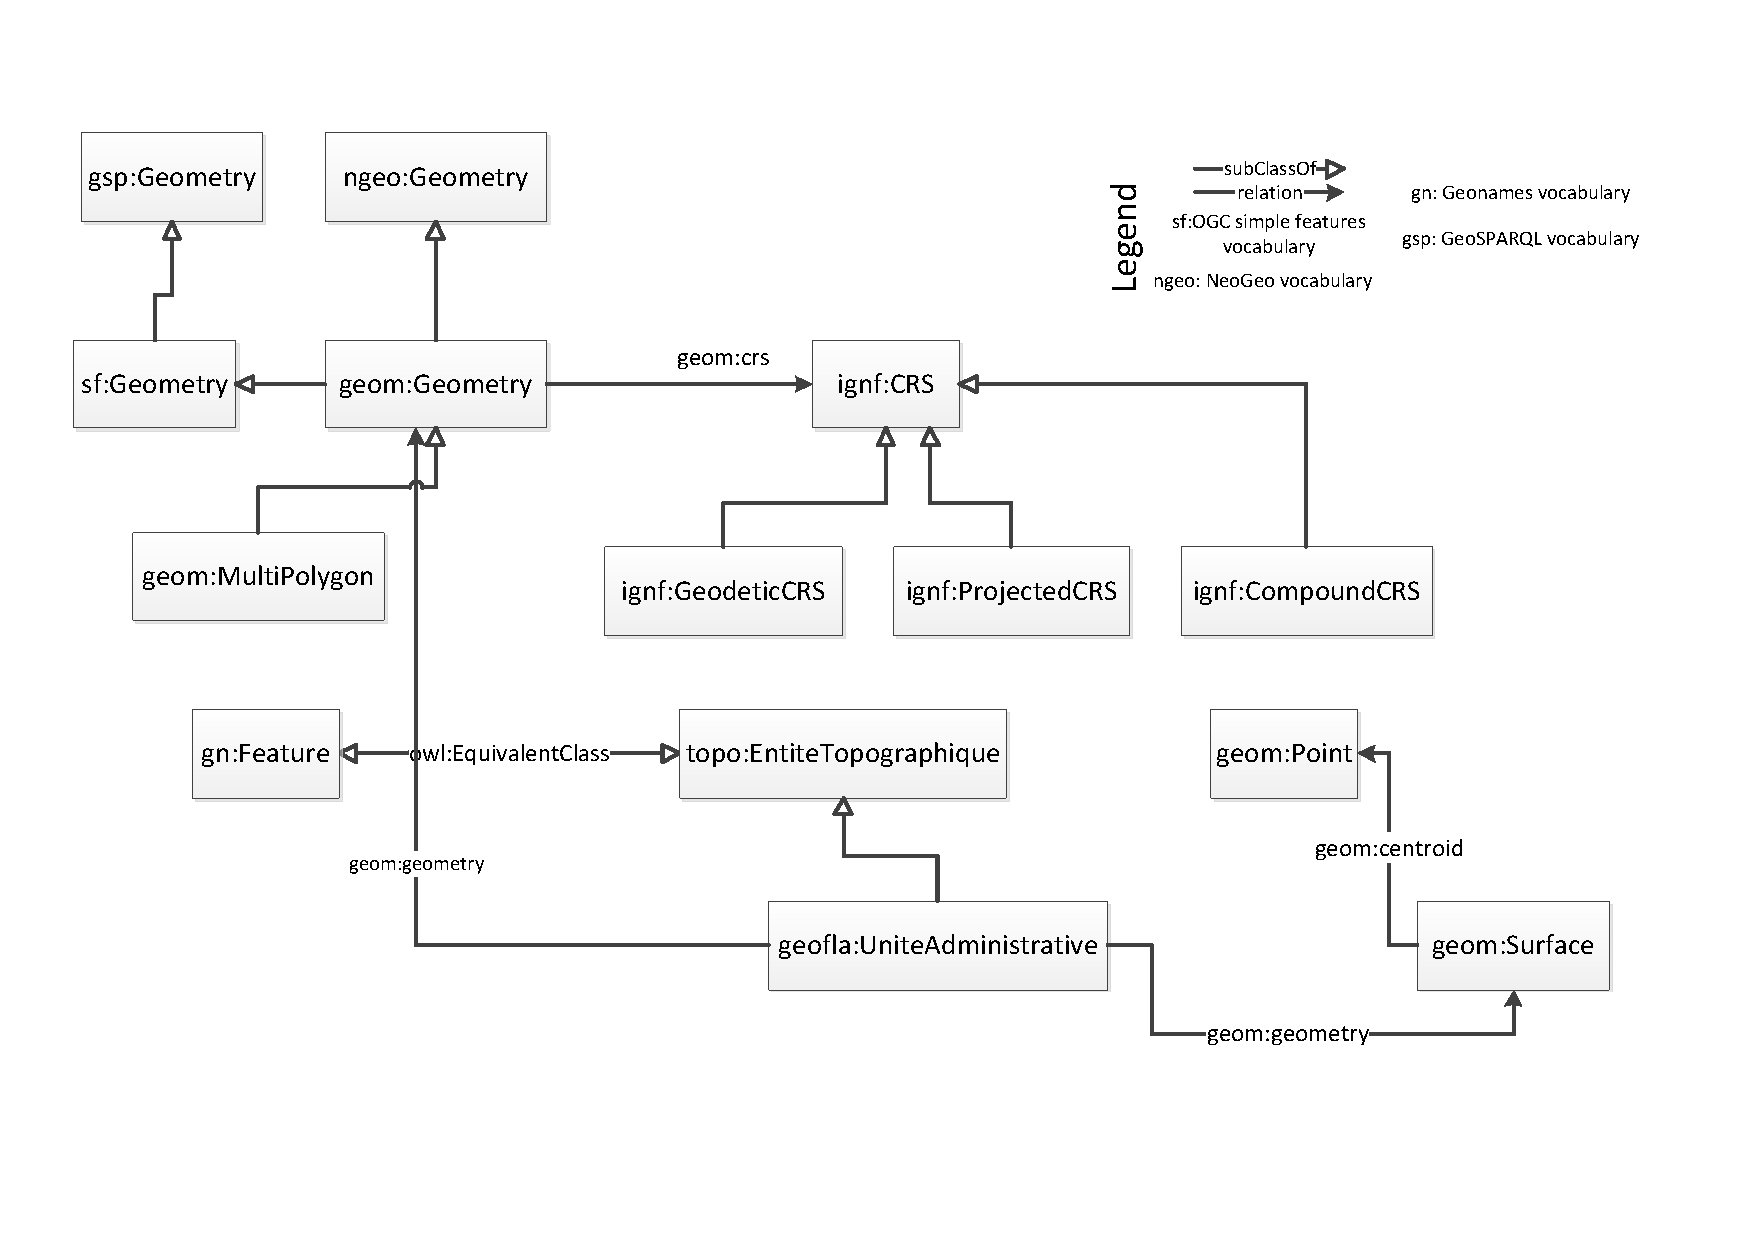
\includegraphics[width=0.8\textwidth]{img/vocabs-ign.pdf}
  \vspace{-15pt}
  \caption{High level classes of ignf, geom and topo vocabularies; relationships between them and mappings with external vocabularies.}
  \vspace{-10pt}
  \label{fig:geomcrs}
  \end{center}
\end{figure}

\textcolor{red}{
\subsection{Publishing structured geometries from geographic data}
The vocabulary for geometry reused by a geodata converter that takes traditional GIS data as input and outputs RDF data with geometries defined both with a \texttt{gsp:wktLiteral} and with a structured representation compliant with our vocabulary. Geometries are automatically associated with the chosen CRS. This converter is implemented as a plugin of the Datalift platform \todo{reference section} and can be reused easily for geographic data publishing purpose.
}

\subsection{CRS requirements for the  French territory} \label{sec:reqs}

As explained in Section \ref{sec:context}, making explicit the CRS used in a given dataset is a very important issue when dealing with direct location data. This is especially important in the field of geographical information where different CRSs are commonly used due to technical or legal requirements. For INSPIRE Directive, CRS are considered as reference data used for linking thematic data \cite{inspire2009}, and must be described according to ISO 19111 standard. To be consistent with Linked Data principles, CRS should be identified by URIs, like in OGC proposal. Moreover, as Linked Data users are not always familiar with CRS identifiers commonly used within the geographic information community, URI used to identify CRS should use more intuitive names. Finally, consistently with our goal of contributing to a better georeferencing of data on the French territory, we need an access to the descriptions of all French CRSs, including some deprecated but still used CRSs like ``Lambert 1''.



\begin{table}[!htp]
\centering{
\begin{tabular}{lr}
\specialrule{1pt}{1pt}{1pt}
 \textbf{Prefix}	& 	\textbf{URI}	  \\ \specialrule{1pt}{1pt}{1pt}
geofla 	   & \url{http://data.ign.fr/def/geofla#}  \\
geom &  \url{http://data.ign.fr/def/geometrie#} \\
ignf &  \url{http://data.ign.fr/def/ignf#} \\
rgeofla &  \url{http://data.ign.fr/id/geofla/} \\
topo &  \url{http://data.ign.fr/def/topo#} \\
rtopo &  \url{http://data.ign.fr/id/topo/} 

		\\ \specialrule{1pt}{1pt}{1pt}
\end{tabular}
\caption{ URI schemes and conventions used for vocabularies and resources.}
\label{tab:uris}
}
\end{table}

The Information and Service System for European Coordinate Reference Systems\footnote{\url{http://www.crs-geo.eu}}  provides an access to ISO 19111 standard-based descriptions of the main European CRSs but has the same limitation as the EPSG registry: access to the descriptions is not allowed by URI, but only through a cartographic interface.
\url{SpatialReference.org} initiative aims at allowing users to use URI-based references to spatial reference systems, including some CRSs defined and maintained by IGN France.  Besides, the proposed URL policy is not very intuitive. As an example, this URL identifies the projected system defined by IGN France, Lambert 93: \url{http://spatialreference.org/ref/sr-org/7527/}. Moreover, the definitions of some deprecated CRSs such as Lambert zone projected CRSs (which are still used in some datasets) seem to be referenced only for the authority EPSG and not for IGNF, which also maintains a registry of CRSs. ISO 19111 standard-based definitions of all CRSs defined and maintained by IGN France are  published in an XML file\footnote{\url{ http://librairies.ign.fr/geoportail/resources/IGNF.xml}}.
References to equivalent definitions provided by the EPSG registry are explicitly stated with EPSG SRID. CRSs are identified by URIs using short names instead of numeric codes. For example, \url{http://registre.ign.fr/ign/IGNF/crs/NTFLAMB2E}  is the URI designed for the ``Lambert 2 \'{e}tendu'' projected system. Indeed ``NTFLAMB2E'' is used to identify the projected system ``Lambert 2 \'{e}tendu'' which is based on NTF (New French Triangulation) geodetic reference system. Unfortunately, this registry is still in evolution and its URIs are not dereferenceable yet.

\begin{figure}[!htbp]
 \begin{center}
  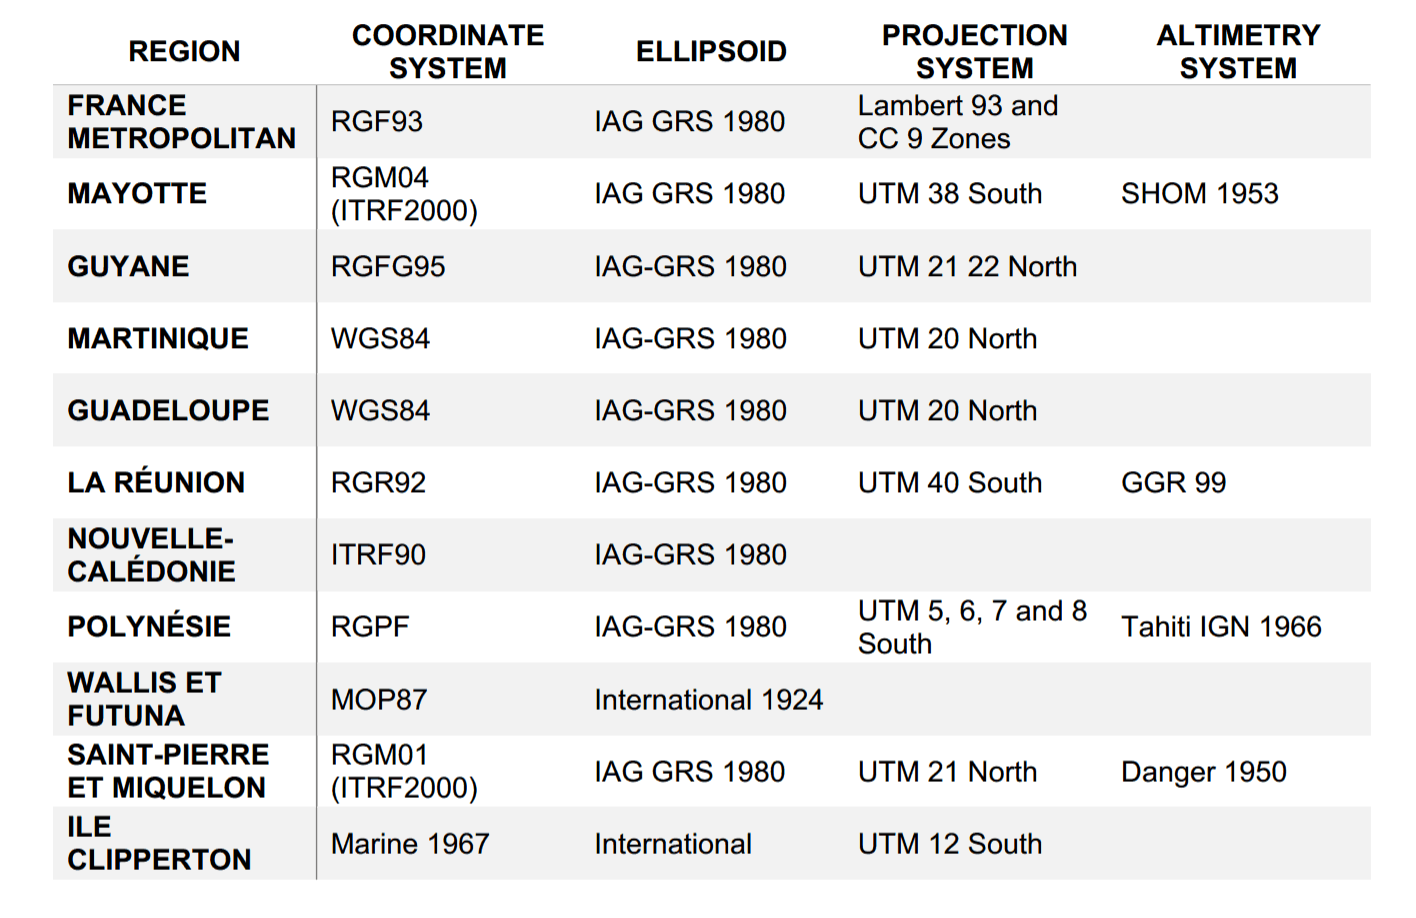
\includegraphics[width=120mm]{img/crs-france.png}
  \caption{Coordinate Reference Systems used in France. Source: \texttt{http://geodesie.ign.fr/}}
  \label{fig:crsinfr}
 \end{center}
\end{figure}
 
%\paragraph{Publishing a dataset on French CRSs}
As no existing registry fulfilled all our requirements, we have developed a vocabulary\footnote{\url{http://data.ign.fr/def/ignf}}, inspired from the ISO 19111 schema for CRSs description. Then we have converted IGNF CRSs registry into RDF, and published this dataset on the Web with the Datalift platform\footnote{A service to lookup CRS in RDF can be found at \url{http://www.eurecom.fr/~atemezin/ignf-lookup/}}. Therefore, the description of the ``NTF Lambert 2 \'{e}tendu'' projected CRS can be retrieved at this URL \url{http://data.ign.fr/id/ignf/crs/NTFLAMB2E}.

\section{Vocabularies for Geographic Feature Types}
\label{sec:vocgeofeature}

Indirect georeferencing of resources on the Web requires reference geographic data on named places and therefore vocabularies for describing feature types and their properties. Therefore, we have chosen to publish a reference dataset on administrative units called GEOFLA\circledR, which is already available in GIS format under an Open Data license. We have also made tests of data conversion and interlinking with another largest dataset on French names places. We have produced and published two vocabularies to describe these datasets, to make sure that all concepts and properties needed would be available.
In the GEOFLA\circledR ~vocabulary, 5 classes have been defined: commune, canton, arrondissement, department and region. In the BD TOPO\circledR ~vocabulary\footnote{\url{http://data.ign.fr/def/topo}} $35$ main classes have been defined. They represent the main types of geographic features represented in the BD TOPO\circledR ~database. In both vocabularies, properties have been defined based on the attributes of their related classes in the databases. The geographic feature types defined as values of attributes ``nature'' are modeled as instances of \texttt{skos:Concept}. SKOS is intensively used to easily group concepts into different schemes (using \texttt{skos:hasTopConcept}) and provide semantic relationships (e.g: \texttt{skos:broader}, \texttt{skos:narrowMatch}) among them. We also provide alignments with Geonames vocabulary, where \texttt{topo:Place} is subclass of \texttt{gn:S} and \texttt{owl:sameAs} linked concepts.\footnote{\url{https://github.com/gatemezing/ign-iswc2014/blob/master/vocabularies/mappingsGeonames.ttl}} 

All the classes are defined as subclasses of  \texttt{topo:EntiteTopographique} which defines the representation of a real world entity associated to a location relative to the Earth, consistently with ISO TC 211 and OGC standards. 
The GEOFLA\circledR 's application schema is composed of classes representing different types of french administrative units, namely communes, cantons, arrondissements and departments. In \texttt{geofla} vocabulary, we add a class region  from the instances of the class department via two attributes  that precise to what region each instance of department belongs.  Their properties are defined based on the attributes of their related classes in GEOFLA\circledR ~database.

\textcolor{red}{Regarding use cases consuming  real-world databases developed using the vocabularies aforementioned, two different applications have been developed. namely \textit{PerfectSchool}\footnote{\url{semantics.eurecom.fr/datalift/PerfectSchool/}}  and \textit{Equipment}\footnote{\url{http://semantics.eurecom.fr/datalift/Equipment/}}. The former is a mobile application intended to provide useful information on schools in France, while the latter is a facet view by categories of facilities in France, specifically in the city of Toulouse. }
A Commune has an attribute called \textit{``nature''} whose enumerated values precise whether the commune is the capital of a bigger administrative unit, modeled in the vocabulary by the ObjectProperty \texttt{geofla:statut} with range \texttt{skos:Concept} defined in this specific \texttt{skos:ConceptScheme} \url{http://{BASE}/codes/geofla/typedecommune/liste} pointing to the different types of French administrative unit's capital. 






\clearpage


\chapter{Publishing and Querying Geodata }
\label{ch:ch2}

\begin{itemize}
\item steps for publishing geodata--existing tools
\item soA on triple stores 
\item interconnections and 5-stars datasets
\item Datalift for geo data
\item contrib for french publications
\end{itemize}

\section{Existing Tools for Converting Geospatial Data}
\label{sec:toolgeo}



\section{Geodata Providers and Access}
So far, the Web of data has taken advantage of geocoding technologies for publishing large amounts of data. For example, Geonames provides more than 10 millions records (e.g. $5,240,032$ resources of the form \url{http://sws.geonames.org/10000/}) while LinkedGeoData has more than $60,356,364$ triples. All the above mentioned data are diverse in their structure, the access point (SPARQL endpoint, web service or API), the entities they represent and the vocabularies used for describing them. Table~\ref{tab:srce-data} summarizes for different providers the number of geodata available (resources, triples) and how the data can be accessed.
\begin{table}[!htbp]
\centering{
\begin{tabular}{|ll|r|r|}
\hline
\multicolumn{2}{|c}{\textbf{Provider}} & \multicolumn{1}{|c}{\textbf{\#Geodata}} & \multicolumn{1}{|c|}{\textbf{Data access}}\\
\hline
\multicolumn{2}{|l|}{DBpedia} & 727 232 triples & SPARQL endpoint\\
\multicolumn{2}{|l|}{Geonames} & 5 240 032 (feature). &  API \\
\multicolumn{2}{|l|}{LinkedGeoData} & 60 356 364 triples & SPARQL endpoint, Snorql\\
\multicolumn{2}{|l|}{Foursquare} & n/a & API\\
\multicolumn{2}{|l|}{Freebase} & 8,5MB  & RDF Freebase Service\\
\multicolumn{2}{|l|}{Ordnance Survey(Cities)} & 6 295 triples  & Talis API \\
\multicolumn{2}{|l|}{GeoLinkedData.es} & 101 018 triples  & SPARQL endpoint \\
\multicolumn{2}{|l|}{Google Places} & n/a  & Google API \\
\multicolumn{2}{|l|}{GADM project data} & 682 605 triples & Web Service \\
\multicolumn{2}{|l|}{NUTS project data} & 316 238 triples & Web Service \\
\multicolumn{2}{|l|}{IGN experimental} & 629 716 triples & SPARQL endpoint \\
\hline
\end{tabular}
\caption{Geodata by provider and their different access type}
\label{tab:srce-data}
}
\end{table}


\section{Scenario: 7$^{th}$ Arrondissement of Paris}                      \label{sec:scenario}
\todo{Update the scenario with the current version of DBpedia 2014, DBpedia-FR}

The 7$^{th}$ arrondissement of Paris is one of the 20 arrondissements (administrative districts) of the capital city of France. It includes some of Paris's major tourist attractions such as the Eiffel Tower, some world famous museums (e.g: \textit{mus\'{e}e d'Orsay}) and contains a number of French national institutions, including numerous government ministries\footnote{\url{http://en.wikipedia.org/wiki/7th_arrondissement_of_Paris}}. We use it throughout this paper to highlight the diversity of representations one can use for this geographical entity. We assume that this district should be modeled as a POLYGON composed of a number of POINTs needed to ``interpolate'' its effective boundaries. We assume the use of the WGS84\footnote{\url{http://en.wikipedia.org/wiki/World_Geodetic_System}} geodetic system.

\subsection{DBpedia Modeling}
We provide below an excerpt of the DBpedia description for this resource.
{\scriptsize
\begin{verbatim}
  dbpedia:7th_arrondissement_of_Paris a gml:_Feature ;
    a <http://dbpedia.org/class/yago/1900SummerOlympicVenuEs>
    rdfs:label "7. arrondissementti (Pariisi)"@fi; (14 different languages)
    dbpprop:commune "Paris" ;
    dbpprop:departement  dbpedia:Paris ;
    dbpprop:region dbpedia:Ile-de-France_(region) ;
    grs:point "48.85916666666667 2.312777777777778" ;
    geo:geometry "POINT(2.31278 48.8592)" ;
    geo:lat "48.859165"^^xsd:float;
    geo:long "2.312778"^^xsd:float.
\end{verbatim}
}
First, we observe that the type \texttt{gml:\_Feature} and the property \texttt{grs:point} are not resolvable since there are no OWL ontologies that provide a description of them. Second, the property \texttt{geo:geometry} used by DBpedia is not defined in the WGS84 vocabulary. For the geometry, the 7th arrondissement is a simple POINT defined by a latitude and a longitude.

\subsection{Geonames Modeling}
In Geonames, the 7th arrondissement is considered as a 3$^{rd}$ order administrative division, represented by a POINT for the geometry model. The RDF description of this resource gives other information such as the alternate name in French, the country code and the number of inhabitants.
{\scriptsize
\begin{verbatim}
  gnr:6618613 a gn:Feature ;
    gn:name "Paris 07";
    gn:alternateName "7ème arrondissement";
    gn:featureClass gn:A [
      a skos:ConceptScheme ;
      rdfs:comment "country, state, region ..."@en .
    ] ;
    gn:featureCode gn:A.ADM4 [
      a skos:Concept ;
      rdfs:comment "a subdivision of a third-order administrative division"@en .
    ];
    gn:countryCode "FR";
    gn:population "57410";
    geo:lat "48.8565";
    geo:long "2.321".
\end{verbatim}
}

\subsection{LinkedGeoData Modeling}
In LinkedGeoData, the district is a \texttt{lgdo:Suburb rdfs:subClassOf ldgo:Place}. Its geometry is still modeled as a POINT and not as a complex geometry of type POLYGON as we could have expected for this type of spatial object.
{\scriptsize
\begin{verbatim}
  lgd:node248177663 a lgdo:Suburb ;
    rdfs:label "7th Arrondissement"@en , "7e Arrondissement" ;
    lgdo:contributor lgd:user13442 ;
    lgdo:ref%3AINSEE 75107 ;
    lgdp:alt_name "VIIe Arrondissement" ;
    georss:point "48.8570281 2.3201953" ;
    geo:lat 48.8570281 ;
    geo:long 2.3201953 .
\end{verbatim}
}

\subsection{Discussion}
These samples from DBpedia, Geonames and LinkedGeoData give an overview of the different views of the same reality, in this case the district of the 7$^{th}$ Arrondissement in Paris. Regarding the ``symbolic representation'', two datasets opted for ``Feature'' (DBpedia and Geonames) while LGD classifies it as a ``Suburb'' or ``Place''. They all represent the shape of the district as a POINT which is not very efficient if we consider a query such as \emph{show all monuments located within the 7th arrondissement of international importance}. To address this type of query and more complicated ones, there is a need for more advanced modeling as we describe in the next section.

\section{Benchmarking Triple Stores}
\label{sec:benchmarking}

\begin{itemize}
\item \textbf{Serialization and Triple stores:} We also advocate the use of properties that can provide compatibility with other formats (GML, KML, etc.). This choice can be triple store independent, as there could be ways to use content-negotiation to reach the same result. In Table \ref{tab:triplestore}, \texttt{Open Sahara}\footnote{\url{http://www.opensahara.com}}, \texttt{Parliament }\footnote{\url{http://geosparql.bbn.com}},  \texttt{Virtuoso}\footnote{\url{http://www.openlinksw.com}} are WKT/GML-compliant with respectively $23$ and $13$ functions dealing with geodata.
\item The choice of the triple store (e.g.,Virtuoso\footnote{Here we used Virtuoso Open Edition, V6.xx} vs Open Sahara) is not really an issue, as the IndexingSail\footnote{\url{https://dev.opensahara.com/projects/useekm/wiki/IndexingSail}} service could also be wrapped on-top of Virtuoso to support full OpenGIS Simple Features functions\footnote{\url{http://www.opengeospatial.org/standards/sfs}}.
\end{itemize}

\todo{update the table with recent data}
\begin{table}[!htbp]
 \begin{tabularx}{\textwidth}{|X|X|X|X|X|l|}
 \hline
 \textbf{Triple store} & WKT-compliance & GML-compliance & Geometry supported  & Geospatial Functions & GeoVocab \\ \hline
 Virtuoso & Yes & Yes & Point & 13 functions & W3C Geo + Typed Literal  \\ \hline
 Allegro-Graph & \-- & -- & Point & 3 functions & ``strip'' mapping data \\ \hline
 OWLIM-SE & -- & -- & Point & 4 functions & W3C Geo\\ \hline
 Open Sahara & \ Yes & Yes & Point, Line, Polygons & 23 functions  & Typed Literal \\ \hline
 Parliament & \ Yes & Yes & Point, Line, Polygons & 23 functions  &  GeoSPARQL vocabulary\\ \hline
 \end{tabularx}
\caption{Triple stores survey with respect to geometry types supported and geospatial functions implemented.}
\label{tab:triplestore}
\end{table}

\section{Publishing Addresses of OSM-France in RDF}
\label{sec:bano2rdf}

Explain briefly the requirements and work on publishing bano2RDF: vocabularies, 4 stars..
\todo{discuss here if it could be wise to use Linked Data Fragments..maybe as future work?} .



\section{Status of French Datasets in RDF}
\label{sec:frenchCloud}

\begin{figure}[h!t]
%\vspace{-2.5cm}
  \centering{
    %\leavevmode
      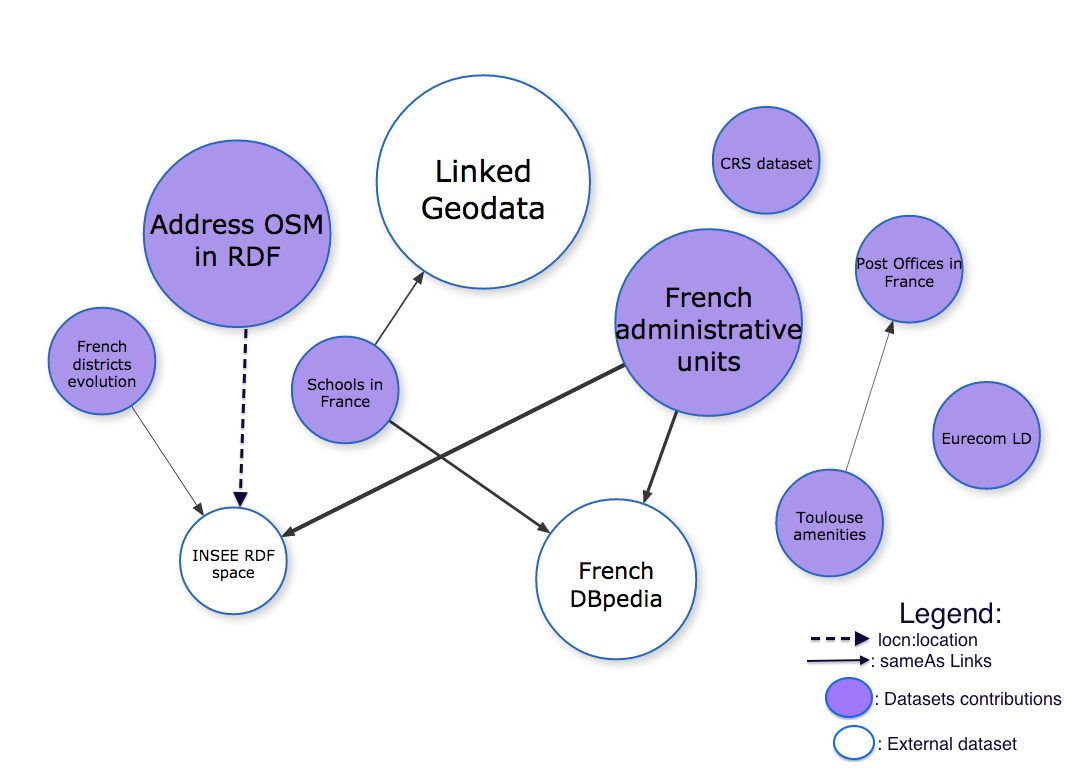
\includegraphics[width=\linewidth]{img/frenchCloud.png}
  
    \caption{French LOD Cloud based on the different datasets published in 4-5 stars. }
    \label{visuGraphModel}
  }
\end{figure}
\clearpage

%\chapter{Visualizing RDF data on the Web }
\label{ch:ch3}

\begin{itemize}
\item survey tools to visualize data
\item applications/visu for LD
\item Describing visualizations 
\item A vocab for visualizations
\end{itemize}
%\clearpage

%\chapter*{Part 2 - Generating Visualizations for Linked Data}
\label{part:part2}
 \vspace{10mm}
\section*{Summary}
This part cover three main problematics regarding how to present RDF to end-users. There is a consensus that RDF is not what is shown to the users.  First, we make a state of the art review of existing tools and solutions for visual representation and exploration of RDF (Visualbox, LODSpeaKr, Map4RDF, Linked Data Visualization Model, other works from the SWUI community, from Roberto Garcia, etc.) The, we present our contribution: the wizard for visualizations including the vocabulary for describing visualizations , the prototype itself, etc. Third, we present a  mechanism of extracting and reusing application contests in open data events, and finally we provide some insights on revealing the important properties of Entities for visualization. 
%\clearpage
\part{Generating Visualizations for Linked Data}

\chapter{Analyzing and Describing Visualization Tools and Applications}
\label{ch:ch4}

\begin{flushright}
\textit{``I think we have consensus, RDF is something \\
you don't show your end users.''\footnote{\url{https://twitter.com/philarcher1/status/507856407127814145}}}  \\
Phil Archer (W3C Data Activity Lead)
\end{flushright}


\section*{Introduction}
\label{sec:intro-ch4}

According to \cite{marti2009} the main goal of information visualization is to translate abstract information into a visual form that provides new insight about that information, in a clear and precise form. In the field of information visualization, data classification, either quantitative or categorical, is useful for visualization, and can be used to make the difference between tools. For example, hierarchical faceted metadata can be used to build a set of category hierarchies where each dimension is relevant to the collection for navigation. The resulting interface is known as faceted navigation, or guided navigation \cite{hearst02}. However, visualizing structured data in RDF by taking advantage of the underlying semantics is challenging both for the publishers and for the users. On the one hand, publishers need to build nice visualizations on top of their 4-5 star datasets (section \ref{sec:descApps}). On the other hand, lay users shouldn't need to understand the complexity of the Semantic Web stack in order to quickly get insights from the data. Thus, adapting visual tools for exploring RDF datasets can bridge the gap between the complexity of Semantic Web and simplicity offered by the field of information exploration. In this chapter, we survey tools for visualizing both structured data (section \ref{sec:strucdataviz}) and RDF data section \ref{sec:vizrdf}). We then provide a classification of the tools for creating applications in the context of LOD (section \ref{sec:discussion}), along with the way applications are described on the Web. Section \ref{sec:apps} describes Linked Data applications, followed by the relevant information to describe applications built on top of government open datasets (section \ref{sec:reusable}). The chapter ends with a brief summary.

%\textcolor{red}{In this chapter, we do X , Y and Z }

\section{Survey on Visualization Tools }
\label{sec:visu-soa}

In this section, we describe also visualization tools that natively do not take as input RDF data for two reasons:
\begin{itemize}
\item those tools are relatively ``popular'' for analyzing data exposed by the government and agencies  (most of them in XLS, CSV) as they quickly make it easy to the users  to build chart  maps and compare with other datasets. One widely application is in the data journalism  where facts are analyzed by those tools without waiting for the semantic publication of the data
\item Also these tools have many options for visualizing data and are not totally compatible with RDF resources for visualizing graphs.

\end{itemize}


\subsection{Tools for visualizing Structured Data}
\label{sec:strucdataviz}

In this section, we review tools that are used to visualize structured data and RDF data. The former categories can be extended to support RDF, while the latter tools are trying to cover visualization charts/graphs as much as possible. The authors in \cite{odm14} propose an overview of all JavaScript visualization libraries and frameworks that are open source, supporting at least bar charts, line charts and pie charts. However, the focus is rather for tools to create dashboard in open data in general, and two of the tools their report are also included in this section, such as D3.js and Google Charts.

\subsubsection{Choosel}
\label{sec:choosel}

\texttt{Choosel} \cite{lars2010} is built on top of GWT  and the Google App Engine  (the backend can be modified to run on any servlet container). The client-side framework facilitates interaction with visualization components, which can be wrappers around third party components and toolkits such as the Simile Timeline, Protovis and FlexViz. Choosel can integrate components developed using different technologies such as Flash and JavaScript. It is possible to implement visualization components that are compatible with the Choosel visualization component API. These visualization components can then be used to take advantage of Choosel features such as management of view synchronization, management of selections, and support for hovering and details on demand.

\subsubsection{Many Eyes}
\label{sec:manyEyes}
\texttt{Many Eyes} \cite{ibm2010} is a website that can be used to visualize data such as numbers, text and geographic information. It provides a range of visualizations including unusual ones such as ``treemaps''  and ``phrase trees''. All the charts made in Many Eyes are interactive, so it is possible to change what data is shown and how it is displayed. Many Eyes is also an online community where users can create groups (such as ``Ebola Crisis'' or ``Kobane War'') to organize, share and discuss data visualizations. Users can also comment on visualizations made by others, which is a good way to improve their work. The authors claim that with Many Eyes, the users ``\textit{can build quick and easily visualizations from their own data, with the possibility to share them}''. Data input formats are XLS, Plain text and HTML. The output formats are PNG or embeddable. However, using Many Eyes makes  your data and the visualizations created with it public. The license of Many Eyes is proprietary of IBM.

\subsubsection{D3.js}
\label{sec:d3js}

\texttt{D3.js} \cite{d3js} is a JavaScript library for manipulating documents based on data. D3 uses HTML, SVG and CSS. D3 combines powerful visualization components, plugins\footnote{\url{https://github.com/d3/d3-plugins}}  and a data-driven approach to Document Object Model (DOM) manipulation. D3 solves the problem of efficient manipulation of documents based on data. It avoids proprietary representation and affords flexibility, exposing the full capabilities of Web standards such as CSS3, HTML5 and SVG. D3 supports large datasets and dynamic behaviors for interaction and animation.

D3 is intended to gradually replace Protovis\footnote{\url{http://mbostock.github.com/protovis/}}, which is another tool to build custom visualizations in the browser, created by the same authors and which is no longer under active development. Although D3 is based on many of the same concepts as Protovis, it improves support for animation and interaction. The difference between D3 and Protovis  is in the type of visualizations they enable and the method of implementation. While Protovis excels at concise, declarative representations of static scenes, D3 focuses on efficient transformations: scene changes. This makes animation, interaction, complex and dynamic visualizations much easier to implement in D3. Also, by adopting the browser's native representations (HTML \& SVG), D3 better integrates with other Web technologies, such as CSS3 and other developer tools.

\subsubsection{Google Visualization API}

The Google Visualization API\footnote{\url{https://developers.google.com/chart/interactive/docs/reference}} establishes two common interfaces to expose data and visualize it on the Web: (1) to expose data on the Web and (2) to provide data to visualizations \cite{rpi2012}.
Because the Google Visualization API provides a platform that can be used to create, share and reuse visualizations written by the developer community at large, it provides a means to create reports and dashboards as well as the choice to analyze and display data through the wealth of available visualization applications. Many kinds of visualizations are available. Google Visualization accepts data in two different ways: a direct construction as well as  a JSON literal object, instantiated via the object \texttt{google.visualization.DataTable}. In the latter, the structure of this JSON format is the convention that Google API data sources are expected to return. So, a \texttt{google.visualization.DataTable} can be created using the results of an AJAX response. Thus, Google Visualization API can be used to and visualize RDF data. As long as the URL retrieved returns a Google Visualization JSON, an application can create a DataTable and send it to the visual construct by the \texttt{draw()} function.  The results of a SPARQL query can be converted to the Google Visualization JSON using XSL like one used at RPI for data.gov\footnote{\url{http://data-gov.tw.rpi.edu/ws/sparqlxml2googlejson.xsl}}. A sample performing these steps is presented in the Tetherless World Constellation, named \texttt{SparqlProxy}\footnote{\url{http://data-gov.tw.rpi.edu/ws/sparqlproxy.php}}. It performs these steps for a client with a single HTTP request, by providing the URL of a SPARQL endpoint to be queried (using service\_uri), a query (using query or query-uri), and a specification for return format as Google Visualization JSON (using output=gvds).



\paragraph{}
All the visualizations are based on the type of the columns/fields of the data. While this is normal for tabular data, it is not the case for data exploiting semantics. In Linked Data, vocabularies are used for modeling datasets in RDF, thus making it difficult to directly reuse  those tools. There is a need to build more generic tools that exploits the semantics and reuse the visual tools aforementioned.


\subsection{Tools for visualizing RDF Data}
\label{sec:vizrdf}
%\ghis{add comparison among different SoA work - add Tabulator ref}\\
Regarding the tools for visualizing Linked Data,  the paper \cite{aba2011} analyses in detail the current approaches used to browse and visualize Linked Data, by identifying requirements for two groups of users: tech-savvy and lay-users. As the authors extensively surveyed more generic Linked Data browsers, with text-based presentation and visualization options, they provide some recommendations according to the size of the data such as fine-grained analysis among others. However, they do not target their study on tools that can easily help building visual Semantic Web-based applications. By contrast, our approach is to study the tools used to build innovative applications for detecting the components that could be reused across different domain or scope.


\subsubsection{Linked Data API}
The Linked Data API (LDA) \cite{ldapi}, provides a configurable way to access RDF data using simple RESTful URIs that are translated into queries to a SPARQL endpoint. The API layer is intended to be deployed as a proxy in front of a SPARQL endpoint to support:(i) the generation of documents (information resources) for publishing of Linked Data; (ii) the provision of sophisticated querying and data extraction features, without the need for end users to write SPARQL queries and (iii) delivery of multiple output formats from these APIs, including a simple serialization of RDF in JSON syntax.

\textsc{Elda}\footnote{\url{http://www.epimorphics.com/web/tools/elda.html}} is a Java implementation of the LDA by the company Epimorphics. \textsc{Elda} comes with some pre-built samples and documentation, which allow developers to build the specification to leverage the connection between the back-end (data in the triple store) and the front-end (visualizations for the user). The API layer helps to associate URIs with processing logic that extract data from the SPARQL endpoint using one or more SPARQL queries and then serialize the results using the format requested by the client. A URI is used to identify a single resource whose properties are to be retrieved or to identify a set of resources.

\subsubsection{Sgvizler}
\texttt{Sgvizler} \cite{Martin2012} is a JavaScript library which renders the result of SPARQL SELECT queries into charts or HTML elements. The tool relies on queries against SPARQL endpoints using visualizations based on Google Visualization API, SPARQLer, Snorql\footnote{\url{http://dbpedia.org/snorql/}} and Spark\footnote{\url{http://code.google.com/p/rdf-spark }}. All the major chart types offered by the Google Visualization API are supported by Sgvizler. The user inputs a SPARQL query which is sent to a designated SPARQL endpoint. The endpoint must return the results back in XML format or SPARQL Query Results in JSON format. Sgvizler is able to parse the results into Google compatible JSON format  and displays the result chart using the Google Visualization API or any customize visualization. Sgvizler needs, in addition to the Google Visualization API, the JavaScript framework jQuery  to work. One of the drawback of Sgvizler that it is up to the user to test the query and embed it into the HTML page.

\subsubsection{Facete}
Facete \cite{facete:2014} is an exploration tool for (geographical) Linked Data datasets on the Web. Also called ``Semmap'', the application allows the user to explore the specific slice of data named \textit{`facet'}  of a Linked Data endpoint in a graphical way, available at \url{http://144.76.166.111/facete/}. The facet is created by defining a set of constraints on properties in the database. Once the facet is defined, the information in the facet can be clicked-through in a tabular interface and visualized on a map. The user can choose a SPARQL endpoint and graph for listing the content and visualizing the dataset. The application has three main views:
\begin{enumerate}
\item Selection: A tree-based structure of the dataset. It shows all items' properties and sub-properties.
\item  Data: A tabular representation of the data in one facet. All properties that have been marked with an arrow symbol in the facet tree are shown as columns. The columns contain the property values for every item based on the selected filter criteria.
\item Geographical: A map view showing a representation of the elements with geo-coordinates in the facet.
\end{enumerate}

%\todo{insert image of the landing page of facete?}

\subsubsection{VisualBox}

Visualbox\footnote{\url{http://alangrafu.github.io/visualbox/}} is another tool that aims at facilitating the creation of visualizations by providing an editor for SPARQL queries and different
visual tools to visualize the data. Visualbox is derived from LODSPeaKr \cite{graves13} mainly based on the Model-View-Component (MVC) paradigm. A visualization is created in a Component consisting of one or more SPARQL queries (models), and usually one (but sometimes more) templates (Views).
Visualbox is designed for users that have at least some basic knowledge of SPARQL and an understanding of RDF, and it runs the query on the server side. Visualbox uses Haanga\footnote{\url{http://haanga.net}}, a template engine that provides a syntax for creating templates by defining markers in a document (usually an HTML page) of the form {{variable}} that later will be compiled and replaced by values taken from a data source. One of the drawback of Visualbox is that it cannot be extended with custom visualization third-party filters cannot be used.
Currently, it implements visualization filters for D3.js (5), Google Maps, Google Charts(6) and TimeKnots library (TimeLine with events)\footnote{\url{https://github.com/alangrafu/timeknots}}.

\subsubsection{Payola}
Payola \cite{payola13} is a Web framework for analyzing and visualizing Linked Data, and enables users to build instances of Linked Data visualization Model (LDVM) pipelines \cite{brunetti13}. LDVM is an adaptation of the Data State Reference Model (DSRM) proposed by Chi \cite{chi2000} applied to visualizing RDF and Linked Data. It extends DSRM with three additional concepts that are reusable software components:
\begin{itemize}
\item \textbf{Analyzers}: They take as input compatible datasets (hierarchical dataset, geocoordinates dataset, etc) and perform adapted SPARQL queries: .
\item \textbf{Visualization transformers}: They can be any software component that transforms data between different formats or perfoms aggregations for better visualization. They are generally SPARQL CONTRUCT queries, with input signatures corresponding to the FROM clauses and output data samples corresponding to the CONSTRUCT clauses.
\item \textbf{Visualizers}: They consume RDF data and produce a visualization a user can interact with. They are visual tools libraries consuming data in RDF/JSON\footnote{\url{https://dvcs.w3.org/hg/rdf/raw-file/default/rdf-json/index.html}}.
\end{itemize}
A developer builds different instances of LDVM based on the datasets used in the analyzers and transformers. Figure \ref{fig:ldvm-lod} depicts a sample of a LDVM pipeline applied to two different datasets publised as LOD.

\begin{figure}
\center
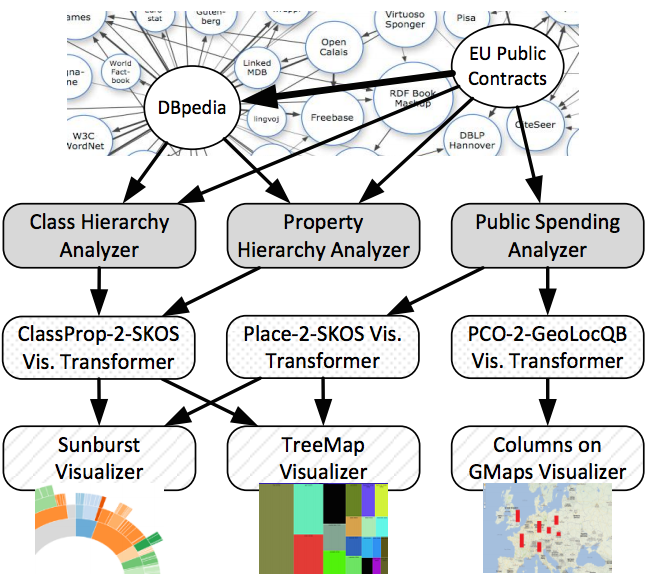
\includegraphics[scale=0.8]{img/ldvm-lod.png}
\label{fig:ldvm-lod}
\caption{Sample application of analyzers and visualizers in a LDVM pipeline.}
\end{figure}


\subsection{Discussion}
\label{sec:discussion}
There are currently many projects aiming at visualizing (RDF) Linked Data. A survey by Dadzie and Rowe \cite{Dadzie:2011} concluded with the fact that many visualization tools are not easy to use by lay users. In~\cite{Klimek2014} a recent review of some visualizations tools that can be summarized as follows:
\begin{itemize}
 \item \textit{Vocabulary-based visualization tools:} these tools are built for specific vocabularies and they help in visualizing data modelled according to those vocabularies, such as CubeViz \cite{cubeviz:2012}, FOAF explorer\footnote{\url{http://foaf-visualizer.gnu.org.ua/}} and Map4RDF \cite{leon2012}. They aim at visualizing data modelled respectively with \texttt{dq,foaf} and \texttt{geo+scovo}.
 \item \textit{Mashup tools:} they are used to create mashup visualizations with different widgets and some data analysis, such as DERI Pipes \cite{danh2009}. Mashup tools can be integrated into the LD wizard to combine different views of the data.
 \item \textit{Generic RDF visualization tools:} they typically support data browsing and entity rendering. They can also be used to build applications. In this category, we can mention Graphity\footnote{\url{https://github.com/Graphity/graphity-browser}}, lodlive\footnote{\url{http://en.lodlive.it/}} and Balloon Synopsis\footnote{\url{https://github.com/schlegel/balloon-synopsis}}.
\end{itemize}
While above-mentioned tools are often extensible and support specific domain datasets, they suffer from the following drawbacks:
\begin{itemize}
 \item \textit{They are not easy for lay users to set up and use}. Sometimes, users just need a visual summary of a dataset in order to start exploring the data. Our approach to this challenge is to provide such a lightweight JavaScript-based tool that supports a quick exploration task.
 \item \textit{They do not make recommendation based on categories}. A tool similar to our approach is Facete\footnote{\url{http://cstadler.aksw.org/facete/}}\cite{facete:2014} which shows a tree-based structure of a dataset based on some properties of an endpoint more relevant for geodata. A tabular view enables slices of data to be visualized and a map view can be activated when there is geodata. Our approach aims to be more generic, offering more views (tabular, map, graph, charts, etc.) based on a systematic analysis of the high-level categories present in a dataset.
\end{itemize}

The outcome of this state of the art can then be used to assess different visual tools in the process of creating Web-based visualizations. Some criteria can be used for assessing visual tools, such as (i) usability, (ii) visualization capabilities, (iii) data accessibility, (iv) deployment and (v) extensibility. In \cite{deliverable2012b}, the readers can find more details on this survey. Table \ref{tab:visuTools} gives an overview of the selected tools studied based on the following features:
\begin{itemize}
\item \textit{Data Formats} for the format of data taken as input by the tool;
\item \textit{Data Access}, for the way to access the data from the tool, such as Web service, SPARQL endpoint, etc.
\item \textit{Language code}, the programming language used to develop the tool;
\item \textit{Type of views}, the different views potentially accessible when using the tool;
\item \textit{Imported libraries}, the external libraries available within the tool,
\item \textit{License} for the Intellectual Property rights of the tool,
\item \textit{SemWeb compliant}, whether the tool can be easily extended or is compliant with structured data; and

\end{itemize}


\begin{landscape}
\begin{table}[htb!]
  \caption{Survey of tools used for creating visualizations on the Web.}
  \label{tab:visuTools}
  \centering
  \begin{tabular}{lccc}
    \toprule
    \textbf{Tools} & \textbf{Data Formats}& \textbf{Data Access} & \textbf{Language} \\
    \textbf{Views} & \textbf{Libraries} & \textbf{License} & \textbf{SemWeb App} \\
    \toprule
    \texttt{Choosel} & XLS, CSV & API & GWT \\
    Text/Map/Bar chart & Time (Simile)/Protovis/Flexvis & Open & No \\
    \midrule
    \texttt{Fresnel} & RDF & \-- & RDF \\
    Property/Labels & Welkin/IsaViz/Haystack/CSS & Open & Yes  \\
    \midrule
    \texttt{Spark} & RDF-JSON & SPARQL & PHP \\
    Charts/Tabular & \-- & Open & Yes \\
    \midrule
    \texttt{LDA} & RDF & SPARQL & Java/PHP \\
    \-- & \-- & Open & Yes \\
    \midrule
    \texttt{SemWeb Import} & RDF & SPARQL & Netbeans \\
    Graph Node & \-- &  CECILL-B & Yes \\
    \midrule
    \texttt{Many Eyes} & XLS/Text/HTML & API & Java/Flash \\
    Charts/Trees/Graphs/Maps & \-- & IBM & No \\
    \midrule
    \texttt{D3.js} & CSV/SVG, GeoJson & API & JavaScript \\
    Charts/Trees/Graphs/Maps & Jquery/sizzle/colorbrewer & Open & Maybe \\
    \midrule
    \texttt{Facet} & RDF-JSON & SPARQL & JavaScript \\
    Map, Facet view & JQuery/ dynatree &  Open & Yes \\
    \midrule
    Sgvizler & RDF-JSON & SPARQL & JavaScript \\
    Map/Line chart, Timeline/Sparkline & Google visualization API & Open & Yes  \\
    \midrule
    \texttt{Visual Box} & RDF & SPARQL & PHP/Django \\
    Map/Charts/ Timeline/Graphs & Google charts/TimeKnots/D3.js & Open & Yes  \\
    \midrule
    \texttt{Map4rdf} & RDF-JSON & SPARQL & Java/GWT \\
    Facet/Map & OSM Layers, Google Maps & Open & Yes \\
    \midrule
    \texttt{Exhibit} & JSON Exhibit & Data dump & JavaScript \\
    Map/Tile/Thumbnail/Tabular/Timeline & \-- & Open & Yes \\
    \midrule
    \texttt{Google Visualization API} & JSON/CSV & API & JavaScript \\
    Charts/ Charts/Maps/Dashboard & AJAX API & Open & Possible \\
    \bottomrule
  \end{tabular}
\end{table}
\end{landscape}

%\todo{Write here starting by "By contrast, our work ....}
\section{Describing Applications on the Web}
 \label{sec:descApps}

 \subsection{Motivation}
As many initiatives on Linked Open Data are growing, tools and technologies are getting more and more mature to help consumers to leverage the lifting process of the data. At the same times, standardization bodies such as the W3C are helping by providing best practices to publish Open Government Data by using appropriate vocabularies, taking care of stability in the URIs policies, and making links to other datasets. For instance the Government Linked Data Working Group\footnote{\url{http://www.w3.org/2011/gld/}} has released best practices and vocabularies to help governments publishing their data using Semantic Web technologies. Having a look at different proposals of the Life Cycle of Government Linked Data, one of the last stage is ``Publication'' where the data is released according to the 4-5 star principles\footnote{\url{http://5stardata.info/}}, with a given access to a SPARQL endpoint. However, for a better understanding of the data, one of the next steps is usually to generate visualizations through intuitive visual tools(charts, graphs, etc.) that will benefit to citizens, data journalists and other public authorities. Currently, one way of creating new applications is to look around previous initiatives to see what type of applications exist already and to make something similar according to a given dataset and domain. Another approach is by organizing \textit{contests} where the challenges are to mash up unexpected datasets with clear and beautiful visualizations. This approach is harder because developers also try figure out which tool and library is used for different applications. What if we describe applications according to the facets/views, datasets, visual tools used to build them? How are the types of information that can help create a vocabulary for annotating Web-based visualizations online?

\subsection{Catalogs of Applications}
We provide below two use cases of the current description of applications developed by datasets published on the Web. We expose also the limitation of the approach as they do not fully make use of semantics for improve discovery of the visual tools and datasets used to develop such applications.

\subsubsection{Open Data Service}
The Open Data Service at the University of Southampton\footnote{\url{http://data.southampton.ac.uk/apps.html}} has a register of all the applications developed using their datasets. A catalog of the Applications using the data is available at \url{http://id.southampton.ac.uk/dataset/apps}. Each application is described by giving three main categories of information:
\begin{enumerate}
\item The available distributions corresponding to the different formats HTML, RDF/XML and RDF/Turtle ;
\item Dataset information, which defines the type, the number of triples, license information, the publisher and the publication date.
\item The provenance, such as files used to generate the dataset for building the application, as well as the script itself.
\end{enumerate}



Currently, some vocabularies are used to model the catalog, such as the \texttt{DCAT} vocabulary \cite{dcat} and proprietary vocabularies. Each application is then described the type (Web, mobile Web, android, etc.), the authors, the date of creation and the datasets used to build the application. Figure \ref{fig:app-amenity} depicts the HTML view of a Web application
for a searchable map for finding buildings within the University sites. This initiative seems to be not extended. Thus, there is a real need to have a common layer of semantics for describing such applications. This would benefit the interoperability and discovery of applications on the Web.
\begin{figure}
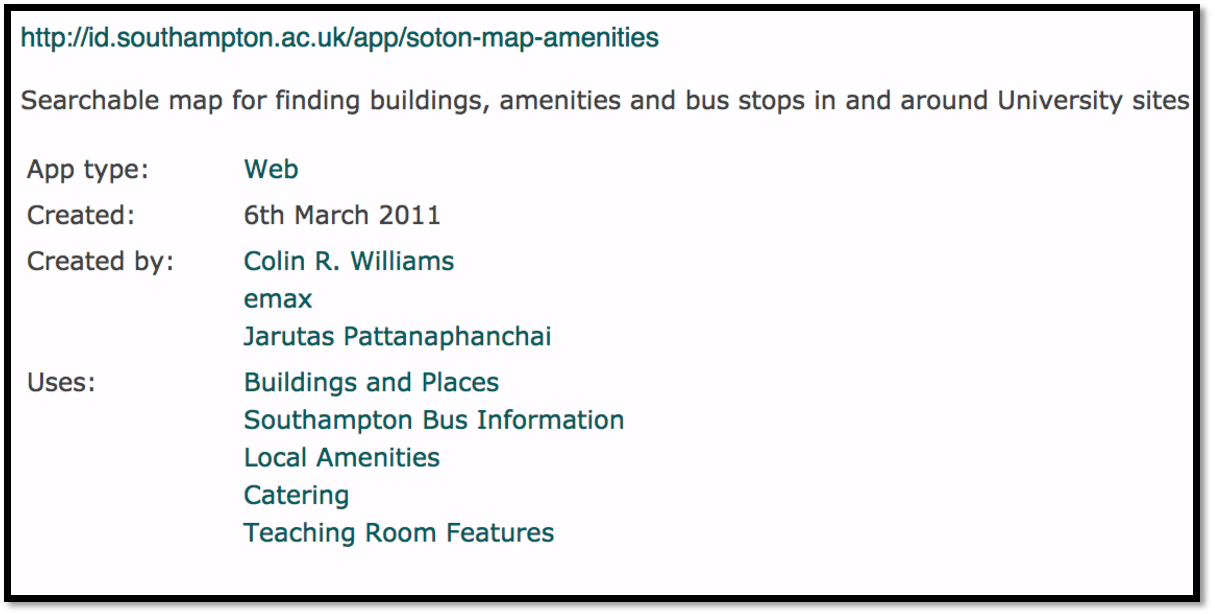
\includegraphics[scale=.7]{img/soton-map-amenities.pdf}
\label{fig:app-amenity}
\vspace{-10pt}
\caption{Sample description of a Web application  at the Open Data Service}
\end{figure}

\subsubsection{RPI Applications}
Another approach, taken by the researchers at the Rensselaer Polytech Institute\footnote{\url{http://data-gov.tw.rpi.edu}}, is to put at the bottom of the static page of a demo/application showcasing the benefits of Open Data for \texttt{data.gov}\footnote{\url{https://www.data.gov/}} some basic metadata (description, URL to dataset, author), and also a link to the SPARQL query used for generating the application. As this information is human-readable and can help, the main drawback is the lack of a machine-readable version, using semantics to discover and connect different demos and datasets with authors. A more vocabulary can leverage the issue by annotating such applications to help discovering and aggregating other similar applications in other Open Data initiatives.


\section{Describing and Modeling Applications}
\label{sec:apps}
According to \cite{card99}, \texttt{Visualization} is \textit{ ``the use of computer-supported, interactive visual representations to amplify cognition''}. So the unique object of visualization is to develop insights from collected data. That explains why each time a new dataset is released, users always expect some showcases to play with the underlying datasets. It is true that many public open initiatives use incentives actions like \textit{challenges}, \textit{datahack-day} or \textit{contest}, etc. to find innovative applications that actually exhibit the benefits of datasets published. Visualizations play crucial role as they can easily find errors in a large collection, detect patterns in a dataset or help navigate through the dataset.

\subsection{Typology of Applications}
Jeni Tennison defines  in her blog\footnote{\url{http://www.jenitennison.com/blog/node/126}} three categories of applications using online data:
\begin{itemize}
\item (i) \textit{data-specific applications}, which are constructed around particular data sets that are known to the developer of the application; hence the visualizations obtained are of data-specific applications. Examples are the famous applications of \textit{``Where does my money go''}  in Greece\footnote{\url{http://publicspending.medialab.ntua.gr/en/index.php}} or the UK\footnote{\url{http://wheredoesmymoneygo.org/}}. Those applications are also called \textit{``mashups''}.
\item (ii) \textit{vocabulary-specific applications}, which are constructed around particular vocabularies, wherever the data might be found that uses them. Examples here are the FaceBook Social Graph API\footnote{\url{https://developers.facebook.com/docs/plugins/}} and IsaViz  \cite{isaviz}, among others.
\item (iii) \textit{generic applications}, which are constructed to navigate through any RDF that they find; e.g., Tabulator \cite{tabulator06}, OpenLink Data Explorer\footnote{\url{http://ode.openlinksw.com/}}.

\end{itemize}
Because most mash-ups are data-specific applications, it is important to  know what information the dataset contains. This could be achieved by giving the meaning of some properties or classes of the vocabularies used to create the dataset. Hence, what the data publisher very often needs to do is to make sure that the data they publish is documented. However, what is used in practice, is to consider using an intuitive visualization self-descriptive to both show the added-value of the data and its documentation.

\begin{table}[ht!b]
    \caption{Gathering reusable information from the openspending in Greece application} \label{tab:describeApps}
    \small
    \center
    \begin{tabularx}{\textwidth}{@{}lX@{}}
     %\begin{tabular}{@{}llX@{}}
    \toprule
    \textbf{Features} & \textbf{Value}\\
    \toprule
    \texttt{Access Url }&	\url{http://publicspending.medialab.ntua.gr/}\\
    \midrule
    \texttt{Scope/Domain} &	Public spending, Government \\
    \midrule
    \texttt{Description} & The application helps visualizing the most characteristic facts of the Greek public spending, interconnected to foreign expenditure and other data. \\
    \midrule
    \texttt{Supported Platform} &	Web \\
    \midrule
    \texttt{URL Policy}   &  http://{BASE}/en/{NAME-CHART}.php e.g., \url{http://{BASE}/en/toppayersday.php} \\
    \midrule
    \texttt{Data Source}	& \url{http://opendata.diavgeia.gov.fr}; Greek Tax data (TAXIS) \\
    \midrule
\texttt{Type of views} & Bubble tree, column and bar charts \\
    \midrule
   \texttt{Visualization tools} &  HighchartsJS,  Bubble TreeJS JqueryJS ; RaphaelJS \\
   \midrule
  \texttt{License} & Open \\
    \midrule
\texttt{Business Value} & Not Commercial (Free) \\
    \bottomrule

    % \end{tabular}
    \end{tabularx}
    \end{table}

\subsection{Reusable applications} \label{sec:reusable}
%\todo{ summary of the application survey D6.1: diversity, scope, and countries}
Many applications are built on top of datasets exposed in different open data governments initiatives. Generally, they are used to provide insight about the datasets and their usefulness. However, some of the applications could be generalized and reused if published adequately. Having some best practices in publishing applications on the Web could boost the interoperability between datasets and visual tools. To achieve this task, we first review some applications that have been developed on top of datasets  opened by governments (UK, USA, France) and public local authorities. We made a random survey of thirteen (13) innovative applications \cite{deliverable2012a} in various domains such as of security, health, finance, transportation, housing, city, foreign aid and education. Table \ref{tab:apps-survey} provides a summary of the surveyed applications; with names, types, countries and brief description.

The main template used in the survey gathered the following information:
\begin{itemize}
\item the name of the application;
\item the scope or the target domain of the application;
\item a small and concise description;
\item the platform on which the application can be deployed and view;
\item the policy used for creating the URL of the application;
\item the legacy data used to build the application, and a mention of the process of the ``lifting process'' of the raw data to RDF if available;
\item the different views available from the application;
\item comments or relevant drawbacks;
\item the license of the application.
\end{itemize}
 Table \ref{tab:describeApps} provides the information extracted from \texttt{openspending in Greece} using the aforementioned template. Such information can be published using a vocabulary to help discover all the applications built on top of public spending data across different platforms.




% \section{Evaluating Visualizations}
% See Roberto Garcia work and proposal in Datalift technical report.


\begin{table}[ht!b]
    \caption{Some innovative applications buit over Open Government Datasets} \label{tab:apps-survey}
    \small
    \center
   \begin{tabularx}{\textwidth}{@{}llllX@{}}
    % \begin{tabular}{@{}llX@{}}
    \toprule
    \textbf{Application} & \textbf{Domain} & \textbf{Type} &  \textbf{Country}  \\
    \toprule
    \texttt{UK Crime} &	Crimes & Web & UK  \\
    \midrule
\texttt{UK Pharmacy} & Health, Pharmacy  & Mobile/Android  & UK \\
	\midrule
	\texttt{Numberhood} & Local area dynamics  & iPhone/iPad & UK \\
	
	\midrule
	\texttt{BuSit London} & Public Transportation  & Web and mobile  & UK \\
	
	\midrule
	\texttt{UK School Finder} & Education  & Web  & UK \\
	
	\midrule
	\texttt{Where-can-I-Live} & Homes, Transportation & Web  & UK \\
	\midrule
	
	\texttt{Opendatacommunities} & Local Government & Web  & UK \\
	\midrule
	
	\texttt{FlyOnTime } & Flights/airlines & Web  & USA \\
	\midrule
	
	\texttt{White House Visitor Search} & White House & Web  & USA \\
	\midrule
	
	\texttt{US-USAID/UK-DFID} & Foreign aid & Web  & USA \\
	\midrule
	
	\texttt{Fourmisante} & Medicine/Health-care & Web  & France \\
	\midrule
	
	\texttt{MaVilleVueDuCiel} & Local Government  & Web & France \\
	\midrule
	
	\texttt{Home'n'Go } & Housing & Web & France \\
	
	
    \bottomrule

    %\end{tabular}
    \end{tabularx}
    \end{table}

 \subsection{A vocabulary for Describing VIsualization Applications} \label{sec:dvia}

We have implemented a vocabulary, DVIA\footnote{\url{http://bit.ly/Vb4L8k}}, that aims to describe any applications developed to consume datasets in compliant with 4-5 stars rate, using visual tools to showcase the benefits of Linked Data. It reuses four existing vocabularies: Dublin Core\footnote{\url{http://purl.org/dc/terms/}}, dataset catalogue (DCAT)\footnote{\url{http://www.w3.org/ns/dcat\#}}, Dublin Core Metadata Initiative\footnote{\url{http://purl.org/dc/dcmitype}} and the Organization vocabulary \footnote{\url{http://www.w3.org/ns/org\#}}.  It is composed of three main classes:

\begin{itemize}
\item \textbf{Application}: This class represents the application or the mashup developed for demoing or consuming data in LD fashion. It is a subclass of \textbf{dctype:Software}
\item \textbf{Platform}: The platform where to host or use the application, could be on the Web (Firefox, Chrome, IE, etc..) or mobile (android, iOS, mobile ) or even desktop
\item \textbf{VisualTool}: Represents the tool or library used to build the application.
\end{itemize}

Figure \ref{visuGraphModel} depicts the model used to implement the DVIA vocabulary.

\begin{figure}[!htbp]
\vspace{-2.5cm}
  \centering{
    %\leavevmode
      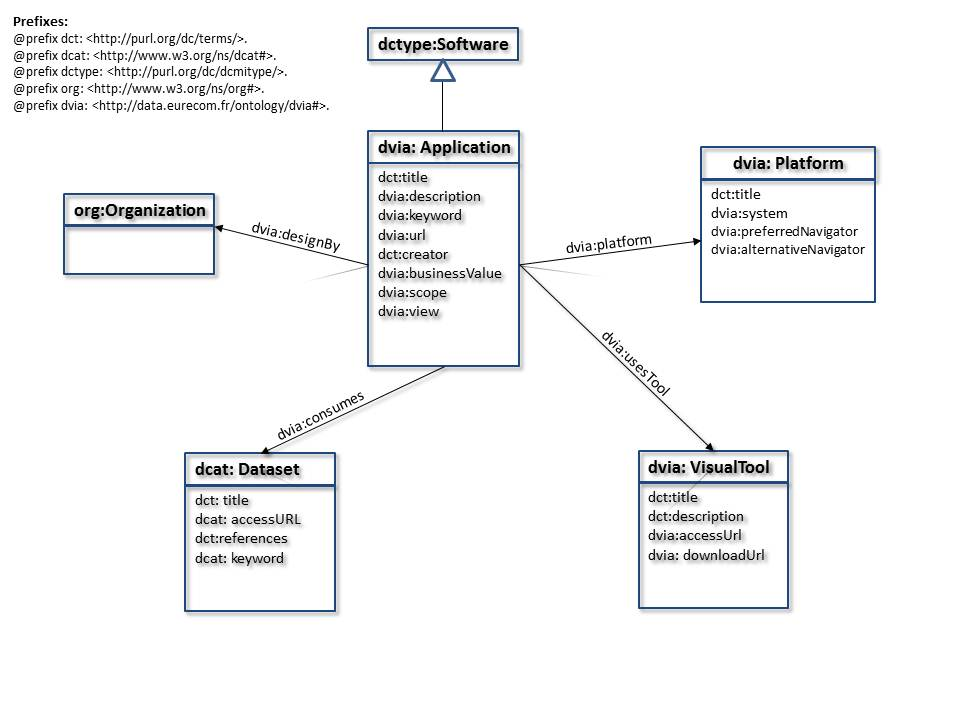
\includegraphics[ height=5in]{img/visuGraphModel.jpg}

    \caption{Conceptual Model of the DVIA vocabulary }
    \label{visuGraphModel}
  }
\end{figure}

The main classes and properties are depicted in Figure \ref{visuGraphModel}. The current version of the vocabulary in Turtle format can be found at \url{http://purl.org/ontology/dvia} .  Listing \ref{snapshotEventMedia} is a snapshot of the description of \textit{EventMedia Live}\footnote{\url{http://challenge.semanticweb.org/2012/winners.html}} application in DVIA. It depicts apart from some metadata about the application (dct:title, dct:name, dct:issued, dct:creator and dct:license), the different visualization libraries integrated for building EventMedia Live (e.g. The Google API, Backbone, etc), as well as the operating systems where it is designed for, the different views/facets available in the application (map, charts, graphs, force-directed layout, etc.) and the heterogeneous datasets used to implement it.

\lstset{basicstyle=\scriptsize, backgroundcolor=\color{white}, frame=shadowbox, caption= {Snapshot in Turtle of the description of Event Media Live Application}, label=snapshotEventMedia, captionpos=b}
\begin{lstlisting}
visuapp:eventMedia01
   a dvia:Application ;
   dct:title "EventMedia Live"@en;
   dvia:description "An application for reconciling Live events with media" ;
   dvia:url <http://eventmedia.eurecom.fr> ;
   dct:issued "2012-11-10"^^xsd:date ;
   dvia:businessValue "not commercial" ;
   dvia:keyword "events, media"^^xsd:string ;
   dct:license <http://www.opendatacommons.org/licenses/pddl/1.0/> ;
   dvia:platform [ a dvia:Platform ;
      dct:title: "Desktop" ;
	  dvia:preferredNavigator "Google Chrome" ;
	  dvia:alternativeNavigator "FireFox" ;
	  dvia:system "Mac OS, Windows, Linux"^^string ] ;	
   dvia:usesTool [ a dvia:visualTool; 
      dct:title "Google visualization Tool" ;
	  dct:description "Google visualization API" ;
	  dvia:accessUrl <https://developers.google.com/chart/interactive/docs/reference> ;
	  dvia:downloadUrl <http://www.google.com/uds/modules/gviz/gviz-api.js/> ] ;
   dvia:usesTool visuapp:visualTool02 ;
   dvia:consumes [ a dcat:Dataset; dct:title "BBC dump"] ;
   dvia:consumes [ a dcat:Dataset; dct:title "last.fm scrapped dataset"] ;
   dvia:consumes [ a dcat:Dataset; dct:title "upcoming scrapped dataset"] ;
   dvia:consumes [ a dcat:Dataset; dct:title "eventful scrapped dataset"] ;
   dvia:consumes [ a dcat:Dataset; dct:title "Flickr scrapped dataset"] ;
   dvia:consumes [ a dcat:Dataset; dct:title "Music Brainz "] ;
   dvia:consumes [ a dcat:Dataset; dct:title "Foursquare Json file"] ;
   dvia:consumes [ a dcat:Dataset; dct:title "DBpedia"] ;
   dct:creator [foaf:mbox "khrouf@eurecom.fr"; foaf:name "Houda Khrouf"];
   dct:creator [foaf:mbox "vuk@eurecom.fr"; foaf:name "Vuk Milicik"];
   dct:creator [foaf:mbox "raphael.troncy@eurecom.fr"; foaf:name "Raphael Troncy"];
   dvia:view "map, chart, graph, force-directed layout" ;
   ...
\end{lstlisting}

The full version of this sample description is available at \url{http://www.eurecom.fr/~atemezin/datalift/visumodel/eventMedia-sample.ttl}. The current version of the DVIA intends to be small enough to cover the concepts that are needed to reuse partial or full parts of applications.

\section{Summary}
In this chapter, we have described different tools used for visualizing data, structured and graph data. We have also discussed different types of applications currently built on top of government open data initiatives. The goal of this survey is to propose some new approaches of generating and discovering visualizations and applications on the Web of Data. We designed and implemented DVIA, a vocabulary that aims to model applications for more interoperability and discovery of applications and tool visualizations on the Web.

\clearpage

\chapter{New Approaches for Generating Visualizations and Applications}
\label{ch:ch5}

\begin{flushright}
\textit{``A Semantic Web application is one whose schema is expected to change.''} \\ (David Karger, MIT CSAIL)\footnote{A statement during his keynote at ESWC 2013 conference}
\end{flushright}


\section{Introduction}
\label{sec:introch5}

Linked data offers some great advantages for publishing government data. The approach makes it easy to publish information in a way that allows it to be combined with other sets of data. The benefits also arise from the semantics associated to things, common identifiers for things, from the inherent extensibility of the RDF data model, and from the publication of data in a standard format. Linked data is a great way of publishing information for diverse and distributed organizations, such as government \cite{tennison10}.  

However, the RDF model, its various serializations and the SPARQL query language are foreign to the majority of developers. Those developers understandably want to be able to use the tool chains that they are familiar with to access government data. Publishing data purely as RDF, and providing access purely through SPARQL queries raises an unacceptable barrier onto the use of that data. 

\textcolor{red}{Steps for creating a visualization over RDF from scratch: 
-------
To create a web-based visualization from scratch, the user should need to know how to do several tasks. First, the user should know how to write a program to send the query to a SPARQL endpoint, obtain the results and process them properly. Second, the user should need advanced knowledge in a programming language such as JavaScript or Flash, along with other languages such as Cascade-style sheet (CSS), Scalable Vector Graphics (SVG)[48] and other web technologies. In many cases this is not enough, and knowledge related to libraries such as the ones mentioned in Section 2.2 would be necessary as well. Third, all these tasks need to be done separately, since no integrated environment is used. Thus, the main advantage of Visualbox is that it reduces the knowledge necessary to create a visualization and diminish the complexity of the project by helping performing these tasks in one integrated environment.}


\section{Wizard for Visualizations}

%\ghis{find a good justifying example} \\

With the growing adoption of the Linked Data principles, there is a real need to support data consumers in quickly getting visualizations that enable to explore a dataset. In order to involve more general Web users into the Semantic Web and Linked Data world, there is a need to build tools that reuse existing visualization libraries showing the key information about RDF datasets. Many datasets are published using SPARQL Endpoints and are not ``visually'' accessible. Thus, understanding the underlying graphs and consuming them require lay users to have some knowledge in writing queries. 

The object of visualization is to develop insights from collected data. Moreover, according to Information Theory, vision is the sense that has the largest bandwidth (100 Mbits/s), which makes it the best suited channel to convey information to the brain \cite{Ware:2014}. Based on the Visual Information Seeking Mantra: \textit{``overview first, zoom and filter, then details on demand''} \cite{Shneiderman99}, we advocate for more visual interactive representations of RDF graphs using SPARQL Endpoints.   At the same time,  we use the term ``Linked Data Visualization'', to refer to a \textit{combination of charts, graphics, and other visual elements built on top of 4-5 stars datasets accessible via a SPARQL endpoint}. 
Despite the presence of more and more datasets published as Linked Data, there is still a need to help end users to discover what (unknown) datasets describe by hiding the complexity of SPARQL queries from such users. Moreover, the task of identifying the key categories of datasets can help in selecting and matching the most suitable visualization types.

In this Section, we propose a first step towards making available a semi-automatic way for the production of possible visualization of linked data sets of high-level categories grouping objects that are worth viewing and we associate them with some very well known vocabularies. Then, we describe the implementation of a Linked Data Visualization Wizard and its main components. This wizard can be used to easily visualize slices of datasets based on generic types detected.

The remainder  of this paper is structured as follows. We first provide some related work that further motivates this study (Section~\ref{sec:related}). In Section~\ref{sec:vizTypes}, we propose some important categories that are worth visualizing and we present a set of mapping views associated with vocabularies (Section~\ref{sec:mapping}). In Section~\ref{sec:ldvizwiz}, we describe the implementation of a wizard that can work on top of any RDF dataset. We detail the results of an experiment where high level categories and associated visualizations have been performed on numerous SPARQL endpoints (Section~\ref{sec:evaluation}). 

\subsection{Dataset Analysis}
\label{sec:vizTypes}
When developing an application, there are some ``important'' classes/categories, objects or datatypes that can be detected first to help to guide in the progress of creating a set of visualizations tied with those categories. We distinguish seven categories while acknowledging that this is not necessary an exhaustive list:
\begin{itemize}
 \item{\S~[\textbf{Geographic information}]}: This category is for data modeled using \texttt{geo:SpatialThing}, \texttt{dbpedia-owl:Place}, \texttt{schema:Place} or \texttt{gml:\_Feature} classes.
 \item{\S~[\textbf{Temporal information}]}: This category also includes dataset containing date, time (e.g: \texttt{xsd:dateTime}) and period or interval of time, using the OWL Time ontology.
 \item{\S~[\textbf{Event information}]}: This category is for any action of activity occurring at some place at some time.
 \item{\S~[\textbf{Agent/Person information}]}: This category is heavily influenced by the use of \texttt{foaf:Person} or \texttt{foaf:Agent}.
 \item{\S~[\textbf{Organization information}]}: This category is related to organizations or companies data, with the use of the \texttt{org} vocabulary\footnote{\url{http://www.w3.org/TR/vocab-org/}} or the \texttt{foaf:Organization} class.
 \item{\S~[\textbf{Statistics information}]}: This category refers to statistical data generally modeled using the \texttt{data cube} vocabulary\footnote{\url{http://www.w3.org/TR/vocab-data-cube/}} or the SDMX model\footnote{\url{http://sdmx.org/}}.
 \item{\S~[\textbf{Knowledge Classification}]}: This category refers to dataset describing schemas, classifications or taxonomies using the \texttt{SKOS} vocabulary.
\end{itemize}



\section{Mapping Datatype, Views and Vocabularies}
\label{sec:mapping}
%\todo{add ref. to "Interactive Data Visualization" by Ward et al.}

The On-line Library of Information Visualization Environments (OLIVE)\footnote{\url{http://lte-projects.umd.edu/Olive/}} is a web site describing eight categories of information visualization environments differentiated by data type and collected by students, following a visualization course given at Maryland College Park, mostly inspired from the work of Ben Shneiderman \cite{Shneiderman99}. Based on the classification provided by OLIVE, we propose a set of mappings between those categories (excluding the workspace dimension), views that can be applied to this category and a suitable list of vocabularies from the Linked Open Vocabularies catalogue \cite{lov11}\footnote{\url{lov.okfn.org/dataset/lov/}} that correspond to those categories. Those vocabularies are easy to be found as there is a manual classification of vocabularies by the curators of the catalogue based on the content and scope of the terms and properties. According to the seven categories defined in Section ~\ref{sec:vizTypes}, we have identified some of their corresponding one to one mapping with the set of vocabularies:
 \begin{itemize}
 \item \textbf{Geography} space, consisting of 21 vocabularies for features: \texttt{geo}, \texttt{gn}, \texttt{gf}, \texttt{om}, \texttt{geop}, \texttt{md}, \texttt{lgdo}, \texttt{loc}, \texttt{igeo}, \texttt{osadm}, \texttt{geod}, \texttt{ostop}, \texttt{place}, \texttt{geos}, \texttt{locn}, \texttt{coun}, \texttt{postcode}, \texttt{osr}, \texttt{geof}, \texttt{g50k} and \texttt{ad}.
 \item \textbf{Geometry} space, for vocabularies dealing with the geometries, mostly combined with the features, such as: 
 \item \textbf{Time} space, consisting of 14 vocabularies, such as \texttt{cal}, \texttt{date}, \texttt{gts}, \texttt{interval}, \texttt{ncal}, \texttt{oh}, \texttt{te}, \texttt{thors}, \texttt{ti}, \texttt{time}, \texttt{tl}, \texttt{tm}, \texttt{tvc} and \texttt{tzont}. 
 \item \textbf{Event} space, containing vocabularies such  as \texttt{event}, \texttt{lode}, \texttt{music}, \texttt{sem}, \texttt{situ}, \texttt{sport}, \texttt{stories}, \texttt{theatre}, \texttt{tis} and \texttt{tisc}.
 \item \textbf{Government} space, with 9 vocabularies (\texttt{cgov}, \texttt{ctorg}, \texttt{elec}, \texttt{few}, \texttt{gc}, \texttt{gd}, \texttt{oan}, \texttt{odd}, \texttt{parl}) and the \texttt{org} vocabulary belonging to the W3C recommendation vocabularies at \url{ http://lov.okfn.org/dataset/lov/lov#W3C}.
 \end{itemize} 
 Metadata vocabularies, such as \texttt{rdfs}, \texttt{dcterms} or \texttt{dce} can be used in association with any of the visual element to give basic description of the resource of a giving dimension. For example, a popup information can be fired on a map view to display the relevant information of a geodata resource such as the label, the abstract or description. 
Another application can be to detect which visualization is best suited for geodata. Geodata belongs to a  two-Dimension visual representation. Geodata is usually displayed using geographical-based visualizations (map, geo charts, etc.) and it is often modeled by vocabularies in the space named \texttt{Geometry} and \texttt{Geography}\footnote{All the prefixes used for the vocabularies are the same used in LOV catalogue.}   vocabularies in RDF datasets. Hence those vocabularies can be combined to detect the presence or not of geographic information in a dataset, and thus yield to recommend a map view. Table~\ref{tab:taxonomy} gives an overview of those mappings. For the tabular representation, it is the ``default'' visual representation of RDF data and can be used by any vocabulary without restriction. 


\begin{table}[!htbp]
\centering{
\begin{tabular}{lllc}
 \specialrule{1pt}{1pt}{1pt}
 \textbf{Dimension}	 	& \textbf{Vocabulary Space}  & \textbf{Visual element}		 \\ \specialrule{1pt}{1pt}{1pt}
 Temporal 	     &  \textsf{Time space} &     TimeLine		      	 		 \\
 one-Dimension  & \textsf{any}	   & Tabular, text							 \\
 two-Dimension   & \textsf{Geography space}     & Map view 						\\
 			& \textsf{Geometry space}    & Maps view                            \\
 three-Dimension  	& \textsf{Event space}  	& Map + TimeLine	 			\\
 Multi-Dimension  & \textsf{qb}, \textsf{sdmx-model}, \textsf{scovo}      & Charts, graphs   			 		\\
 Tree	      &   \textsf{skos, Government space}            & Treemap, Org view   				\\
 Network	  & \textsf{any vocab.}   & Graph, network map  			 			
 \\
 \specialrule{1pt}{1pt}{1pt}
\end{tabular}
\caption{A taxonomy of information visualization consuming Linked Datasets with associated views and suitable vocabulary space.}
\label{tab:taxonomy}
}
\end{table}


\section{LDVizWiz: a Linked Data Visualization Wizard}
\label{sec:ldvizwiz}

%\todo{present in detail the queries for detecting ALL the categories} \\

We propose a workflow composed of four principal steps for a Linked Data Visualization Wizard, as depicted in Figure~\ref{fig:workflow}. Our requirement is to provide a tool that hide the complexity of SPARQL to lay users and at the same time, can be embedded in existing Linked Data infrastructure and workflow. First, we proposed to detect the presence of data belonging to one of the seven categories (Table~\ref{tab:taxonomy}) using generic SPARQL queries. More precisely, we perform \texttt{ASK} queries to test whether or not a particular query pattern has a solution. Second, we look at entities in a dataset that have \texttt{owl:sameAs} links with external objects and we retrieve the properties associated to those objects. We argue that the objects that are interlinked with other datasets are of primary importance in a visualization. We show the results of this mining process to the user (the categories that have been detected, the properties going with the categories and the external domain). Based on this information, the user can make a personalized ``mashup'' by aggregating the suitable visualization widgets. Some default visualizations are available according to the top categories detected. The last step is to publish the visualization and a metadata report in RDF/XML TURTLE or N3.

\begin{figure*}[!htbp]
\begin{center}
\subfigure[The workflow of the different modules interacting in the Linked Data visualization wizard.]{
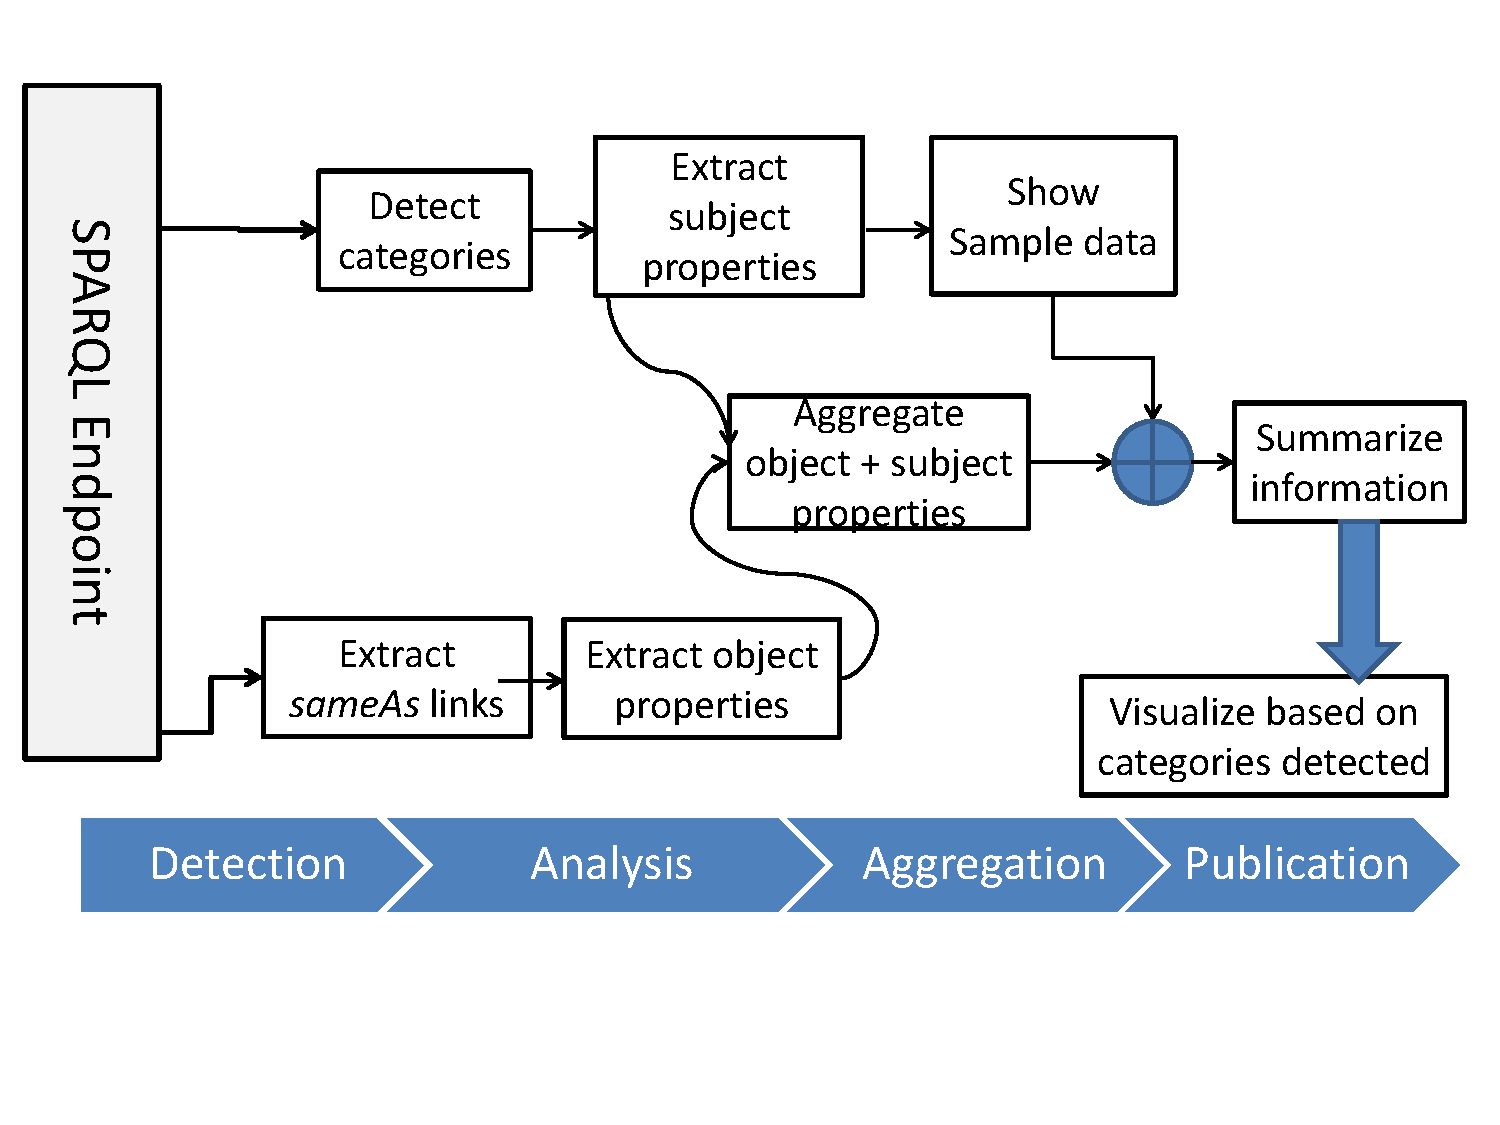
\includegraphics[width=0.5\textwidth]{img/workflow-visu.pdf}
}
\subfigure[High level functionalities of the Linked Data visualization wizard ]{
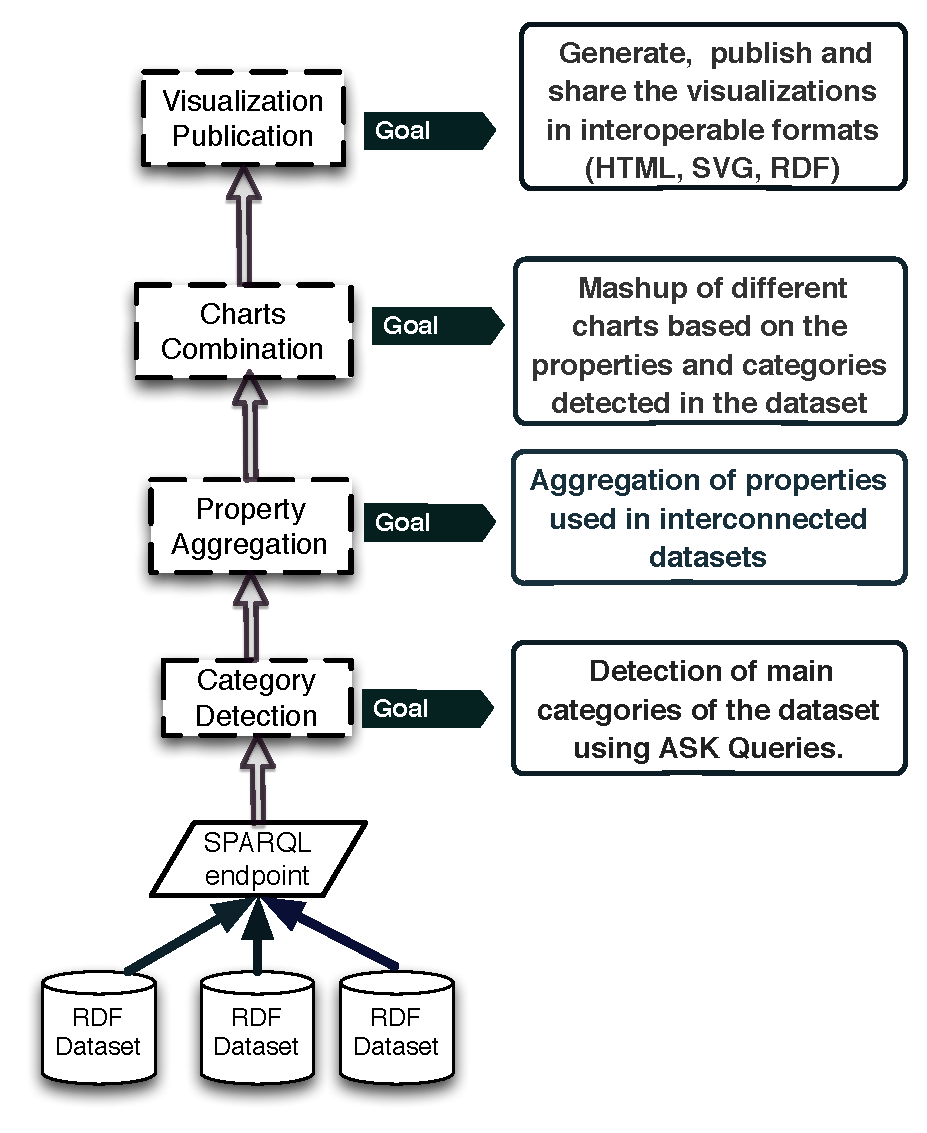
\includegraphics[width=0.4 \textwidth]{img/architecture-ldwizard.pdf}
}


\caption{Big picture and architecture of the Linked Data visualization wizard.}
\label{fig:workflow}
\end{center}
\end{figure*}

Let consider a graph $<G,c>$ to be $G=\{(s,p,o)| p \in URI, s \in URI, o \in (URI \cup LIT)\} $ where $URI$ is the set of URIs, $LIT$ is the set of literals, and $c$ the context. We define $L=\{V_{1}, V_{2}, ...,V_{n} | V_{i}=P_{i} \cup T_{i}\} $ the list of vocabularies in LOV, with $P_{i}$ and $T_{i}$ respectively the properties and terms of a vocabulary $V_{i}$. Let also $D=\{D_{1}, D_{2}, ..,D_{m} \} $ be the domains of vocabularies. We assume $ \forall V \in L, \exists D_{k} \in \Phi(L,D) $. We define a generic function $\Sigma:(G,c)\mapsto B $ to detect categories in a dataset as follows: $\Sigma((G,c))=\{B| ( \exists(s,p,o) \in G: p \in V) \cup (\exists(s, rdf:type,o) \in G: o \in V)\} $ where $B =\{True, False\} $.


In the following sections, we describe each of the steps involved in the Linked Data Visualization Wizard in more details. 

\subsection{Category Detection}
The goal of the category detection task is to use SPARQL queries to detect the presence of some high level categories in the dataset. We perform \texttt{ASK} queries as implementation of the $\Sigma $ function using standard vocabularies as defined in the Table~\ref{tab:taxonomy}. We start with six categories, namely: geographic information, person, organization, event, time and knowledge organization systems. We select popular vocabularies based on two existing catalogues: LOV~\cite{pyv2012} and prefix.cc\footnote{\url{http://prefix.cc}}.

%asking geodata
\lstset{basicstyle=\scriptsize, backgroundcolor=\color{white}, frame=single, caption= {Generic query to detect geo data from a SPARQL endpoint}, label=geodata, captionpos=b}
\begin{lstlisting}
ASK WHERE {
 {
  ?x a ?o.
  filter (?o= dbpedia-owl:Place ||
    ?o=gml:_Feature || 
    ?o=geo:SpatialFeature || ?o=gn:Feature ||
    ?o=admingeo:CivilAdministrativeArea ||
    ?o=spatial:Feature ||
    ?o=vcard:Location)
 }
 UNION {
  ?x ?p ?o. filter(?p=geo:lat || ?p=geo:long ||
  ?p=georss:point || ?p=geo:geometry || 
  geom:geometry)
 }
}
\end{lstlisting}

 Listing~\ref{geodata} shows seven classes of different vocabularies are used, respectively for the namespaces \texttt{dbpedia-owl, geo, gn, admingeo, spatial} and \texttt{vcard}, with relevant classes to check the presence of geographic data.

\lstset{basicstyle=\scriptsize, backgroundcolor=\color{white}, frame=single, caption= {Generic query to detect time data from a SPARQL endpoint, using \texttt{time, dbpedia-owl, intervals} vocabularies.}, label=timedata, captionpos=b}
\begin{lstlisting} 
	ASK WHERE {{?x a ?o. filter(?o=time:TemporalEntity || 
	?o=time:Instant || 
		?o=time:Interval || ?o=dbpedia-owl:TimePeriod || 
		?o=time:DateTimeInterval || ?o=intervals:CalendarInterval)
	} 
	UNION{ ?x ?p ?o. filter(?p=time:duration || 
	?p=time:hasBeginning || 
	?p=time:inDateTime || ?p=time:hasDateTimeDescription 
	|| ?p=time:hasEnd)}

\end{lstlisting}

Listing \ref{timedata} detects the presence of time information, while Listing \ref{persondata}, \ref{orgdata} and \ref{eventdata} detect persons, organizations and events respectively.

\lstset{basicstyle=\scriptsize, backgroundcolor=\color{white}, frame=single, caption= {Generic query to detect person categories from a SPARQL endpoint, using \texttt{foaf, dbpedia-owl, vcard} vocabularies.}, label=persondata, captionpos=b}
\begin{lstlisting}
	ASK WHERE {?x a ?o. filter(?o = foaf:Person ||
	 ?o=dbpedia-owl:Person ||
		?o=vcard:Individual) }
	
\end{lstlisting}

\lstset{basicstyle=\scriptsize, backgroundcolor=\color{white}, frame=single, caption= {Generic query to detect ORG data from a SPARQL endpoint.}, label=orgdata, captionpos=b}
\begin{lstlisting}
PREFIX org:<http://www.w3.org/ns/org#>
	PREFIX foaf: <http://xmlns.com/foaf/0.1/> 
	PREFIX dbpedia-owl: <http://dbpedia.org/ontology/> 
	ASK WHERE {?x a ?o . filter (?o=org:Organization || 
	?o=org:OrganizationalUnit || 
	?o=foaf:Organization || 
	?o=dbpedia-owl:Organisation)}
	
\end{lstlisting}	

\lstset{basicstyle=\scriptsize, backgroundcolor=\color{white}, frame=single, caption= {Generic query to detect event data from a SPARQL endpoint, using \texttt{lode, event, dbpedia-owl} vocabularies.}, label=eventdata, captionpos=b}
\begin{lstlisting}
    ASK WHERE{?x a ?o. filter (?o= lode:Event || ?o=event:Event || 
    ?o=dbpedia-owl:Event)}	
    
  \end{lstlisting}
  
  
For detecting data organized as taxonomy, \texttt{skos} vocabulary is used along with the most used classes and properties as showed in Listing \ref{skosdata}.

\lstset{basicstyle=\scriptsize, backgroundcolor=\color{white},
frame=single, caption= {Generic query to detect SKOS data from a SPARQL endpoint, using \texttt{skos} vocabulary.}, label=skosdata, captionpos=b}
\begin{lstlisting}
    ASK WHERE {{?x a ?o. filter(?o=skos:Concept ||
     ?o=skos:ConceptScheme || ?o=skos:Collection )}
    	 UNION{ ?x ?p ?o. filter(?p=skos:featureCode || 
    	?p=skos:altLabel || ?p=skos:prefLabel  || ?p=skos:relatedMatch)}}		
\end{lstlisting}


\subsection{Property Aggregation}
We take the benefits of the \texttt{owl:sameAs} links between entities to have access to the properties of the entities in the external namespaces different from the origin dataset. This module also aggregates the properties found in the dataset with the ones found in the interlinked sets. This is based on the assumption that during the linkage process, external datasets not only help in not breaking the \textit{follow-your-nose} principle, but also add more information to be viewed in visualization applications. As shown in the code below, at this stage, we have collected and aggregated external properties gathered from the enrichment process of the workflow.

\begin{verbatim}
1-LET Namespace(?s) = S and LET Namespace(?t) =T
2-SELECT  owl:sameAs links
	LET SEMTERM = list of ?s owl:sameAs ?t
	WITH T != S
3-IN T, SELECT distinct properties used in dataset
4-AGGREGATE (3) with properties FROM S.
\end{verbatim}

\subsection{Visualization Generator}
This module aims at recommending the appropriate visualizations based on the categories detected by the wizard. It might also help the user to make a report summarizing the result of the mining process, and then use different visualization libraries to view the data. This module can be viewed as a recommender system because it derives visualizations based on the categories. The input to build each visualization is the corresponding SELECT query of each ASK queries used to detect the categories. Moreover, some adjustment are made to avoid blank nodes and to get the labels of the resources. The generator can be coupled with a mashup widget generator for some  categories. For example, users could expect for event data, a combination of map view (where), a timeline (when) and facets based on the agents (who).

\subsection{Visualization Publisher}
The publisher module aims at exporting the combined visualizations, along with the report of all the process of mining the dataset, in a format easy to share, either as HTML, SVG or in the different RDF syntax flavor. For the latter, apart from using metadata information (creator, issued date, license), we model the categories we have detected using the \texttt{dcterms:subject} property of a \texttt{dcat:Dataset}, the queries used (using the \texttt{prov:wasDerivedFrom} property), the sample resources for each category (using the \texttt{void:exampleResource} property) and the visualization generated (using the \texttt{dvia} and \texttt{chart}\footnote{\url{http://data.lirmm.fr/ontologies/chart}} vocabularies).

\section{Experiment and Implementation}
\label{sec:evaluation}
In this section, we describe the experiments and report the evaluation on detecting categories on 444 endpoints. We then describe a prototype as a ``\texttt{proof-of-concept}'' of the proposal. 

\subsection{Experiment set up}
%\todo{explain and discuss in detail the experiment} \\
We have evaluated our approach on the list of $444$ endpoints referenced at \url{http://sparqles.okfn.org/} monitoring the availability, performance, interoperability and discoverability of SPARQL Endpoints registered in Datahub \cite{buil2013} . We have implemented a script in python to speed up the process and obtain the results. Every ASK query for the different category is implemented in a separate function requesting a JSON response.
 

\subsection{Evaluation}
From the $444$ endpoints used on the detection category module, $278$ endpoints (62.61\%) were able to give satisfactory (yes/no on one of the seven categories) results based on the queries. However, almost 37.38\% of the endpoints were either down at the time of our experiments or the response header was in XML instead of JSON (as set up in the script). This result shows that our proposal with the current implementation (not covering all the vocabularies in LOV) make use of most popular vocabularies reused in the Linked Data. 
\begin{table}[!htbp]
\centering{
\begin{tabular}{lccc}
\specialrule{1pt}{1pt}{1pt}
 \textbf{Category}	& \textbf{number} 	& \textbf{Percentage} 		 \\ \specialrule{1pt}{1pt}{1pt}
GEO DATA    & 97	    & 21.84\%	 		 \\ 
EVENT DATA	& 16		& 3.60\%				 \\ 
TIME DATA 	& 27		& 6.08\%		\\ 
SKOS DATA	& 2		& 0.45\%			\\ 
ORG DATA    & 48		& 10.81\%			\\ 
PERSON DATA & 59   	& 13.28\%  \\		
STAT DATA   & 29    &  6.6\% 
		\\ \specialrule{1pt}{1pt}{1pt}

\end{tabular}
\caption{Classification of the endpoints according to the datatype detected with our SPARQL generic queries}
\label{tab:experiments}
}
\end{table}

This also implies a good coverage of the method that uses standard queries and yet can be extended. The full result of the detection module on the queried services is available at \url{http://cf.datawrapper.de/3FuiV/2/}, where for each column, the value $0$ stands for \textit{no presence} and $1$ for the \textit{presence} of the categories. As provided in Table~\ref{tab:experiments}, 21.84\% of geo data was detected, 13.288\% of person data, 10.81\% of org data and 3.6\% of SKOS data.
 
\begin{table}[!htbp]
\centering{
\begin{tabular}{lcccccc}
\specialrule{1pt}{1pt}{1pt}
 \textbf{Endpoint}	& \textbf{event} 	& \textbf{geo} & \textbf{org} & \textbf{person} & \textbf{skos} & \textbf{time} 		 \\ \specialrule{1pt}{1pt}{1pt}
dbpedia.org & 0 & 1 & 1 & 1 & 0 & 0 \\
de.dbpedia.org & 0 & 1 & 1 & 1 & 0 & 0 \\
el.dbpedia.org & 1 & 1 & 1 & 1 & 0 & 0 \\
fr.dbpedia.org & 1 & 1 & 1 & 1 & 0 & 1 \\
ja.dbpedia.org & 1 & 1 & 1 & 1 & 0 & 0 \\
live.dbpedia.org & 1 & 1 & 1 & 1 & 0 & 1 \\
nl.dbpedia.org & 1 & 1 & 1 & 1 & 0 & 0 \\
pt.dbepdia.org & 1 & 1 & 1 & 1 & 0 & 0
		\\ \specialrule{1pt}{1pt}{1pt}
\end{tabular}
\caption{Categories detected in some \textit{dbpedia} endpoint domains, where ``1'' is the presence and ``0'' the absence of the given type of category.}
\label{tab:catendpoints}
}
\end{table}

Table \ref{tab:catendpoints} summarizes some findings for $8$ DBpedia chapters endpoints where it's easy to note the absence of SKOS data, and less presence of data modeled using \texttt{time} vocabulary. The Table also shows the differences in the standard vocabularies used to convert the wikipedia data into RDF across different chapters. 


\subsection{Implementation}
\todo{add a page explaining how to use the tool and alert message} \\
\todo{Evaluation with real word users (e.g: usability evaluation) and datasets online and offline} \\

A first prototype, implemented with javascript and the Bootstrap framework\footnote{\url{http://getbootstrap.com/}}, is available at \url{http://semantics.eurecom.fr/datalift/rdfViz/apps/}, as a proof of concept. We aim at providing a lightweight tool for lay users to quickly understand what the data is about and so that they get first visualizations based on categories detected in the datasets. We also reuse \textit{sgvizler}~\cite{Martin2012} for generating charts according to the categories retrieved by the wizard. In the current implementation, the user can enter any SPARQL endpoint, and with a ``click'', the user can receive the list of categories detected together with sample resources. In the second step, the wizard retrieves the properties from the objects and subjects part of \texttt{owl:sameAs} links. The last step shows different tabs with the summary of the previous steps, the visualizations available for each categories, and a report both in human and machine readable formats. Figure~\ref{fig:visuSample} depicts a sample visualization generated by the wizard for geo data and statistics data.

The system can be used in any tool consuming Linked Data in which the complexity of SPARQL analysis and visualizations of RDF datasets is hidden to the lay users, with the benefits of showing that information encoded in triples is not only "beautiful", but also useful in the sense of traditional wizard-based tools.

\begin{figure*}[!htbp]
\begin{center}
\subfigure[Overview of the first step report on categories detected:(1) categories detected,(2) vocabularies used. ]{
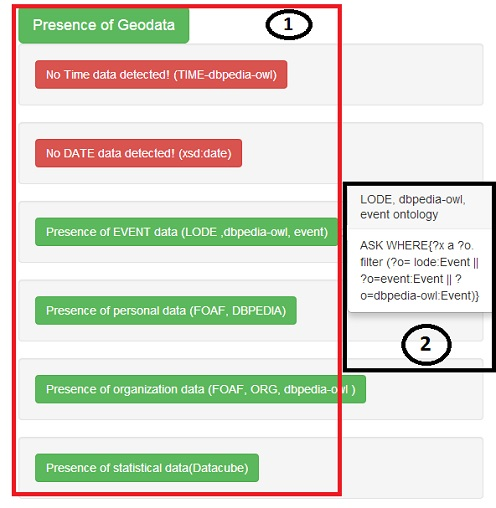
\includegraphics[width=0.4 \textwidth]{img/checkerCategory.png}
}
\subfigure[Overview of the report on categories detected. ]{
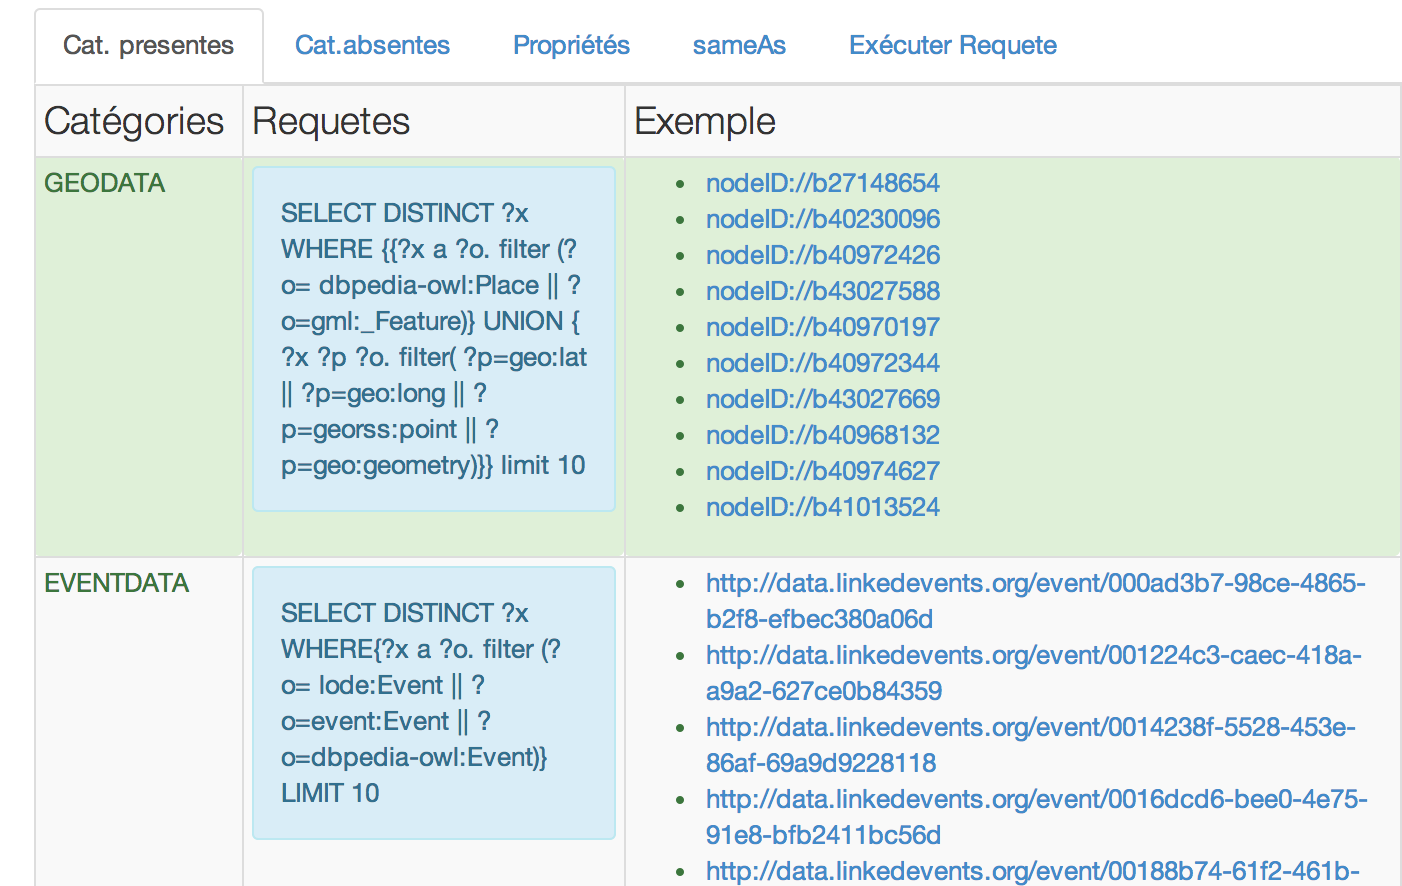
\includegraphics[width=0.4 \textwidth]{img/categories.png}
}
\subfigure[Two views generated by the LD wizard, for geodata and stats data]{
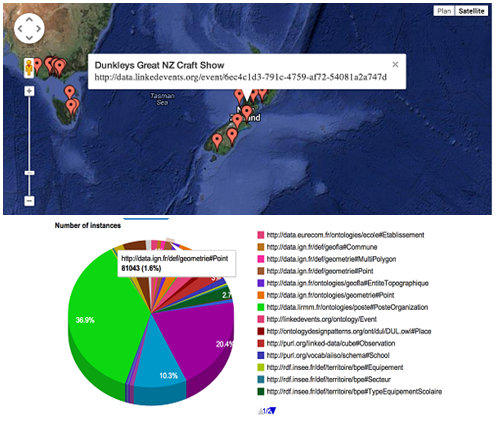
\includegraphics[ width=0.4 \textwidth]{img/samplevisu.png}
}


\caption{Categories detected and visualization generated by the Linked Data visualization wizard in the case of EventMedia endpoint service.}
\label{fig:visuSample}
\end{center}
\end{figure*}

\todo{Review Fig.6.2 b) } \\

\todo{add this work - in discussion http://oai.cwi.nl/oai/asset/13425/13425B.pdf, that seems to have some similar ideas, as well as the work on LDVM pipeline}

\subsection{Discussion}
\label{sec:discuss}


\section{A vocabulary for Describing VIsualization Applications} \label{sec:dvia}

We have implemented a vocabulary, DVIA\footnote{\url{http://bit.ly/Vb4L8k}} aims at describing any applications developed to consume datasets in 4-5 stars, using visual tools to showcase the benefits of Linked Data. It reuses four existing vocabularies: Dublin Core terms at \url{http://purl.org/dc/terms/}, dataset catalogue (DCAT) at \url{http://www.w3.org/ns/dcat#}, Dublin Core Metadata Initiative at \url{http://purl.org/dc/dcmitype} and the Organization vocabulary at \url{http://www.w3.org/ns/org#}.  It is composed of three main classes : 

\begin{itemize}
\item \textbf{Application}: This class represents the application or the mashup developed for demo-ing or consuming data in LD fashion. It is subclass of \textbf{dctype:Software}
\item \textbf{Platform}: The platform where to host or use the application, could be on the Web (Firefox, Chrome, IE, etc..) or mobile (android, iOS, mobile ) or even desktop
\item \textbf{VisualTool}: Represents the tool or library used to build the application. 
\end{itemize}

The diagram of the main classes and properties is depicted in Figure \ref{visuGraphModel}. The current version of the vocabulary in Turtle format can be found at \url{http://purl.org/ontology/dvia} .  Listing \ref{snapshot} is a snapshot of the description of the application which won the Semantic Web Challenge\footnote{\url{http://challenge.semanticweb.org/2012/winners.html}} in 2012, the \textit{EventMedia Live} application, described using DVIA vocabulary. It depicts apart from some metadata about the application (dct:title, dct:name, dct:issued, dct:creator and dct:license), the different visualization libraries integrated for building Eventedia Live (e.g.: Google API, Backbone, etc), as well as the operating systems where it is designed for, the different views/facets available in the application (map, charts, graphs, force-directed layout, ect) and the heteregeneous datasets used to implement it. 

\lstset{basicstyle=\scriptsize, backgroundcolor=\color{white}, frame=shadowbox, caption= {Snapshot in Turtle of the description of Event Media Live Application}, label=snapshot, captionpos=b}
\begin{lstlisting}
visuapp:eventMedia01
       a dvia:Application ; 
       dct:title "EventMedia Live"@en;   
       dvia:description "An application for reconciling Live events with media" ; 
       dvia:url <http://eventmedia.eurecom.fr> ; 
       dct:issued "2012-11-10"^^xsd:date ; 
       dvia:businessValue "not commercial" ;   
       dvia:keyword "events, media"^^xsd:string ; 
       dct:license <http://www.opendatacommons.org/licenses/pddl/1.0/> ; 
      dvia:platform [ a dvia:Platform ; 
			dct:title: "Desktop" ;
			dvia:preferredNavigator "Google Chrome" ; 
			dvia:alternativeNavigator "FireFox" ;
			dvia:system "Mac OS, Windows, Linux"^^string ] ; 
		
     dvia:usesTool [ a dvia:visualTool; dct:title "Google visualization Tool" ; 
	dct:description "Google visualization API" ; 
	dvia:accessUrl <https://developers.google.com/chart/interactive/docs/reference> ; 
	dvia:downloadUrl <http://www.google.com/uds/modules/gviz/gviz-api.js/> ] ;
    dvia:usesTool visuapp:visualTool02 ;
    dvia:consumes [ a dcat:Dataset; dct:title "BBC dump"] ; 
    dvia:consumes [ a dcat:Dataset; dct:title "last.fm scrapped dataset"] ;
    dvia:consumes [ a dcat:Dataset; dct:title "upcoming scrapped dataset"] ;
    dvia:consumes [ a dcat:Dataset; dct:title "eventful scrapped dataset"] ;
    dvia:consumes [ a dcat:Dataset; dct:title "Flickr scrapped dataset"] ;
    dvia:consumes [ a dcat:Dataset; dct:title "Music Brainz "] ;
    dvia:consumes [ a dcat:Dataset; dct:title "Foursquare Json file"] ;
    dvia:consumes [ a dcat:Dataset; dct:title "DBpedia"] ;
    dct:creator [foaf:mbox "khrouf@eurecom.fr"; foaf:name "Houda Khrouf"];
    dct:creator [foaf:mbox "vuk@eurecom.fr"; foaf:name "Vuk Milicik"];
    dct:creator [foaf:mbox "raphael.troncy@eurecom.fr"; foaf:name "Raphael Troncy"];
    dvia:view "map, chart, graph, force-directed layout" ; 
       .
	   ...
	
\end{lstlisting}

The full version of this sample description is available at \url{http://www.eurecom.fr/~atemezin/datalift/visumodel/eventMedia-sample.ttl}. The actual version of the DVIA intends to be small enough to cover the concepts that are needed to reuse partial or full parts of applications. 

\begin{figure}[!htbp]
\vspace{-2.5cm}
  \centering{
    %\leavevmode
      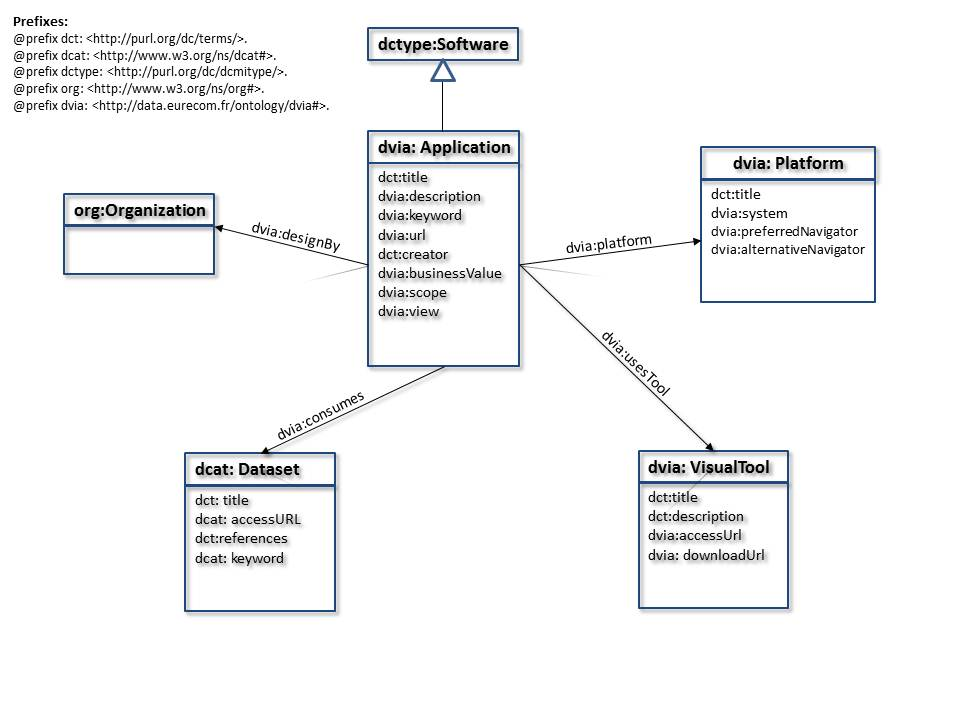
\includegraphics[ height=5in]{img/visuGraphModel.jpg}
  
    \caption{Conceptual Model of the DVIA vocabulary }
    \label{visuGraphModel}
  }
\end{figure}



\subsection*{Summary} \label{sec:conclusion}
% deploy the vocab and setting up a hub for mashups
% find patterns for applications
% develop a recommender for creating applications according to some criteria
\todo{Rewrite properly this section}
\textcolor{red}{We have presented in this paper an approach that could help reusing tools and libraries in the domain of applications built on top of datasets in Linked Open Data. We first presented our motivation as to demonstrate to the end users or decision makers, there is always a need to develop a showcase, hence sometimes looking for analogous or similar applications in the area to ease the process of creation the mashup. We proceeded by surveying some applications to extract relevant common facts worth reusable, from which we proposed a small vocabulary (DVIA)  to semantically describe visual applications. }

\textcolor{red}{We need to validate the DVIA by scrapping and reconciling data from all innovative applications websites and exposed them in RDF, starting with some of those we studied and others applications submitted at the Semantic Web Challenge the past three years. We strongly believe that having such a a hub  describing the tools, datasets, etc.  used to build  applications consuming 4-5 stars datasets will contribute to interoperable Applications leading to a Linked Open Visualizations (LOVIZ) on the LOD cloud.}

\section{Map visualization of Geodata Endpoints}
\label{sec:geordfviz}

With the growing interest of publishing geolocation data according to linked data principles, many endpoints are provided without any visual interface to help navigating on top of the data. This lead to make it difficult for lay users to grab the essence of the data without learning some SPARQL queries. On the other hand, visual depiction of a location in a map makes it easier to identifier a resource. In this work, we present a lightweight tool that help understanding the geodata resources behind any endpoint in a more attractive way to non-experts users. GeoRDFviz is built using generic queries and three visual actions: (i) zooming, (ii) filtering and (iii) describing of resources with geometry.

\begin{figure*}[!htbp]
\begin{center}
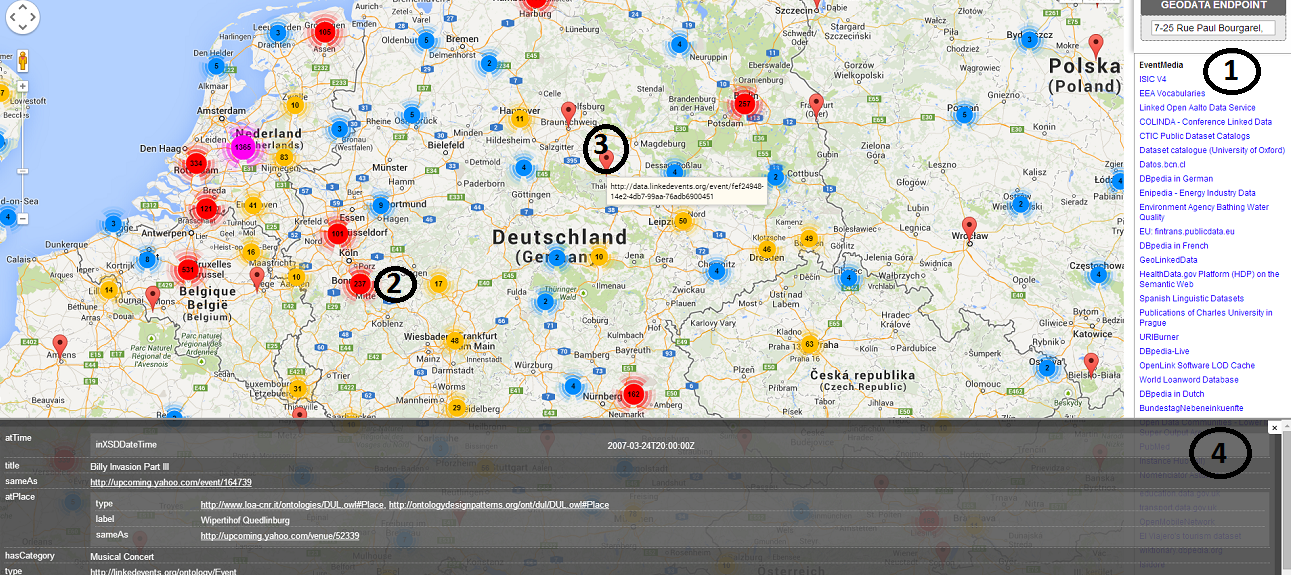
\includegraphics[ width=0.9 \textwidth]{geoRDFvizpic_1200x.png}
\caption{Screenshot of the user interface. The circles with numbers highlight the different elements : (1) list of endpoints, (2) number of resources available in the map area, (3) A zoom to a given element and (4) description of the selected resource.}
\label{fig:geoviz-ui}
\end{center}
\end{figure*}


\subsection{GeoRDFviz System Overview}
\label{sec:system}
\todo{DEscribe here the system}
GeoRDFviz prototype at \url{http://semantics.eurecom.fr/datalift/GeoRDFviz/}

\paragraph{Technology Stack}

\paragraph{Features}




\section{Important Properties for an Entity}
\label{sec:propEntities}
In many knowledge bases, entities are described with numerous properties. However, not all properties have the same importance. Some properties are considered as keys for performing instance matching tasks while other properties are generally chosen for quickly providing a summary of the key facts attached to an entity. Our motivation is to provide a method enabling to select what properties should be used when depicting the summary of an entity, for example in a multimedia question answering system such as QakisMedia\footnote{\url{http://qakis.org/}} or in a second screen application providing more information about a particular TV program\footnote{\url{http://www.linkedtv.eu/demos/linkednews/}}. Our approach consists in: (i) reverse engineering the Google Knowledge Panel by extracting the properties that Google considers as sufficiently important to show (Section~\ref{sec:knowledge-graph}), and (ii) analyzing users' preferences by conducting a user survey and comparing the results (Section~\ref{sec:evaluation}). We finally show how we can explicitly represent this knowledge of preferred properties to attach to an entity using the Fresnel vocabulary~\cite{pietriga2006}. \\
\todo{TODO: ADD reference here?} \\
\todo{ADD figure of GKP search + result of crawling in JSON or implementation code}

\subsection{Reverse Engineering the Google KG Panel}
\label{sec:knowledge-graph}
Web scraping is a technique for extracting data from Web pages. We aim at capturing the properties depicted in the Google Knowledge Panel (GKP) that are injected in search result pages~\cite{Bergman2012}. We have developed a Node.js application that queries all DBpedia concepts that have at least one instance which is \texttt{owl:sameAs} with a Freebase resource in order to increase the probability that the search engine result page (SERP) for this resource will contain a GKP. We assume in our experiments that the properties displayed for an entity are type and context dependent (country, time, query) which can affect the results. Moreover, we filter out generic concepts by excluding those who are direct subclasses of \texttt{owl:Thing} since they will trigger ambiguous queries. We obtained a list of $352$ concepts\footnote{See also the SPARQL query at \url{http://goo.gl/EYuGm1}}.

\begin{algorithm}[h]
\scriptsize
\caption{Google Knowledge Panel reverse engineering algorithm} \label{algoscrapping}
\begin{algorithmic}[1]
    \STATE INITIALIZE $equivalentClasses(DBpedia,Freebase) $ AS $vectorClasses$
    \STATE Upload $vectorClasses$ for querying processing
    \STATE Set $n$ AS number-of-instances-to-query
    \FOR {each $conceptType \in vectorClasses$}
	\STATE SELECT $n$ instances
	\STATE $listInstances \leftarrow$ SELECT-SPARQL($conceptType$, $n$)
		\FOR {each $instance \in listInstances$}
			\STATE CALL http://www.google.com/search?q=$instance$
			\IF {$knowledgePanel$ exists}
				\STATE SCRAP GOOGLE KNOWLEDGE PANEL
			\ELSE
				\STATE CALL http://www.google.com/search?q=$instance + conceptType$
 				\STATE SCRAP GOOGLE KNOWLEDGE PANEL
			\ENDIF
			\STATE $gkpProperties \leftarrow$ GetData(DOM, EXIST(GKP))
			
		\ENDFOR
	\STATE COMPUTE occurrences for each $prop \in gkpProperties$
    \ENDFOR
    \STATE RETURN $gkpProperties$
\end{algorithmic}

\end{algorithm}


For each of these concepts, we retrieve $n$ instances (in our experiment, $n$ was equal to 100 random instances). For each of these instances, we issue a search query to Google containing the instance label. Google does not serve the GKP for all user agents and we had to mimic a browser behavior by setting the $User-Agent$ to a particular browser. We use CSS selectors to check the existence of and to extract data from a GKP. An example of a query selector is $.\_om$ (all elements with class name $\_om$) which returns the property DOM element(s) for the concept described in the GKP. From our experiments, we found out that we do not always get a GKP in a SERP. If this happens, we try to disambiguate the instance by issuing a new query with the concept type attached. However, if no GKP was found again, we capture that for manual inspection later on. Listing~\ref{algoscrapping} gives the high level algorithm for extracting the GKP. The full implementation can be found at \url{https://github.com/ahmadassaf/KBE}. We finally observe that this experiment is only valid for the English Google.com search results since GKP varies according to top level names.


\subsection{Evaluation}
\label{sec:evaluation}
We conducted a user survey in order to compare what users think should be the important properties to display for a particular entity and what the GKP shows.

\subsubsection{User survey.}
\label{sec:survey}
We set up a survey\footnote{The survey is at \url{http://eSurv.org?u=entityviz}} on February 25th, 2014 and for three weeks in order to collect the preferences of users in term of the properties they would like to be shown for a particular entity. We select only one representative entity for nine classes: \texttt{TennisPlayer}, \texttt{Museum}, \texttt{Politician}, \texttt{Company}, \texttt{Country}, \texttt{City}, \texttt{Film}, \texttt{SoccerClub} and \texttt{Book}. 152 participants have provided answers, 72\% from academia, 20\% coming from the industry and 8\% having not declared their affiliation. 94\% of the respondents have heard about the Semantic Web while 35\% were not familiar with specific visualization tools. The detailed results\footnote{\url{https://github.com/ahmadassaf/KBE/blob/master/results/agreement-gkp-users.xls}} show the ranking of the top properties for each entity. We only keep the properties having received at least 10\% votes for comparing with the properties depicted in a KGP. We observe that users do not seem to be interested in the \texttt{INSEE code} identifying a French city while they expect to see the \texttt{population} or the \texttt{points of interest} of this city.

\subsubsection{Comparison with the Knowledge Graphs.}
\label{sec:comparison}
The results of the Google Knowledge Panel (GKP) extraction\footnote{\url{https://github.com/ahmadassaf/KBE/blob/master/results/survey.json}} clearly show a long tail distribution of the properties depicted by Google, with a top N properties (N being 4, 5 or 6 depending on the entity) counting for 98\% of the properties shown for this type. We compare those properties with the ones revealed by the user study. Table~\ref{tab:agreement} shows the agreement between the users and the choices made by Google in the GKP for the 9 classes. The highest agreement concerns the type \texttt{Museum} (66.97\%) while the lowest one is for the \texttt{TennisPlayer} (20\%) concept. We think properties for museums or books are more stable than for types such as person/agent which vary significantly. We acknowledge the fact that more than one instance should be tested in order to draw meaningful conclusion regarding what are the important properties for a type.

\begin{table}[!htp]
\centering{\scriptsize
\begin{tabular}{lccccccccc}
\hline
 \textbf{Classes}	& TennisPlayer 	& Museum & Politician & Company & Country & City & Film & SoccerClub & Book	 \\ \hline
 \textbf{Agr.}& 20\%  & 66.97\% & 50\% & 40\% & 60\% & 60\% & 60\% & 50\% & 60\% \\ \hline
\end{tabular}
\caption{Agreement on properties between users and the Knowledge Graph Panel}
\label{tab:agreement}
}
\end{table}\normalsize

With this set of 9 concepts, we are covering $301,189$ DBpedia entities that have an existence in Freebase, and for each of them, we can now empirically define the most important properties when there is an agreement between one of the biggest knowledge base (Google) and users preferences.

\subsubsection{Modeling the preferred properties with Fresnel.}
\label{sec:fresnel}
Fresnel\footnote{\url{http://www.w3.org/2005/04/fresnel-info/}} is a presentation vocabulary for displaying RDF data. It specifies \textit{what} information contained in an RDF graph should be presented with the core concept \texttt{fresnel:Lens}. We use the Fresnel and PROV-O ontologies\footnote{\url{http://www.w3.org/TR/prov-o/}} to explicitly represent what properties should be depicted when displaying an entity. This dataset can now be re-used as a configuration for any consuming application.

\lstset{basicstyle=\scriptsize, backgroundcolor=\color{white}, frame=single, caption={Excerpt of a Fresnel lens in Turtle}, label=fresnel, captionpos=b}
\begin{lstlisting}
:tennisPlayerGKPDefaultLens rdf:type fresnel:Lens ;
  fresnel:purpose fresnel:defaultLens ;
  fresnel:classLensDomain dbpedia-owl:TennisPlayer ;
  fresnel:group :tennisPlayerGroup ;
  fresnel:showProperties (dbpedia-owl:abstract dbpedia-owl:birthDate
    dbpedia-owl:birthPlace dbpprop:height dbpprop:weight
    dbpprop:turnedpro dbpprop:siblings) ;
  prov:wasDerivedFrom
    <http://www.google.com/insidesearch/features/search/knowledge.html> .	
\end{lstlisting}
\normalsize

\section{Application consuming Event datasets: Confomaton}
\label{sec:confomaton}

In this Section, we aim at creating a rich environment to enable users to navigate events as well as their various representative media such as photos, slides and tweets. A typical usage is to gather data about a scientific conference and investigate the added value of collecting scientific related media. A non trivial task in such application is to connect structured data with extremely noisy content, especially in the case of a major conference.

 We consider a scientific conference, the International Semantic Web Conference (ISWC 2011), which took place in Bonn, Germany last November. Broadly speaking, considering all co-authors, people who have participated in the reviewing process, people who have physically attended the conference or tried to follow it on social networks, we estimate that it has attracted more than 1,500 participants. The conference organizers publish a lot of structured data regarding the conference including the list of accepted papers, their authors and institutions, the detailed program composed of sub-events with the exact timetable and the location (rooms) of the talks. This data is modeled using the SWC ontology\footnote{\url{http://data.semanticweb.org/ns/swc/ontology}}, which is designed to describe academic events, and uses classes and properties from other ontologies such as FOAF (for people) and SWRC (BibTeX elements for the papers). The main conference of type \texttt{swc:ConferenceEvent} is related to a set of sub-events, namely (\texttt{WorkshopEvent}, \texttt{TutorialEvent}, \texttt{SessionEvent}, \texttt{TalkEvent}) via the property \texttt{swc:isSuperEventOf}. Table~\ref{tab:dataset-stats} shows some statistics about the data provided by the Dog Food server regarding the ISWC 2011 conference. We first notice that the data is incomplete. The conference has hosted 16 workshops in total, but the 75 papers are only associated to 8 of them while the 8 others did not have any papers according to the corpus. Furthermore, we find 133 papers that are not connected to any of the events via the predicate \texttt{swc:hasRelatedDocument}. Finally, some useful information is also missing such as the keynote speakers and the \emph{Semantic Web Death Match} (panel) event. This lack of knowledge is also a motivation for our work: can we collect and analyse social network activities in order to complete the factual description of this event?

\begin{table}[htbp]
\footnotesize{
\begin{center}
\begin{tabular}{|r|r|r|r|r|r|}
\hline
\multicolumn{1}{|c}{\textbf{Main Event}} & \multicolumn{1}{|c}{\textbf{Sub-event}} & \multicolumn{1}{|c}{\textbf{Number of events}} & \multicolumn{1}{|c}{\textbf{Papers}} & \multicolumn{1}{|c|}{\textbf{Authors}}\\
\hline
& \texttt{Workshop Event} & 16 & 75 & 185\\
& \texttt{Tutorial Event} & 7 & 7 & 20\\
\texttt{Conference Event} & \texttt{Session Event} & 1 & 66 & 202\\
& \texttt{Talk Event} & 93 & 93 & 275\\
& - & - & 133 & 385\\
\hline
\texttt{Total (distinct)} & 4 & 117  & 292 & 735 \\
\hline
\end{tabular}
\vspace{1mm}
\caption{Metadata provided by the Dog Food Server for the ISWC 2011 conference.}
\label{tab:dataset-stats}
\end{center}}
\end{table}


We collected social network data in real time during the six days of the conference using the main tags advertised by the organizers (\texttt{\#iswc2011}, \texttt{\#cold2011}, \texttt{\#derive2011}, etc.). Table~\ref{tab:media-statistics} shows some statistics about the different media services used by the attendees along with the number of items from a number of distinct users. As expected, Twitter is by far the most used service: we have been able to collect 3,390 tweets from 519 different users. A significant proportion of tweets contains hyperlinks that we have further analysed. Hence, we extracted 384 different websites indexed by so-called URL shorteners (such as Bitly) found in 1,464 tweets (43\% of tweets). These links represent a rich source of media, as they pointed to various Web resources categories such as blogs, slides, photos, publications and projects. For example, 25\% of these links pointed to PDF documents that are generally one of the conference papers but could also be related papers relevant for the followers of the conference. We also analyse these links to extract the various media services used by Twitter.

\begin{table}[htbp]
\centering{
\begin{tabular}{|ll|r|r|}
\hline
\multicolumn{2}{|c}{\textbf{Media Service}} & \multicolumn{1}{|c}{\textbf{Items}} & \multicolumn{1}{|c|}{\textbf{Users}}\\
\hline
\multicolumn{2}{|l|}{Twitter} & 3390 tweets & 519\\
& \hspace{1em}pic.twitter & 12 photos &  6 \\
& \hspace{1em}yfrog  & 10 photos & 9 \\
\multicolumn{2}{|l|}{Twitpic} & 10 photos &  6 \\
\multicolumn{2}{|l|}{Flickr} & 47 photos & 6\\
\multicolumn{2}{|l|}{Google+} & 30 posts & 26\\
\multicolumn{2}{|l|}{Slideshare} & 25 slides & 20 \\
\hline
\end{tabular}
\vspace{1mm}
\caption{Media services used during ISWC 2011 conference}
\label{tab:media-statistics}
}
\end{table}

The name \emph{Confomaton} is a word play on the French term \emph{Photomaton} (English photo booth) and \emph{conference}. Just like a Photomaton illustrates the scene inside of the photo booth, the \emph{Confomaton} illustrates an event such as a conference enriched with social media. \emph{Confomaton} is a Semantic Web application that produces and consumes Linked Data and is composed of four main components (Figure~\ref{fig:architecture}): (i) an Event Collector that extracts events descriptions such as the ones available in the Semantic Web Dog Food corpus; (ii) a media collector that collects social media content and represents it in RDF using various vocabularies; (iii) a Reconciliation Module playing the role of associating social media with sub-events and external knowledge; (iv) a User Interface powered by an instance of the Linked Data API as a logical layer connecting all the data in the triple store with the front-end visualizations.

\begin{figure*}[t!h]
 \centering
 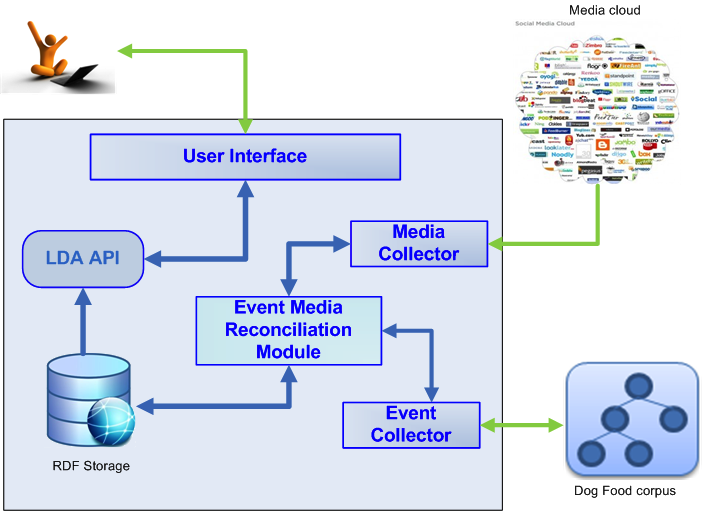
\includegraphics[scale=0.35]{img/architecture.png}
 \caption{\emph{Confomaton} general architecture.}
 \label{fig:architecture}
\end{figure*}


%%%  3.1 Media Collector  %%%
\subsection{Media Collector}                                                \label{sec:media-collector}
In the context of \emph{Confomaton}, we have developed so-called \emph{media collectors} with the purpose of searching various social networks and media platforms for event-related media items such as photos, videos, and slides. We currently support 4 social networks (Google+, MySpace, Facebook, and Twitter) and 7 media platforms (Instagram, YouTube, Flickr, MobyPicture, img.ly, yfrog and Twitpic). Our approach being agnostic of media providers, we offer a common alignment schema for all of them:
\begin{itemize}
  \item	\textbf{Media URI}, the deep link to the media item, e.g. \url{http://farm7.staticflickr.com/6059/6290784192_567346ba6a_o.jpg}
  \item \textbf{Type}, the type of the media item, e.g.  ``photo''
  \item \textbf{Story URI}, the URI of the micropost or story where the media item appeared, e.g. \url{http://www.flickr.com/photos/96628098@N00/6290784192/}
  \item \textbf{Message}, the concrete micropost or description text in raw format, e.g.  ``Laura. \texttt{\#iswc2011}, \texttt{\#semanticweb}, \texttt{\#bonn}, \texttt{\#germany}''
  \item \textbf{Clean}, the concrete cleaned micropost or description text with some characters (e.g. hash signs) removed, e.g. ``Laura. iswc2011, semanticweb, bonn, germany''
  \item \textbf{User}, the URI of the author of the micropost, e.g. \url{http://www.flickr.com/photos/96628098@N00/}
  \item \textbf{Published}, the timestamp of when the micropost was authored, or the media item was uploaded, e.g. \texttt{2011-10-27T12:24:41Z}
\end{itemize}

\begin{lstlisting}[caption={Sample output of the media collector showing Google+ and Flickr results using \#iswc2011 as query term},label={lst:media}]
{
  "GooglePlus": [
    {
	  "mediaurl": "http://software.ac.uk/sites/default/files/images/content/Bonn.jpg",
	  "storyurl": "https://plus.google.com/107504842282779733854/posts/6ucw1Udb5NT",
	  "message": {...}
    }],
    "Flickr": [
   {
      "mediaurl": "http://farm7.staticflickr.com/6226/6290782640_e8a1ffdcc2_o.jpg",
      "storyurl": "http://www.flickr.com/photos/96628098@N00/6290782640/",
      "message": {..}
    }]
 }
\end{lstlisting}

In order to retrieve data from media providers, we use the particular media provider's search Application Programming Interfaces (API) where they are available, and fall back to Web scraping the media provider's website if not. In some cases, we initially use the search API, but then have to fall back to Web scraping in order to get more details on the results, such as the \textbf{Media URI}, which is not exposed by all APIs. From all media providers, Twitter plays a special role, as it can serve as a host for other media providers. For example, it is very common for tweets to contain links to media items hosted on external media providers such as Twitpic. Other media providers treat media items as first class objects, i.e. have dedicated object keys in their API results for media items, which is not in all cases true for Twitter. We handle this by searching for a list of URIs of known media providers in combination with the actual search term. To illustrate this, when searching for media items for the search term ``ISWC 2012'' on Twitter, we would actually search for ``iswc 2012 AND (twitpic.com OR flic.kr)'' in the background, whereas on all other media providers, the search term ``iswc 2012'' is sufficient. The media collector can be tested at \url{http://webmasterapp.net/social/}.

\subsection{Data Modeling}
We have developed an Event Collector, which takes as input the Dog Food corpus described using the SWC ontology and converts all events into the LODE ontology\footnote{\url{http://linkedevents.org/ontology/}}, a minimal model that encapsulates the most useful properties for describing events. We use the Room ontology\footnote{\url{http://vocab.deri.ie/rooms}} for describing the various rooms contained in the conference centre. An explicit relationship between an event and its representative media (photo, slide, micropost, etc.) is realised through the \texttt{lode:illustrate} property. For describing those media, we re-use two popular vocabularies: the W3C Ontology for Media Resources\footnote{\url{http://www.w3.org/TR/mediaont-10/}} for photos and videos, and SIOC\footnote{\url{http://rdfs.org/sioc/spec/}} for tweets, status, posts and slides. The example below shows how a tweet is represented in \emph{Confomaton}.
{\footnotesize 	
\begin{verbatim}
<http://data.linkedevents.org/tweet/af557cef-5d5b-49c6-a4c3-bc9c41ce1555>
 a sioc:Post;
 dcterms:created "2011-10-23T13:34:03+00:00";
 sioc:content    "@smeh Good luck for your presentation at #ssn2011...";
 sioc:hasCreator <http://www.twitter.com/BadmotorF>;
 lode:illustrate <http://data.semanticweb.org/workshop/ssn/2011>;
 gc:hashtag      "#ssn2011";
 owl:sameAs      <http://twitter.com/BadmotorF/status/128071685235671040>.
\end{verbatim}
}

Figure~\ref{fig:natasha-example} depicts how all these vocabularies are used together. The ISWC 2011 conference is illustrated by a photo shared on Flickr, has for sub-event the EvoDyn 2011 workshop in which one of the tweets posted mentioned the recognised named entity Nathasha Noy who is also a general chair of the conference. All the data is available in the \emph{Confomaton} graph in a public SPARQL endpoint available at \url{http://semantics.eurecom.fr/sparql}.
\begin{figure*}[t!h]
 \centering
 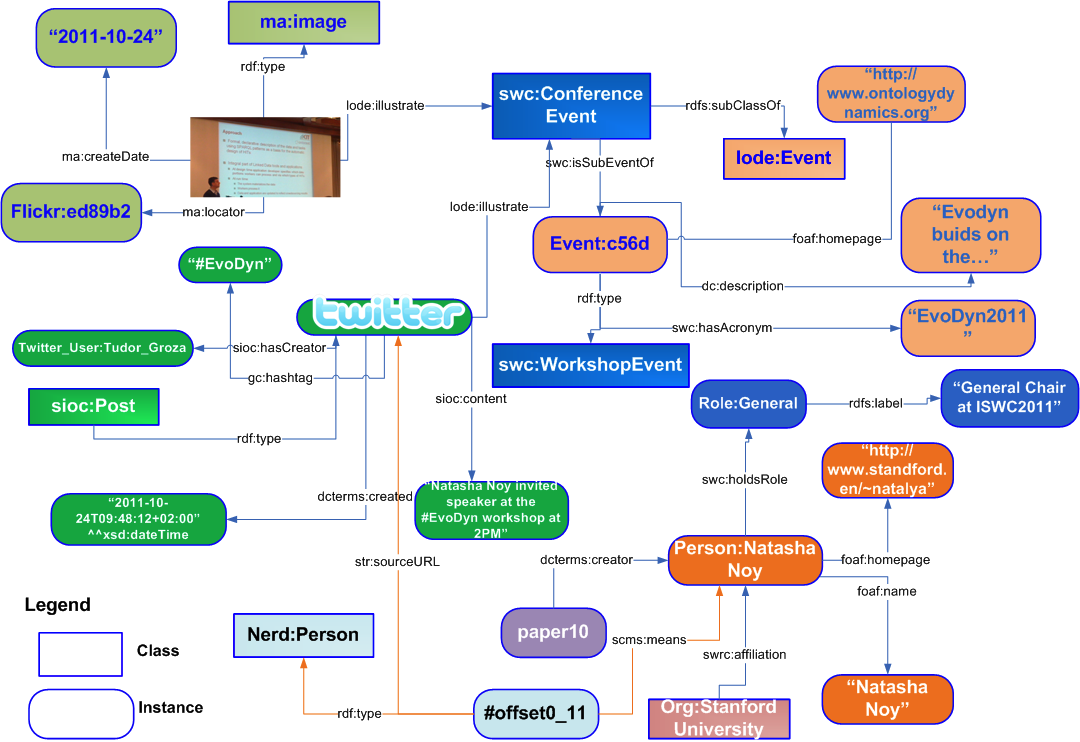
\includegraphics[scale=0.3]{img/natasha_example.png}
 \caption{Example of data modeled in \emph{Confomaton} re-using multiple vocabularies}
 \label{fig:natasha-example}
\end{figure*}



\subsection{Event Media Reconciliation Module}
The event media reconciliation module aims to align the incoming stream of social media with their appropriate events and to interlink some descriptions with general knowledge available in the LOD cloud\footnote{\url{http://lod-cloud.net/}} (e.g. people and institutions descriptions). Attaching social media to fine-grained events is a challenging problem. We tackle it by pre-processing the data with two successive filters in order to reduce the noise: one of them relies on keyword search applied to some fields such as title and tag, while the other one filters data based on temporal clues. The reconciliation is then ensured through a pre-configured mapping between a set of keywords and their associated events. This map enables us to associate media with the macro-events that people explicitly refer to in their posts or photos. For example, we connect all media items containing the tag \texttt{\#iswc2011} with the general ISWC 2011 conference. However, this method is absolutely not convenient to associate media items with sub-events. For instance, in the ISWC 2011 conference, there are 99 sub-events of type \texttt{TalkEvent}, which could be the presentation of a paper, a keynote speech or any other kind of talk. Social network users typically do not specify a particular tag for such events. We hence advocate the need for more advanced classifiers to associate media with sub-events. These classifiers can exploit a variety of parameters such as social network graphs and named entities extracted from media content. 

\subsection{Graphical User Interface}
The Graphical User Interface (GUI) of \emph{Confomaton} is built around four perspectives characterising an event: (i) \textit{``Where does the event take place?''}, (ii) \textit{``What is the event about?''}, (iii) \textit{``When does the event take place?''}, and finally (iv) \textit{``Who are the attendees of the event?''}. In addition, the user interface offers full text search for these four dimensions. The \emph{Confomaton} user interface is powered by the Linked Data API\footnote{\url{http://code.google.com/p/linked-data-api/wiki/Specification}}, which provides a configurable way to access RDF data using simple RESTful URLs that are translated into queries to our SPARQL endpoint. More precisely, we use the Elda\footnote{\url{http://code.google.com/p/elda}} implementation developed by Epimorphics. Elda comes with some pre-built samples and documentation, which allow to build specification to leverage the connection between the back-end (data in the triple store) and the front-end (visualizations for the user). The API layer helps to associate URIs with processing logic that extract data from the SPARQL endpoint using one or more SPARQL queries and then serialize the results using the format requested by the client. A URI is used to identify a single resource whose properties are to be retrieved or to identify a set of resources, either through structure of the URI, or through query parameters.

\autoref{lst:config} shows an example of the configuration file of the \emph{Confomaton} API specifying the event, media and tweet viewers followed by the events and media properties access.
\begin{lstlisting}[caption={Example configuration file of the \emph{Confomaton} API, specifying event properties access.},label={lst:config}]
<#MyAPI> a api:API ;
	rdfs:label "Confomaton API"@en ;
	api:endpoint <#event>,<#media>,<#tweet>,<#agent>, <#venue>,<#user>,<#eventbyid>,<#mediabyid>,<#tweetbyid>,<#agentbyid>,<#venuebyid>,<#userbyid>;
	api:sparqlEndpoint <http://semantics.eurecom.fr/sparql> ;
# specification of the event viewer (all properties appear in the json file)
spec:eventViewer a api:Viewer ;
  api:property "title","description","space.lat","space.lon","time.datetime","inagent.label",...
<#eventbyid> a api:ItemEndpoint;
		api:uriTemplate "/event/{id}";
		api:itemTemplate "http://data.linkedevents.org/event/{id}";
		api:defaultViewer spec:eventViewer.		
\end{lstlisting}

The system is available at \url{http://semantics.eurecom.fr/confomaton/iswc2011}. On the left side of the main view, the user can select the main conference event or one of the sub-events as provided by the Dog Food metadata corpus. In the centre, the default view is a map centred on where the event took place (e.g. Bonn, Germany) and the user is also encouraged to explore potential other types of events (concerts, exhibitions, sports, etc.) happening nearby, this data being provided by EventMedia~\cite{Troncy:ISEMANTICS10}. The \textit{What} tab is media-centred and allows to quickly see what illustrates a selected event (tweets, photos, slides). Zooming in an event triggers a popup window that contains the title and timetable of the event, the precise room location and a slideshow gallery of all the media items collected for this event. For the \textit{When} tab, a timeline is provided in order to filter events according to a day time period. Finally, the \textit{Who} tab aims at showing all the participants of the conference. This is intrinsically bound to a social component, aiming not only to present relevant information about participants (their affiliations, homepages, or roles at the conference), but also the relationships between participants themselves and with events.


\section{Application consuming Statistics datasets: PerfectSchool}
\label{sec:perfectSchool}

\subsection{Scope of the Application}
The \texttt{Perfect School} application is intended to provide useful information on schools in France using semantic technologies, with RDF-ized data enriched with other datasets in the wild. The application and the vocabulary have successfully passed the integrity checker\footnote{\url{http://www.w3.org/2011/gld/wiki/Data_Cube_Implementations}}  of an implementation for the candidate recommendation of Data Cube \url{http://www.w3.org/TR/vocab-data-cube/ } vocabulary at W3C.

\subsection{Legacy Datasets}
In order to build the application, we had to look at some relevant datasets in data.gouv.fr. The ones selected for building the application are the following:

\begin{itemize}
\item The file at \url{http://www.data.gouv.fr/DataSet/564055} in CSV format, containing a list of $67, 201$ schools (name, status, type), with geolocation position in Lambert 93, for the academic year 2011-2012. The file contains the following attributes (in French): 
	\begin{itemize}
		\item code of the school (e.g. 0010002X), 
		\item  official name of the school (e.g.: College Saint-Exupery), 
		\item principal name (e.g. COLLEGE), 
		\item patronymic name (e.g. Saint-Exupery), 
		\item status of the school (1 = open, 2 = to be closed and 3 = to be opened), 
		\item label of the type of school (e.g: 1= first degree, 3 = second degree).
	\end{itemize}
\item \url{http://www.data.gouv.fr/DataSet/572165}, in .CSV format giving results for professional schools, indicators), from one academic year (2011-2012). The file contains the following attributes:
	\begin{itemize}
		\item name of school, 
		\item  city code, 
		\item code of the school, 
		\item district where the school is located, 
		\item sector (PR= PRivate, PU= PUblic), 
		\item several observation measures with statistics on success rates, school versus academic/national rates, name of the academy it belongs to, as well as the department.
	\end{itemize}
   \item \url{http://www.data.gouv.fr/DataSet/572162} (.CSV) containing statistics for  $2296$ public high schools and indicators. It complements the statistics from INSEE.
\end{itemize}

\subsection{Ontology Modeling}
We have reused some external ontologies for more interoperability:
\begin{itemize}
\item \texttt{aiiso}\footnote{http://vocab.org/aiiso/schema} for the type of school and codes of school.
\item \texttt{geofla}\footnote{http://data.ign.fr/def/geofla\#} since the schools are considered as a topographic entities,
\item \texttt{geom}\footnote{http://data.ign.fr/def/geometrie\#} for representing the different geometries (points with latitude and longitude) in a given coordinate reference systems with \texttt{ignf} ontology at \url{http://data.ign.fr/def/ignf#} . 
\item \texttt{skos:Concept} for describing the 30 types of nature of schools. 
\item \texttt{qb:DimensionProperty}\footnote{http://www.w3.org/TR/vocab-data-cube/} and \texttt{qb:MeasureProperty} for modeling the dimensions and different indicators available for a given school. 
\end{itemize}
The resulting vocabulary is available at \url{http://purl.org/ontology/dvia/ecole}. 

We use the Datalift platform for transforming the different CSV files into RDF. The final data is available  at \url{http://eventmedia.eurecom.fr/sparql} with the named graph \texttt{http://data.eurecom.fr/school}.

\subsection{URI Policies}
We use the following patterns for the URIs of the vocabularies or the resources in our namespace.
\begin{itemize}
\item URI for vocabulary: \texttt{http://data.eurecom.fr/ontologies/\{SECTOR\}}. \\
e.g: \url{<http://data.eurecom.fr/ontologies/ecole>} for the ontology that we have developed.

\item URI for resources: \texttt{http://data.eurecom.fr/id/\{SECTOR\}/\{CLASS\}}. \\
e.g: \url{<http://data.eurecom.fr/id/school/>} for the schools URIs, \\
\url{<http://data.eurecom.fr/id/school/slice/>} for \texttt{qb:Slice}s.

\item URI for taxonomies: we use \texttt{SKOS} for modeling concepts and codes as the following: \\
\texttt{http://data.eurecom.fr/codes/\{SECTOR\}/\{CONCEPT-TYPE\}/\{CODE\}}. 
e.g.: \url{<http://data.eurecom.fr/codes/ecole/natureUAI>} for the collection of natures of the schools ; \\
        \url{<http://data.eurecom.fr/codes/ecole/natureUAI/101>} for a particular concept with code \textit{101} and label '''\'{E}cole maternelle".

\end{itemize}

Besides the aforementioned policy, each school in the user interface can be reached on the UI by using directly the following URI: 
 \url{http://semantics.eurecom.fr/datalift/PerfectSchool/#school/{SCHOOL-CODE/}}, with \{SCHOOL-CODE/\} in lowercase. 
 
\paragraph{\textit{Example:}}
\textit{The school ``Albert Camus'' in the city ''Le Mans'' with the code school $0720800D$ can we viewed in the application directly at} \url{http://semantics.eurecom.fr/datalift/PerfectSchool/#school/0720800d/}

\subsection{Sample School Data in RDF }

\lstset{basicstyle=\scriptsize, backgroundcolor=\color{white}, frame=single, caption= {Snapshot in Turtle for the school ID=0750676C, also at \url{http://semantics.eurecom.fr/datalift/PerfectSchool/\#school/0750676c/}}, label=snapshot, captionpos=b}
\begin{lstlisting}

school:0750676c 	a	aiiso:School,  geofla:EntiteTopographique .
school:0750676c 	a	ecole:Etablissement .
school:0750676c	rdfs:label	"LYCEE DORIAN (PROFESSIONNEL)"@fr ;
school:0750676c	dcterms:title	"Lycee polyvalent et lycee des metiers de la .."@fr ;
	aiiso:code	"0750676C" ;
	ecole:denominationPrincipale "LPO LYCEE DES METIERS"@fr ;
	ecole:patronyme	"DORIAN"@fr ;
	ecole:ville	"PARIS 11"@fr ;
	ecole:codeCommune	"75111" ;
	ecole:secteur	"PU" ;
	ecole:academie	"PARIS"@fr ;
	ecole:departement	"PARIS"@fr ;
	ecole:cycle	"3"^^xsd:int ;
	ecole:etat	"1"^^xsd:int ;
	ecole:nature	bpenat:306 .

slice:0750676c	ecole:etablissement	school:0750676c .
school:0750676c	geom:geometrie	_:vb42480647 , _:vb42531960 .		 

_:vb42480647 a geom:Point;
	geom:systCoord ignfr:wgs84g;
	geom:coordX "48.85429801"^^xsd:double;
	geom:coordY "2.39231163"^^xsd:double . 

_:vb42531960 a  geom:Point;
	geom:systCoord ignfr:ntflamb2e ;
	geom:coordX "655410.1"^^xsd:double;
	geom:coordY "6861755.9"^^xsd:double .
     
	
\end{lstlisting}

\subsection{Interconnection}
For the interconnection process, we didn't use the current module. Instead of that we have used the Silk \cite{jentzsch2010silk} platform as it is re-packaged in the workflow of Datalift. We believe the scripts used for this task can be easily reused within the Datalift platform. Two datasets where used for finding \texttt{owl:sameAs} links:
\begin{enumerate}
\item DBpedia French chapter\footnote{\url{http://fr.dbpedia.org/sparql}}, as the scope of the application was limited to France. We have found only 7 match links with our schools datasets.
\item LinkedGeoData\footnote{\url{http://linkedgeodata.org/sparql}}, as the underlying data used comes from the community project Open Street Map (OSM). Here, we got  a total of $601$ matching links in the category of \texttt{lgdo:BuildingSchool}\footnote{\url{http://linkedgeodata.org/ontology/BuildingSchool}}. 
\end{enumerate}

\subsection{User Interface}
The target device for the application is Mobile phone, using principally two frameworks: Jquery mobile\footnote{http://jquerymobile.com/} and  backbone javascript\footnote{\url{http://backbonejs.org/}}. 
The application provides geolocation, search by city/district, graph charts for stats, table views of relevant results aggregated or group by some other aspects. 
\texttt{Perfect School Application} provides 3 main views:
\begin{enumerate}
\item \textbf{Search form:} The interface retrieves the location automatically ( \'{a} la Google Maps API fashion) , and offers box choices based on the School type: First degree / second degree. When choosing first degree, the user can further select one of (primary school, elementary school or other). For the second degree, apart from looking for one of College, high school or other, the user can look for public or private schools. The search button launches the query behind the scene for retrieving the collection of data matching the user's criteria. 

\item \textbf{Results of searching}: The search action returns a collection of schools plotted in a map. A cursor on the left side helps users zoom to get more details about schools retrieved in a given region, or street. When selecting a given school, the name is displayed and with the possibility to see the route from the barycenter of the result on the map.
\item \textbf{Description of the school:} It is divided in 3 different tabs: (a) General information (name, cycle, principal denomination, nature and patronym used) ; (b) Stats with all the different statistics in form of charts, graphs comparing the school with the others ; and (c) DBpedia-FR\footnote{\url{http://fr.dbpedia.org}} information if available, obtained with the \texttt{owl:sameAs} links for enriching the original dataset with  information such as founder, date of creation, web site, population, head of school etc.

\end{enumerate}

The Figure ~\ref{fig:searchingSchool} shows the three different views on a running example.


\begin{figure*}[!htbp]
\begin{center}
\subfigure[Search options]{
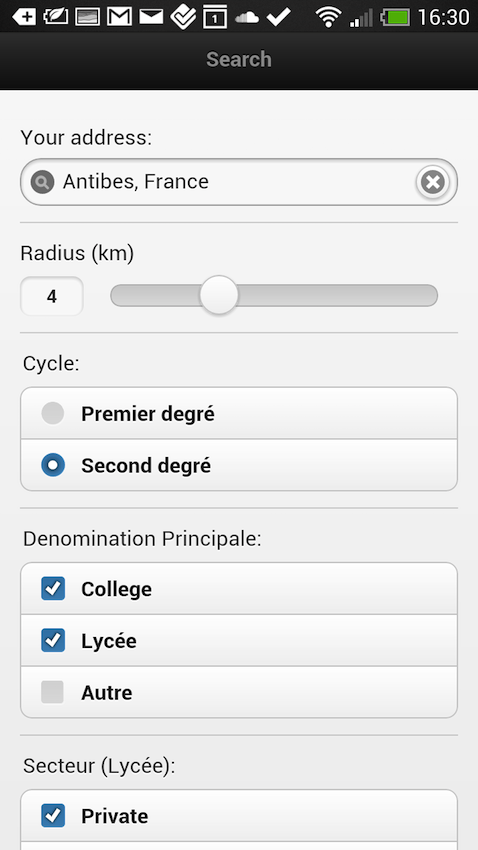
\includegraphics[height=62mm,width=42mm]{img/searching.png}
}
\subfigure[Results displaying on a map]{
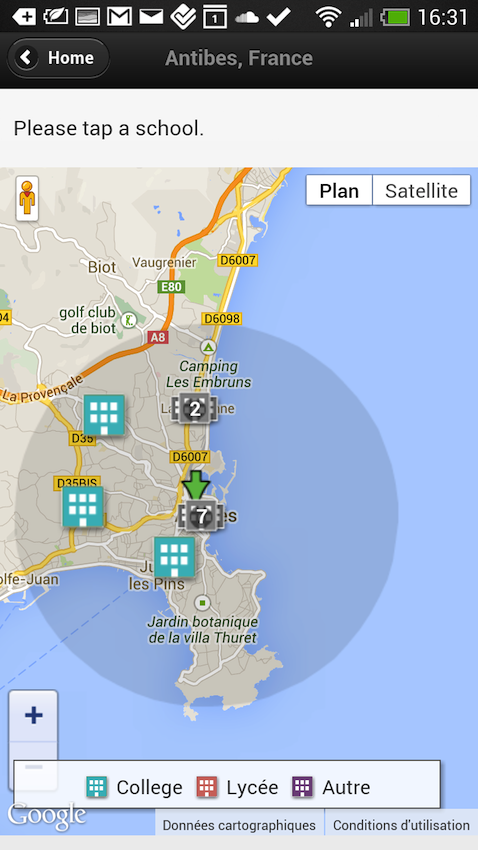
\includegraphics[height=62mm,width=42mm]{img/result.png}
}
\subfigure[Route to the selected school]{
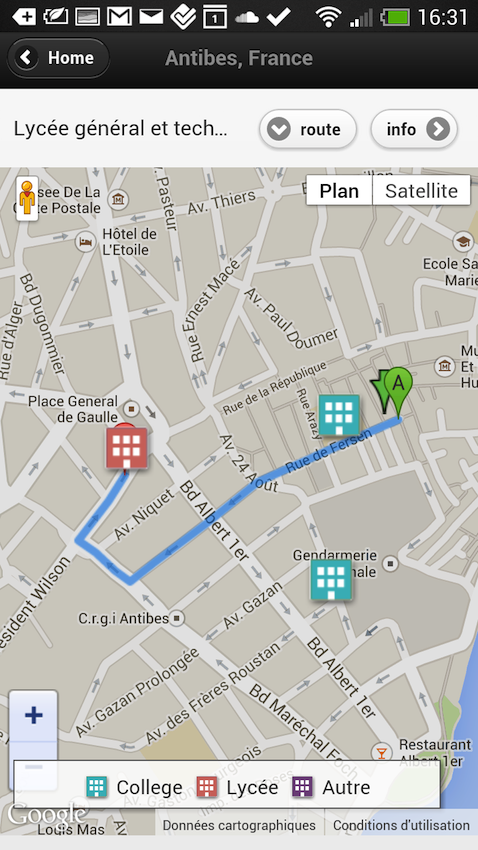
\includegraphics[height=62mm,width=42mm]{img/routeresult.png}
}
\subfigure[Details information with 3 tabs: General, statistics and DBpedia]{
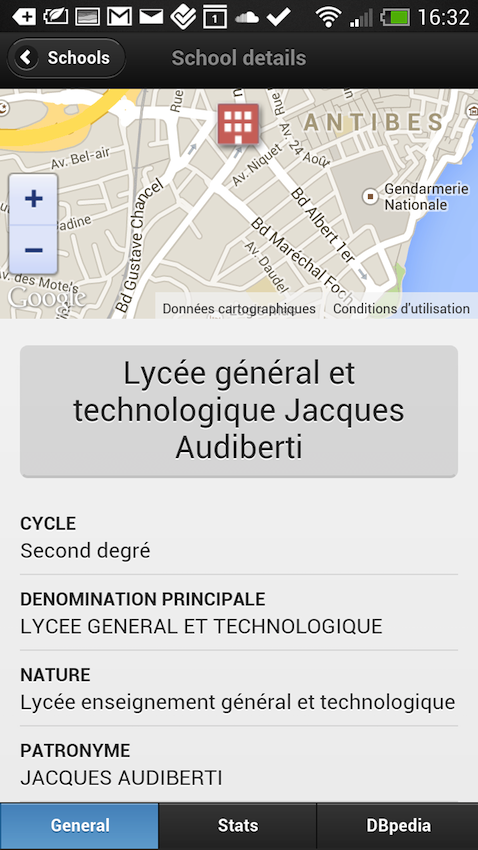
\includegraphics[height=62mm,width=42mm]{img/tab-result.png}
}
\caption{Steps for searching high schools in Antibes in a radius of 4000m, France}
\label{fig:searchingSchool}
\end{center}
\end{figure*}



\section{Improving the discovery of applications contests in Open Data Events}
\label{sec:contests}

\todo{add Alexis work + add appendix of content scrapping and JS apps installation }

\subsection{Background}
\label{sec:backcontest}
One of the challenges in the Apps for Europe -project - and open data projects in general - is the discovery of existing applications using the open data. The discovery of existing applications and ideas is important in order to prevent people from reinventing the wheel, when they instead should put their effort in refining existing applications or developing completely new applications. This will hopefully lead to more diverse applications and furthermore also to higher quality applications, because the existing applications can be enhanced by other people and organizations \cite{apps4eu}. 

In order to promote the reuse and discovery of open data applications, Apps for Europe has created an RDF vocabulary\footnote{\url{https://github.com/mmlab/apps4eu-vocabulary}}  that can be used for describing open data events and also the applications that have been built on top of the open data. Furthermore, Apps for Europe has also developed a Wordpress plugin\footnote{\url{https://github.com/mmlab/AppsForX }}  that open data event organizers can install on their web pages, to make it simpler to populate the RDF data for the events and applications.


\subsection{Modeling events and applications in RDF}
\label{sec:modeleventsapps}

One of the key factors in improving the discovery of open data events is to present the information in a structured machine readable format, so that applications (such as crawlers) can easily consume the data. This follows the Semantic Web movement, where the goal is to convert the current, unstructured documents (readable by humans) into structured documents.

In order to present the event and application information in structured format, Apps for Europe has created an RDF vocabulary available a \url{https://github.com/mmlab/apps4eu-vocabulary/} for modeling the events and applications. The quality of this vocabulary was tested by manually modeling past events  and applications and looking for potential problems and improvements in the ontology. The problems and improvements made to the ontology is presented below.

\begin{figure}[!htbp]

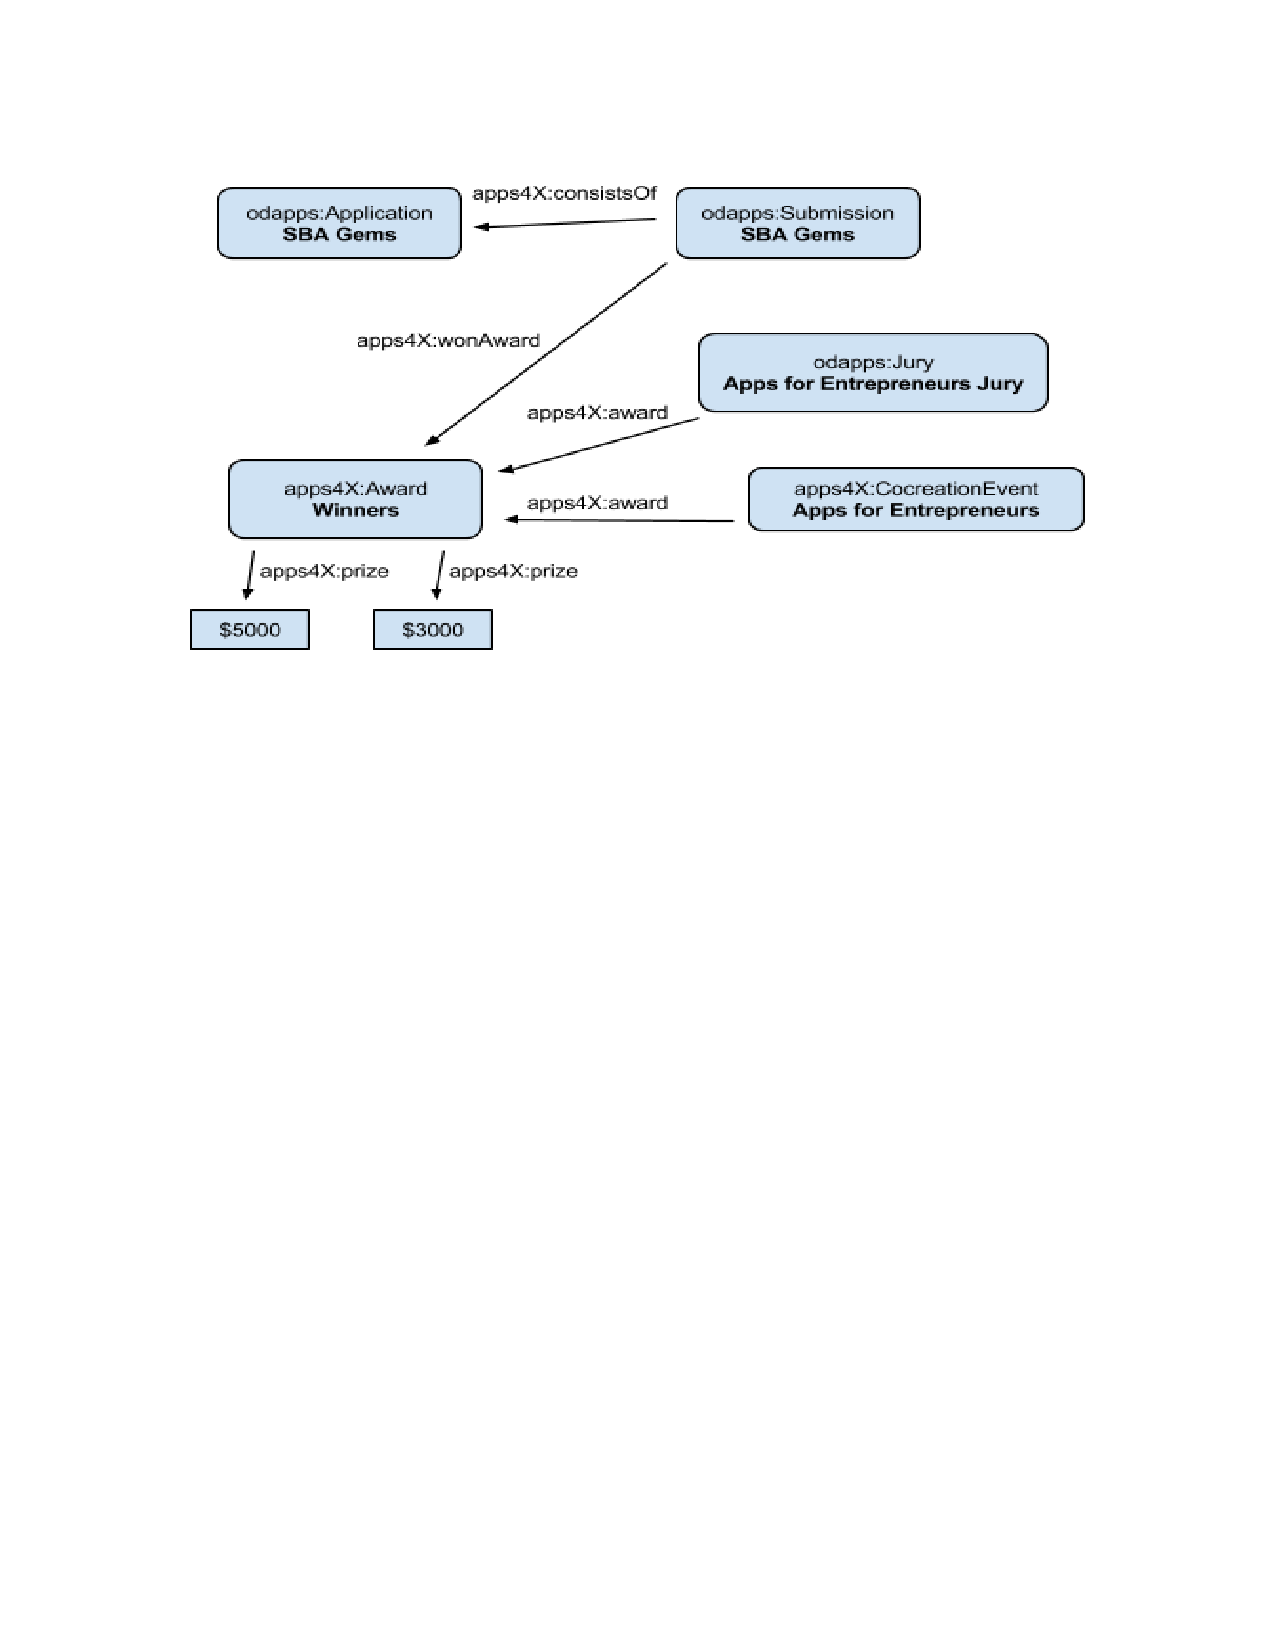
\includegraphics[]{img/rdfTriplesBeforeChanges.pdf}
\caption{The RDF triples before changes. Here we state that the application SBA Gems has won an award in the event Apps for Entrepreneurs. }
\label{fig:modelA}
\end{figure}

In \ref{fig:modelA}, the model is complex, because it requires us to specify an extra class (\texttt{:Submission}) in order to use the \texttt{:wonAward-property}, and yet we are unable to specify which prize the application won (\$5000 or \$3000). While in ~\ref{fig:modelB}, the model is straightforward to specify that an application (SBA Gems) won a prize, because we don't need to use the Submission intermediate class. We are also able to specify which prize the application won (\texttt{:FirstPrize}). It should be notice  also that now the jury is connected to a prize by specifying a jury-attribute for prizes (instead of having a prize-attribute for the jury i.e. direction of the arrow changed).

\begin{figure}[!htbp]
\centering{
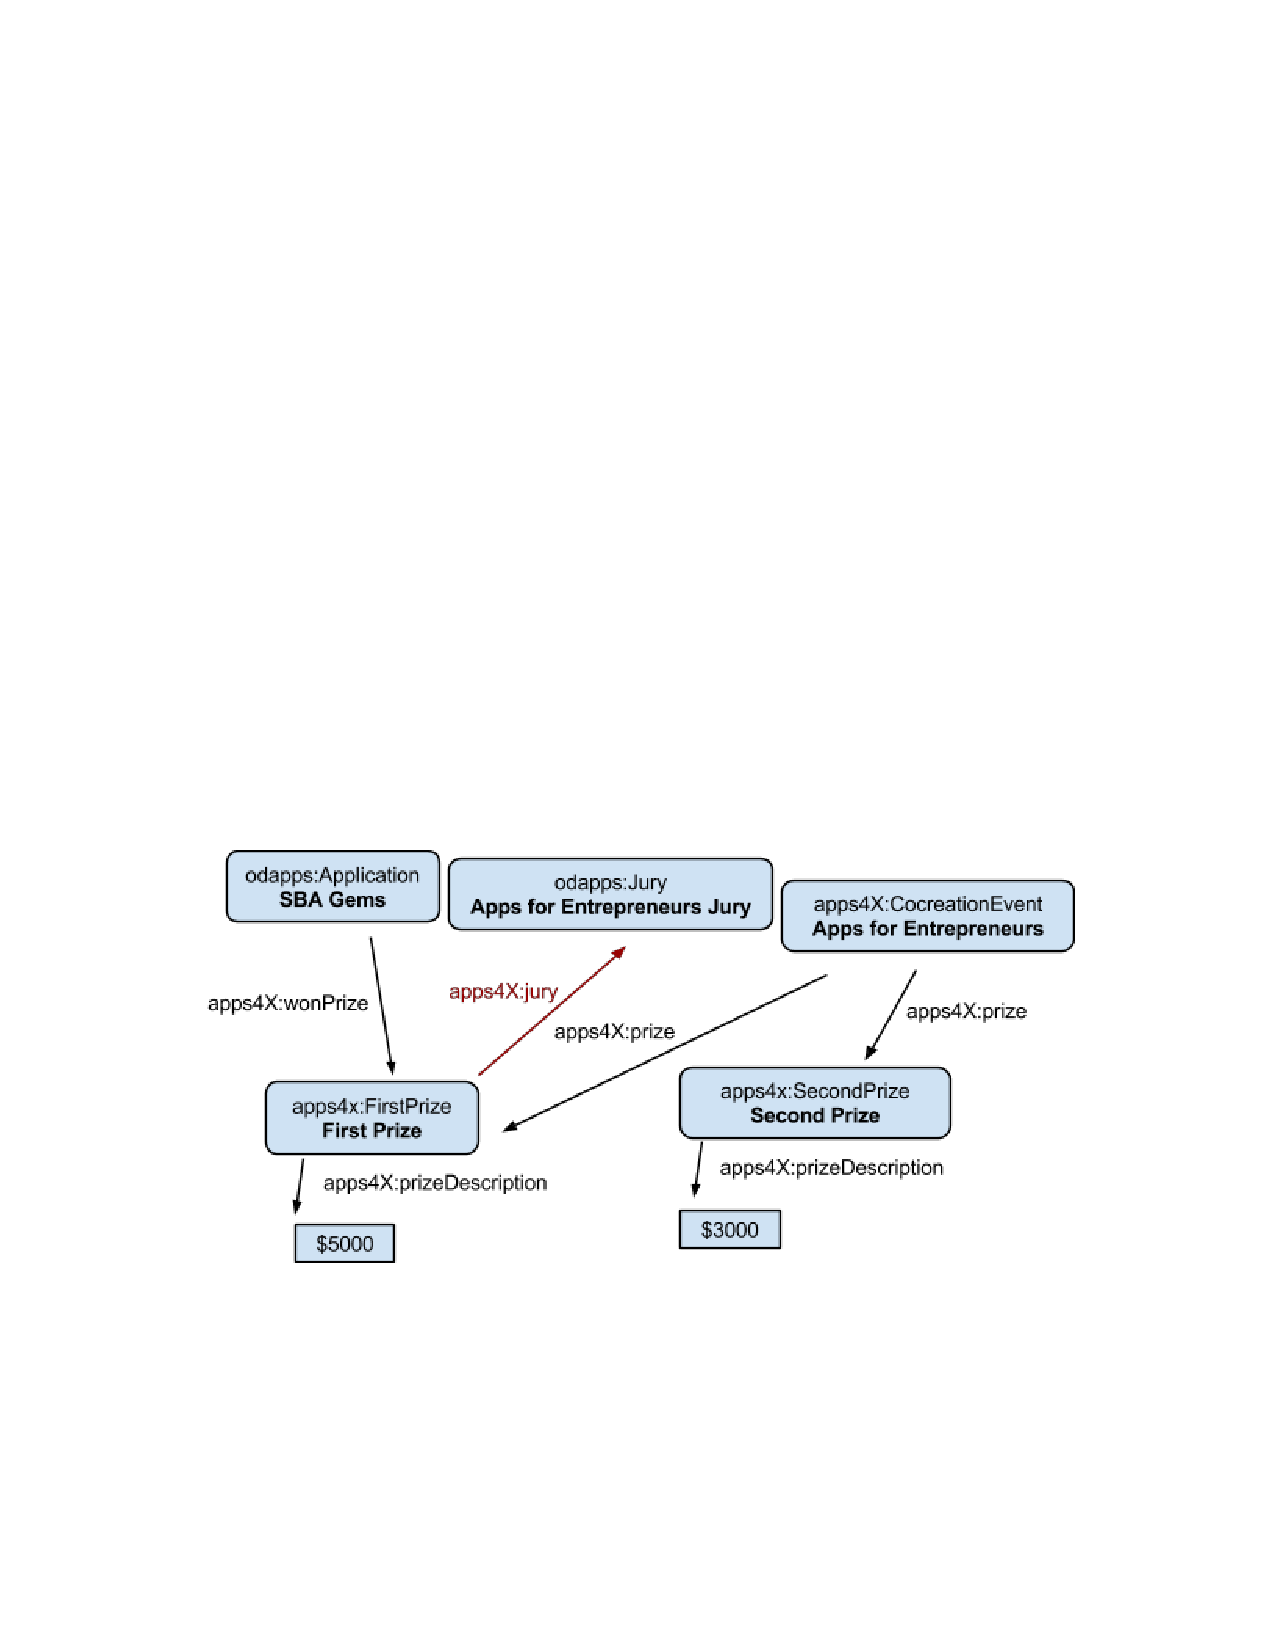
\includegraphics[]{img/rdfTriplesAfterChanges.pdf}
\caption{The RDF triples after changes.}
\label{fig:modelB}
}
\end{figure}

\subsection{Improving the model for specifying winners}
Open data events often include competitions where the best applications are rewarded, and this information was modeled in the Apps for Europe RDF vocabulary as well. However, we found that the current model for this was unnecessarily complicated and therefore the model was simplified. Previously, winning apps required a separate ``Submission''-class in order to state that they had won a competition. Furthermore, the vocabulary didn't allow to state which position (winner, second, third etc.) the winning application was awarded. These problems were fixed by introducing a new property ``wonPrize'' for applications, so that we can directly state that an application won a prize without needing to have an intermediary ``Submission''-class, and by introducing the new classes ``FirstPrize'', ``SecondPrize'', and ``ThirdPrize'' that are all subclasses of the ``Prize''-class. We concluded that it is satisfactory to be able to state positions one to three for the winning apps, and therefore we didn't implement a more complicated vocabulary that would have enabled to state an arbitrary position (by having a position attribute for the prize for example).

Also some other minor changes were suggested for the vocabulary:
\begin{itemize}
\item Use the word ``Prize'' instead of ``Award'' (i.e. rename in all places)
\item Normalize the values for juryRate and usersRate attributes (because otherwise they can't be compared to each other)
\item alternatively reuse the review vocabulary from vocab.org\footnote{\url{http://vocab.org/review/terms.html }}  or schema.org\footnote{\url{http://schema.org/Review}} 
\item Introduce properties \texttt{connectedApp} (for Event) and \texttt{connectedEvent} (for Application), so that applications and events can be linked together.
\end{itemize}


\subsection{Universal JavaScript plugin for RDF population}
\label{sec:plugin}

The inspiration for the JavaScript based solution came from services like \url{https://muut.com/}, which offers embeddable commenting and discussion forums and it can be installed on any web page independent of the CMS. Since almost all people have JavaScript support enabled in their browsers\footnote{ According to a study by Yahoo only about 1\% have JavaScript disabled in their browsers. Source: \url{https://developer.yahoo.com/blogs/ydnfourblog/many-users-javascript-disabled-14121.html} [Referenced 2014-06-02]}  it enables us to implement a solution that can be installed on any web page and also works on almost any browser.

The most striking difference between the CMS based plugin and the JavaScript plugin is the user base, since the JavaScript solution works on any web page while the CMS plugin obviously only can be installed on a dedicated websites. Also the technical approach differs significantly, because in the CMS based approach the server will do all the work for producing the HTML and RDFa markup for the events, while in the JavaScript approach it is the client browser that is responsible for this task.


\paragraph{Technical description}
The JavaScript plugin consists of three distinct parts that are technically independent of each other, but they can still be deployed on the same server if needed:

\begin{enumerate}
\item RESTful  API for creating, editing and removing events and applications from the database.
Both interfaces listed below (2 and 3) communicates and manipulates the data using the RESTful API
\item Admin interface for event organizers
Event organizers manage their events and applications through this interface, which is provided as a ``software as a service'' (SaaS\footnote{\url{http://en.wikipedia.org/wiki/Software_as_a_service}}).
\item Embeddable script that will display the event and application information both in human readable form and in computer readable form (RDFa format) on the event organizers web page.
The script will fetch the event and application information using the RESTful API and then manipulate the document object model (DOM ) after page load and inject the event and application description into the DOM.
\end{enumerate}

The different components are also presented in Figure \ref{fig:jsplugin}

\begin{figure}[!htbp]
\centering{
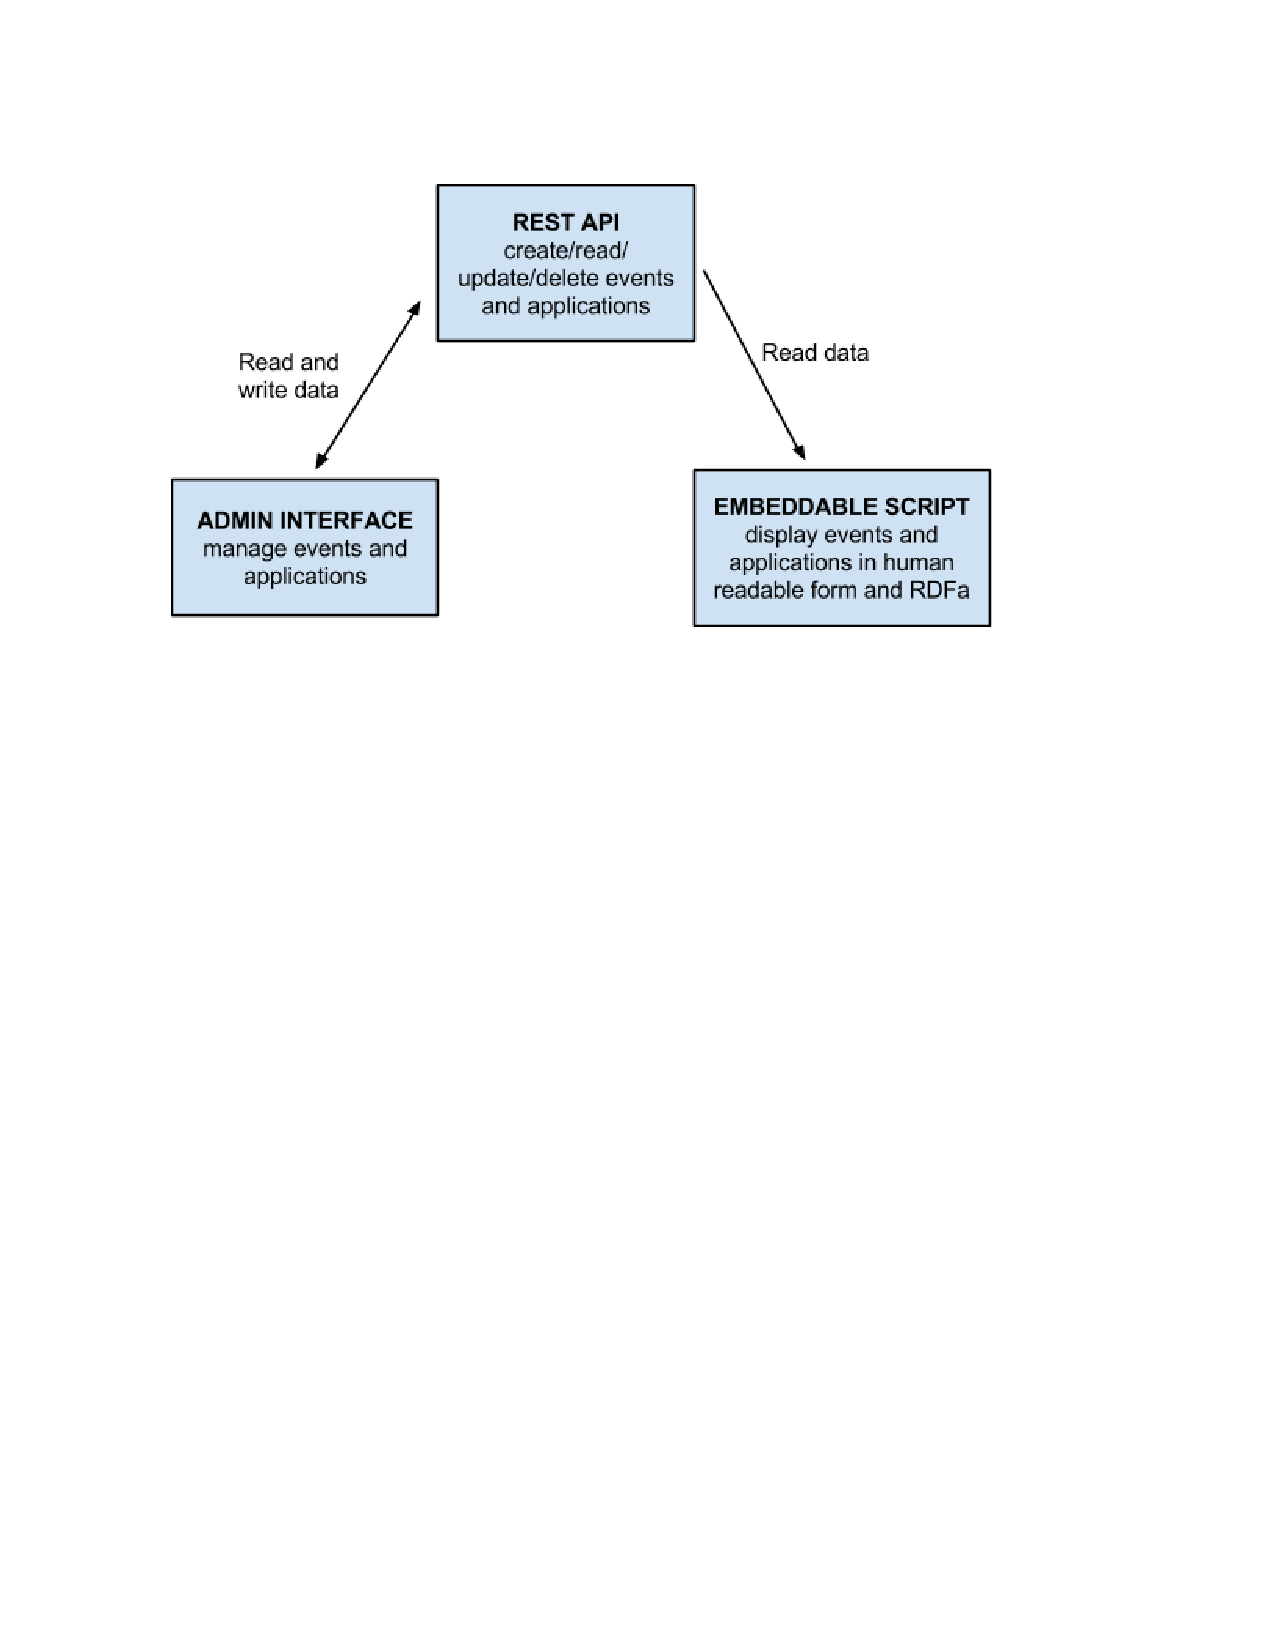
\includegraphics[]{img/componentsJSplugin.pdf}
\caption{Universal JavaScript components}
\label{fig:jsplugin}
}
\end{figure}

The API was implemented in Node.js\footnote{\url{http://nodejs.org/}} , which is a platform for running applications written in JavaScript on server side. It is built on Google Chrome's JavaScript runtime and provides very good performance thanks to it's asynchronous data manipulation model . Node.js has become very popular recently and there is a huge number of third party extensions and frameworks written for it. Furthermore, since the programming language is JavaScript, many libraries and frameworks written for browsers will also function in Node.js. For more details on how to configure the plugin, the readers are encouraged to read the Appendix \ref{ch:appendixA}.

The data is stored in MongoDB, which is the leading NoSQL database\footnote{\url{http://www.mongodb.com/leading-nosql-database}}. In addition to this Mongoose\footnote{\url{http://mongoosejs.com/index.html}} object data mapper  was used in order to simplify the data manipulation and to give structure to the database. Finally, node-restful  was used to transform the Mongoose schema into a working REST API. Node-restful internally relies on Express , which is the most popular web application framework for Node.js.

\paragraph{Admin Interface}
The admin interface provides an intuitive and easy-to-use interface for event organizers to manager their events and the related applications. It is provided as software as a service and will be hosted and managed by Apps for Europe. Event organizers will register to the service and after this they have access to all the features of the admin interface. Two screenshots of the service is presented in Figure \ref{fig:adminInterface} .


The admin interface is implemented in HTML, CSS and JavaScript. Bootstrap\footnote{\url{http://getbootstrap.com/}}  was used as a CSS framework. It simplifies the development of responsive websites and also provides clean aesthetics for the website. AngularJS\footnote{\url{https://angularjs.org/}}  was used as a JavaScript framework.

\begin{figure}[ht!]
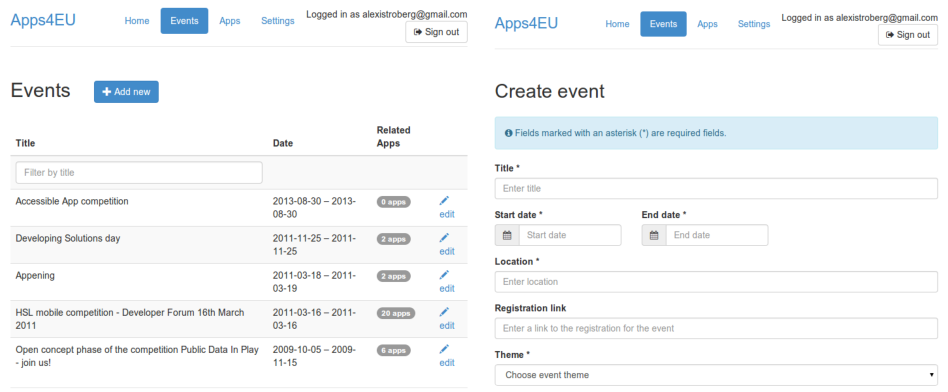
\includegraphics[scale=0.95]{img/adminInterface.pdf}
\caption{Screenshots of the admin interface. On the left is the event listing
 page and on the right is the form for creating an event.}
 \label{fig:adminInterface}
\end{figure}


\paragraph{Embeddable script}
The last component of the puzzle is the embeddable script, that is responsible of displaying the event and application information in human readable form on the event organizer's website. The event organizer will get the embed code from the admin interface, which he will then insert into the HTML code of his website. The embed code is just a reference to an external JavaScript file that will be loaded from the Apps for Europe server and then executed in the browser. A detailed description of how the script works is given below:
\begin{algorithm}
\textsl{
1. The event organizer will embed the code on his own web page.\\
2. On page load, the <script>-tag is parsed by the browser and the actual script is loaded from the Apps for Europe -server.\\
3.	The script is executed.\\
(a).	The script will fetch the event or application information using an AJAX-request.\\
(b).	After the server has responded with the event/application information, the information is displayed on the page in human readable form by modifying the DOM of the page. Furthermore, the same information is presented also in computer readable format by embedding RDFa in the DOM.
}

\end{algorithm}


\subsection{Creating the Knowledge-base for past events}
The final task was to create the knowledge base for past events by using the Apps for Europe RDF vocabulary and generating data to feed the endpoint at \url{http://apps4europe.eurecom.fr/sparql} . The list of events was extracted from the Apps for Europe Google spreadsheet\footnote{\url{https://docs.google.com/spreadsheet/ccc?key=0AiXRLGASq8I0dDlfZURkWGpSODBJaWotQUp3eGNwNGc&usp=sharing}}.

The goal was to populate the events and applications, so that they would follow and fulfill the Apps for Europe vocabulary as well as possible. However, the format and information provided on the event web pages varied, and therefore we were usually only able to populate the following information for most of the events:
\begin{itemize}
\item Title
\item Dates (start and end date)
\item Description (free text)
\item Prizes (if the event included an application contest)
\item Jury members (if the event included an application contest)
\item Location (usually only country was known)
\end{itemize}

Similarly, the information provided for applications varied even more, and sometimes we were able only to populate the title, description and the homepage of the application. Because of these problems, the data populated into the triple store doesn't include all the information we would have hoped to have.

The original idea was to automate the triple store data population as far as possible using content scraping , but because of the heterogeneity of the web pages (in terms of structure and data)  a semi-automated approach was used. Especially the problems listed below prevented a fully automatic approach from being implemented:

\begin{itemize}
\item because of the heterogeneity in the structure of the web pages, it is for example extremely hard to ``automatically'' know which part of the page contains the event location or application homepage link
\item many links to the event pages were broken, and thus manual work was required in order to relocate the actual page
\end{itemize}

In order to be as efficient as possible in the data population the semi-automatic approach was used. Here, the key idea was to populate event pages having only a few application entries (less than 10) manually using the JavaScript plugin, and for the rest of the event pages web scraping was used to populate the application entries (the scraping script had to be configured for each event website separately). \textcolor{red}{The script for this is provided in Appendix B.}

The goal was to populate all the past events (112 in total). However, many of the websites for the past events had already disappeared or didn't include enough information for data population. Furthermore, the data population process turned out to take much more time than anticipated, and therefore we managed to populate only 28 events and in total 889 application entries. The average number of application entries per event was 34 and the median 22.

Visualizations and applications could be built on top of the knowledge base, but because of the small size of the current knowledge base, it is difficult to extract quantitative data from the knowledge base. Some ideas for visualizations are presented below:
\begin{itemize}
\item Map visualization of where past events have been organized
\item Most popular categories/themes for applications
\item Gallery of application screenshots (visual inspiration for developers).
\end{itemize}


The dataset is available below in different formats as dump for download in RDF/Turtle and MongoDB:

\begin{itemize}
\item RDF in turtle format: \url{https://www.dropbox.com/s/3075qsblxzau2fk/rdfInTurtleFormat.tar.gz} 
\item MongoDB dump: \url{https://www.dropbox.com/s/m2sr4na12v3yk07/apps4europe.tar.gz} 
\end{itemize}

\subsection{Discussion}
The embeddable script is non-optimal in the sense that the event or application information is loaded only after the actual page (where the script is embedded) has loaded. This causes some additional delay before the page is fully rendered, but the problem can be alleviated by showing loading indicators.

CSS styling for the events and applications is provided using Bootstrap. All CSS rules have been made specific to the container div-element of the plugin, in order to prevent the CSS from conflicting with the CSS of the page. In the future, another solution called shadow DOM could be used to prevent conflicts between different components of the page, but at the moment the browser support for shadow DOM\footnote{\url{http://caniuse.com/shadowdom}} is not satisfactory. Since the event and application information is directly embedded on the page using DOM, the event organizer can add his own CSS styling to the plugin by overriding the provided CSS rules.

The RDF information about events and applications is populated only if event organizers actually use it on their websites, and therefore it is crucial to ensure that the plugin is appealing in the eyes of the event organizers. It would be especially useful to study the usability of the plugin and also discuss with the event organizers how well the Apps for Europe ontology fits with their data model. In addition to this, also the security of the JavaScript-plugin should be improved, although the information entered to the plugin is not very critical from a security perspective.

\section{Summary}
\label{sec:summarych5}
\todo{extend to reflect all the content of the chapter}

In this chapter we have presented  an approach for creating visualizations on top of Linked Data based on Semantic Web technologies. We first defined seven categories of objects worth viewing in a dataset, and we propose to associate them with commonly used and domain vocabularies. We then present a description of the main components of a Linked Data Visualization Wizard. We describe a lightweight implementation in javascript as a \textit{proof-of-concept} of our proposal, with the benefits to be usable on-line or being extensible. We advocate that such a tool can be easily integrated  in any workflow for publishing and linking data on the web, such as Datalift\ref{SECTION-DATALIFT} or the GeoKnow Stack\ref{SECTION-GEOKNOW}. 

\clearpage

%\chapter*{Part 3 - Contribution to Standards}
\label{part:part3}
 
 \vspace{10mm}
\section*{Summary}
In this part, we present the various work and contributions around the Linked Open Vocabularies ( catalog description, vocabulary publications, APIs and endpoints); prefixes harmonization, vocabulary ranking metrics using information content. We also present some insights on checking licenses compatibility between vocabularies and datasets with the defeasible deontic logic for creating an automatic tool for licenses checking.  We then finish by highlighting our contribution to the GLD WG with the 2 document notes and vocabularies standardized: DCAT, Data Cube, ORG, etc. 
 
%\clearpage
\part{Contribution to Standards}

\chapter{Best Practices for publishing Government Data}
\label{ch:ch6}

\begin{itemize}
\item start from Best practices life-cycle
\item selection/reuse vocabs with LOV by describing LOV
\item harmonize prefixes
\item ranking vocabularies for assessing in catalogs
\end{itemize}

\todo{Find intro life-cycle by Sarven -}
\todo{Start here with the GLD diagram in the publication life-cycle, with emphasis on Datalift one}

\section{Introduction}
What this chapter is about, what we are achieving and introduce the various sections


\section{Catalog of Vocabularies}
\label{sec:catalog}
While we refer the reader to~\cite{AquinJoWS12} for a systematic survey of ontology libraries, we give our own classification of ontology repositories (Table~\ref{tab:catalogs}). In particular, we distinguish six categories of catalogs:
\begin{itemize}
 \item \textit{Catalogs of generic vocabularies/schemas} similar to the LOV catalog, but without any relations among the vocabularies. Example of catalogs falling in this category are vocab.org\footnote{\url{http://vocab.org/}}, ontologi.es\footnote{\url{http://ontologi.es/}}, JoinUp Semantic Assets or the Open Metadata Registry.
 \item \textit{Catalogs of ontologies for a specific domain} such as biomedicine with the BioPortal\footnote{\url{http://bioportal.bioontology.org/}}, geospatial ontologies with SOCoP+OOR\footnote{\url{http://socop.oor.net/}}, Marine Metadata Interoperability and the SWEET ontologies\footnote{\url{http://sweet.jpl.nasa.gov/2.1/}}.
 \item \textit{Catalogs of ontologies from a project} such as the famous DAML repository of ontologies\footnote{\url{http://daml.org/ontologies/}}.
 \item \textit{Catalogs of ontology Design Patterns (ODP)} focused on reusable patterns in ontology engineering.
 \item \textit{Catalogs of editors' ontologies} used to test some features of a tool and to keep track of the ontologies built by a tool, such as Web Prot\'{e}g\'{e} or TONES.
 \item \textit{Catalogs of ontologies maintained by a single organization} which often uses a platform such as Neologism\footnote{\url{http://neologism.deri.ie}} for publishing vocabularies.
 \item \textit{Vocabularies crawled by Semantic Web search engines} containing snapshots at the time of the crawsuch as Watson\footnote{\url{http://watson.kmi.open.ac.uk/}}, Sindice\footnote{\url{http://www.sindice.com}}, Falcon-s\footnote{\url{http://ws.nju.edu.cn/falcons/}} or Swoogle. For example, the NanJing Vocabulary Repository (NJVR)- a dump of Falcon-s ontologies, reported as of June, 17th 2,996 vocabularies crawled from 261 pay-level domains.
\end{itemize}

\begin{landscape}
\begin{table}[!htbp]
\centering{
\begin{tabular*}{15cm}{lcccc}
\specialrule{1pt}{1pt}{1pt}
 Catalog	& Number of  	& Search Feature 	& Category  & Vocabulary	 \\
 name       & vocabularies  &  & & maintenance \\
 \specialrule{1pt}{1pt}{1pt}
 vocab.org 	&19 				& No & Catalog of & N/A		\\
		& 				&      &  generic vocabularies &     \\ \hline
ontologi.es    & 39         &No  & -//-  & N/A \\ \hline
Joinup Semantic & 112 & Yes & -//- & Yes \\
Assets &  & & & \\ \hline
Open Metadata & 308 & Yes & --//-- & Yes \\
Registry  & & & & \\  \hline
BioPortal & 355 & Yes & Catalog of & Yes \\
	    &        &       & Domain vocabularies & \\ \hline
SOCoP + OOR &40 & Yes & --//-- & Yes \\ \hline
Marine Metadata & 55 & Yes & --//--& Yes \\
Interoperability & & & & \\ \hline
SWEEET 2.2 & 200 & No& --//-- & N/A \\ \hline
DAML & 282 & No& --//-- &  No   \\ \hline
ODPs &101 & No& Catalog of ODPs & Yes \\ \hline
vocab.derie.ie & 68 & No & Catalog of & Yes \\
		   & & & Organizations & \\ \hline
data.lirmm.fr & 15 & No & --//- & Yes \\
ontologies & & & & \\  \hline
TONES & 219 & No & Catalog of & N/A \\
           &         &      & editors' vocabularies & \\ \hline	
Web Prot\'{e}g\'{e} & 69 & No & --//-- & Yes \\
\specialrule{1pt}{1pt}{1pt}
\end{tabular*}
\caption{Catalogs of vocabularies with respectively the number of the ontologies, the presence of a search feature, the catalog category and whether it is maintained or not}
\label{tab:catalogs}
}
\end{table}
\end{landscape}

We observe that the existing catalogs of vocabularies in the literature have some limitations compared with LOV. In terms of coverage, the number of vocabularies indexed by LOV is constantly growing and it is the only catalog, to the best of our knowledge, that provide all types of search criteria (metadata search, within/across ontologies search), both an API and a SPARQL endpoint access and that can be as well classified as an ``Application platform'' apart from being at the same time an ontology directory and an ontology registry. According to the categories of ontology libraries defined in~\cite{AquinJoWS12}, LOV falls under the category of ``curated ontology directory'' and an ``application platform'' because the ontologies are curated manually with statistics automatically generated, and because it exposes its data via an API. Furthermore, LOV provides an answer to some of the issues mentioned in the survey reported in~\cite{AquinJoWS12}, such as ``where has an ontology been used before?'' or ``is this ontology compatible with mine?''. In particular, LOV provides vocabulary usage statistics of the LOD Cloud datasets and it exposes vocabularies dependency using the Vocabulary-of-A-Friend (VOAF) ontology.

vocab.cc\footnote{\url{http://vocab.cc}} is a service which is similar to prefix.cc since it enables to look up and search for Linked Data vocabularies while providing more specific information about the usage of a particular class or property in the Billion Triple Challenge Dataset (BTCD). It also provides the ranking of those properties or classes. The authors mentioned that ``common prefixes are resolved with data from prefix.cc''. Although they don't give further details, this service is somehow related to prefix.cc. Triple-Checker\footnote{\url{https://github.com/cgutteridge/TripleChecker}} is a web service based on prefix.cc which aims at finding typos and common errors in RDF data. It parses a given URI/URL and the output is divided in two sections: the namespaces and the term section. The former matches against prefix.cc to determine whether they are ``common prefixes'' and the latter provides the term definition.

\section{Linked Open Vocabulary (LOV) and Vocabularies}        \label{sec:lov-approach}
The Linked Open Vocabularies (LOV) initiative aims to bring more insights about published vocabularies in order to foster their reuse. Compared to other projects, LOV benefits from a community:
\begin{itemize}
 \item to assess the quality (including documentation, metadata) and the reuse potential of a vocabulary before it is indexed. LOV contains currently 350+ reusable and well-documented vocabularies;
 \item to augment vocabularies with explicit information not originally defined in the RDF vocabulary. For example, only 55\% of vocabularies have explicit metadata of at least one creator, contributor or editor. In LOV, we augmented this information leading to more than 85\% of vocabularies with this information;
 \item to automatically extract the implicit relations between vocabularies using the Vocabulary Of Friend\footnote{\url{http://lov.okfn.org/vocab/voaf/}} (VOAF) ontology. These relations can be used as a new metric for ranking terms based on their popularity at the schema level;
 \item to consider vocabulary semantic in the result ranking: a literal value matched for the \texttt{rdfs:label} property has a higher score than for the \texttt{dcterms:comment} property.
\end{itemize}

The way vocabularies are considered in LOV is similar to the way datasets are considered in the LOD cloud~\cite{Bizer2009}. Hence, while the Vocabulary of Interlinked Datasets (VoiD) is used to describe relationships between datasets and their vocabularies~\cite{alexander2009}, VOAF is used to describe the mutual relationships between vocabularies. VOAF itself reuses over popular vocabularies such as Dublin Core Terms (dcterms), Vocabulary Of Interlinked Datasets (VoiD), Vocabulary for ANNotating vocabulary (vann) and the BIBliographic Ontology (bibo). The vocabulary also introduces new classes such as \texttt{voaf:Vocabulary} and \texttt{voaf:VocabularySpace}.

The LOV-Bot is the tool that automatically keeps up-to-date the relationships and the metadata about the vocabularies indexed in LOV, using the following steps:
\begin{itemize}
  \item	LOV-Bot daily checks for vocabularies update (any difference in the vocabulary formal description fetched using content negotiation);
  \item	LOV-Bot uses SPARQL constructs to detect relationships and metadata and creates explicit metadata descriptions in the LOV dataset;
  \item	LOV-Bot annotations are then listed in a back-office administration dashboard in order to be reviewed. This manual part enables LOV curators to interact with vocabularies authors and the wider community to raise issues and make remarks or suggestions.
\end{itemize}
The LOV dataset is synchronized with the information presented in the web site. The latter allows a human user to browse LOV information.  The Linked Open Vocabularies initiative does not only monitor the current state of the ecosystem. It also aims at storing and giving access to vocabularies history. To achieve this goal, the LOV database contains every different version of a vocabulary over the time since its first issue. For each version, a user can access the file and a log of modifications since the previous version.

\subsection{Linked Open Vocabularies}     \label{sec:lov}

Started in March 2011, in the framework of the DataLift research project \cite{scharffe_2012} hosted by the Open Knowledge Foundation, the Linked Open Vocabularies (LOV) initiative is now standing as an innovative observatory of the vocabularies ecosystem. It gathers and makes visible indicators not yet harvested before, such as interconnection between vocabularies, versioning history and maintenance policy, past and current referent (individual or organization) if any. The number of vocabularies indexed by LOV is constantly growing (390 as of January 2014) thanks to a community effort and it is the only catalog, to the best of our knowledge, that provide all types of search criteria (metadata search, within/across ontologies search), both an API and a SPARQL endpoint access. According to the categories of ontology libraries defined in~\cite{AquinJoWS12}, LOV falls under the category of \textit{``curated ontology directory''}  and \textit{``application platform''}. 

The development of LOV has highlighted a number of interesting research issues such as \textit{``where to find the best domain vocabulary to reuse?"}, and \textit{``is it possible to create a curated catalogue of vocabularies that are links?"}
Below we illustrate some of the LOV features useful for ontology search and reuse activities:
  
 \begin{description}
	\item [Domain filtering.] Each vocabulary is inserted into LOV according to its domain and/or scope. This information is guided by the scope of the vocabulary, such as City, Science, Library, Metadata, Media, etc. This feature helps in disambiguating the results of the querying service and to classify vocabularies. 
	\item [Content aware Search.] If the searched term matches a \url{rdfs:label} it will have a higher score than if it matches \url{dcterms:comment}.
	\item [Links between vocabularies.] One of the key feature of LOV design is the explicit links between vocabularies, 
	 \item [Scope of LOV.]The intended use is to promote and facilitate the reuse of vocabularies in the linked data ecosystem.
	 \item [Vocabulary Curation.]The collection of the vocabularies is maintained by curators in charge of validating and inserting vocabularies in the LOV ecosystem, by taking care of the versions of the vocabulary and giving some reviews. The vocabulary is then automatically enriched with more information about the datasets using it, and relations to other vocabularies.
 \end{description}

\todo{reference the image of vocabs evolution in LOV}

\begin{figure}[h!t]
\centering
  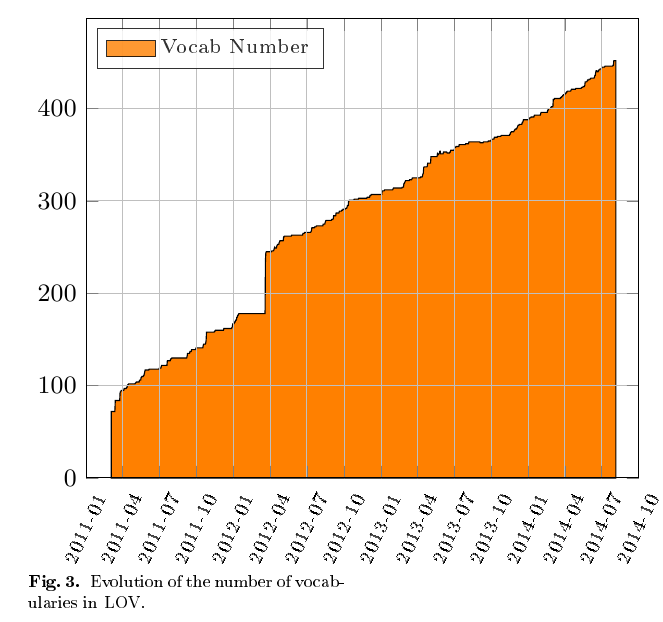
\includegraphics[width=\linewidth]{img/LOVEvol.png}
  \caption{Graph evolution of vocabularies inserted into LOV since from 2011 to 2014.}
  \label{fig:translations}
\end{figure}

LOV focuses only on vocabularies (subpart of semantic documents of the web) submitted by any user, reviewed and validated by curators. In addition, LOV keeps track of different versions of the vocabularies in the server that can be retrieved for comparing the differences between along the time evolution.  In contrast, Swoogle is designed to automatically discover Semantic Web Documents (SWDs), indexes their metadata and answers queries about it. Thus, the result of a search query retrieved any semantic document. For example, a query of the term \textit{person} gives $16,438$ results while in LOV, only the term appears in $134$ vocabularies. 
Watson works similarly to Swoogle, crawling and indexing semantic document at a small scale, explicitly distinguishing for each document (resource), concepts, properties and individuals if available. While in Swoogle  the ranking score is displayed, Watson shows the language of the resource and the size. Falcons is a keyword-based search system for concepts and objects on the Semantic Web, and is equipped with entity summarization for browsing. It is notable that Falcons limits the search only to ontologies and a recommendation feature is provided according to users' preferences. However, it does not provide any relationships between the related ontologies, nor any domain classification of the vocabularies.   
Table \ref{tab:lovfeatures} lists some key features of LOV with respect to Swoogle, Watson and Falcons.
 \begin{table}[!htb]
\centering{
\begin{tabular}{lllll}
\specialrule{1pt}{1pt}{1pt}
 \textbf{Feature}	& Swoogle & Watson & Falcons & LOV 			 \\ \specialrule{1pt}{1pt}{1pt}
Browsing ontologies	   & Yes & Yes & Yes & Yes \\ 
Scope & SWDs & SWDs & Concepts & ontologies \\
Metrics	& Ranking & Ranking & Ranking &  LOD popularity	 \\ 
Domain filtering & No & No & No & Yes \\
Comments and review 	& No & Yes & No & Only by curators	\\ 
Ranking	& Doc. based & Doc. based & Doc. based & Metric-based			\\ 
Web service access & Yes & Yes & Yes & Yes		\\ 
SPARQL endpoint	& No & No & No & Yes		\\ 
Read/Write	& Read & Read \& Write & Read &Read  	\\ 
Ontology directory & No & No & No &Yes \\
Application platform & No & No & No & Yes \\
Storage & Cache & - & - & Dump \& endpoint \\
Interaction with Contributors & No &  - & No & Yes \\

		\\ \specialrule{1pt}{1pt}{1pt}

\end{tabular}
\caption{Comparison of LOV, with respect to Swoogle, Watson and Falcons; based on part of the framework defined in \cite{AquinJoWS12}.  }
\label{tab:lovfeatures}
}
\end{table}


\subsection{LOV vs Neon Methodology}
\label{sec:Lovandneon}

 LOV is a catalog/tool that can fits well within the Neon methodology for building vocabularies and ontologies.  Based on the Neon Methodology's glossary of activities for building ontologies \cite{MC10}, LOV is relevant in four activities:
		
\begin{description}%[fragile]
		\item [Ontology Search.] Main LOV's feature is the search of vocabulary terms. These vocabularies are categorized within LOV according to the domain they address. In this way, LOV contributes to ontology search by means of (a) keyword search and (b) domain browsing.
		\item [Ontology Assessment.] LOV provides a score for each term retrieved by a keyword search. This score can be used during the assessment stage and includes a unique term statistical feature\footnote{\url{http://lov.okfn.org/dataset/lov/stats/}} which provides for each term registered in LOV the following information: (a) ``LOV distribution'' that represents the number of vocabularies in LOV that refer to a particular element; (b) ``LOV popularity'' that shows the number of other vocabulary elements that refers to a particular one; and (c) ``LOD distribution'' that refers to the number of datasets in LOD which use a particular vocabulary; and (d) ``LOD popularity'' that refers to the number of vocabulary element occurrences in the LOD.
		\item [Ontology Mapping.] As explained in section \ref{voafRelations}, vocabularies rely on each other in seven different ways. In LOV these relationships are explicitly stated using VOAF vocabulary. This data could be useful to find alignments between ontologies, for example one user might be interested in finding equivalent classes for a given class or all the equivalent classes among two ontologies. The following example shows the retrieved data when asking for all the equivalent classes and properties between the vocabularies foaf and dcterms by means of the related VOAF query\footnote{\url{http://goo.gl/sTIGQ6}. Prefixes are omitted for readability purpose. You can find the correct namespace for a prefix in LOV.}: 
				
		{\small\begin{verbatim}SELECT DISTINCT ?elem1 ?alignment ?elem2 {
				     {?elem1 <http://www.w3.org/2002/07/owl#equivalentClass> ?elem2}
				     UNION {?elem1 <http://www.w3.org/2002/07/owl#equivalentProperty> ?elem2}
				     UNION {?elem2 <http://www.w3.org/2002/07/owl#equivalentClass> ?elem1}
				     UNION {?elem2 <http://www.w3.org/2002/07/owl#equivalentProperty> ?elem1}
				     FILTER(!isBlank(?elem2))
				     FILTER(!isBlank(?elem1))
				     ?elem1 ?alignment ?elem2.
				     ?elem1 rdfs:isDefinedBy <http://xmlns.com/foaf/0.1/>.
				     ?elem2 rdfs:isDefinedBy <http://purl.org/dc/terms/>.
				} ORDER BY ?alignment\end{verbatim}}
				
	Figure \ref{fig:eqCR} shows the alignments between foaf and dcterms vocabularies by mean of \url{owl:equivalentClass} and \url{owl:equivalentProperty}. 

\begin{figure}
\centering
  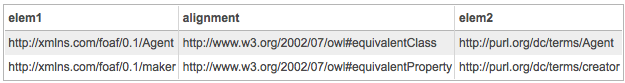
\includegraphics[width=1.0\linewidth]{img/equivalentCandR.png}
  \caption{Equivalent classes and properties between foaf and dcterms}
  \label{fig:eqCR}
\end{figure}

							
		\item [Ontology Localization.] Labels in different languages are stored in the LOV endpoint for the ontology terms that provide such information. This annotations could be used when translating terms into different languages. This information could be extracted by querying the SPARQL endpoint as in the following example\footnote{\url{http://goo.gl/JJCJ01}} where all the labels defined for the terms that have at least one \url{rdfs:label} containing strictly ``person":
		
		{\small\begin{verbatim}SELECT DISTINCT ?label2 ?element{
								     ?element rdfs:label ?label1 .
								     ?element rdfs:label ?label2 .
								     FILTER (?label1 != ?label2 ).
								     FILTER(REGEX(STR(?label1), "person", "i")).
					} ORDER BY ?element\end{verbatim}}
						 
								     
		An excerpt of the query result is shown in figure \ref{fig:translations}. From that result, ``Persona''@es and ``Personne''@fr could be used as translations for the English term ``Person'' in Spanish and French respectively.


\begin{figure}
\centering{
  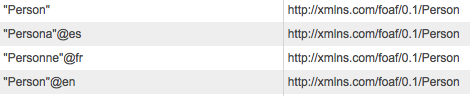
\includegraphics[width=.90\linewidth]{img/translations1.png}
  \caption{Translations example for foaf:Person}
  \label{fig:translations}
  }
\end{figure}

\end{description}

		Figure \ref{fig:LOVandNeOn} shows the activities LOV can support within the overall Neon methodologies activity workflow.
		
\begin{figure}
\centering
  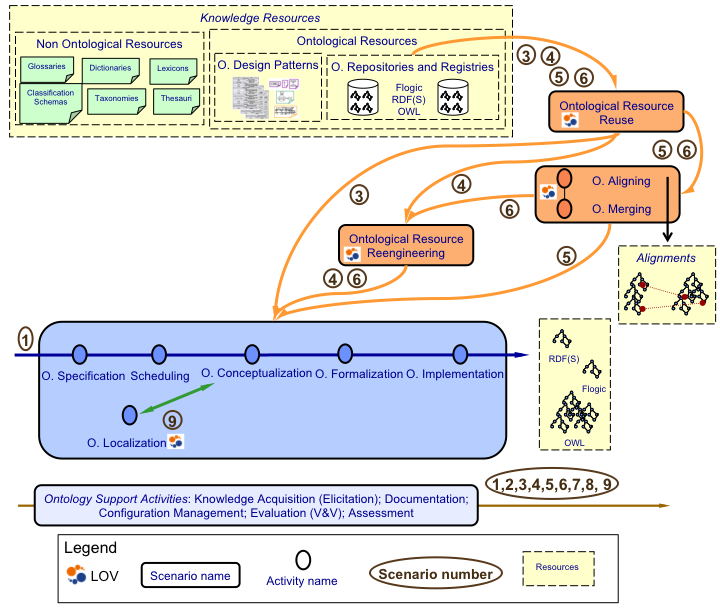
\includegraphics[width=.95\linewidth]{img/neonScenarios.png}
  \caption{Meeting points between LOV and the NeOn methodology, derived from \cite{MC10}.}
  \label{fig:LOVandNeOn}
\end{figure}


\section{Prefixes harmonization}
\label{sec:prefharmoni}

RDF vocabularies bring their meaning to linked data by defining classes and properties, and their formal semantics. Relying on W3C standards RDFS or OWL, those vocabularies are a fundamental layer in the architecture of the Semantic Web. Without the explicit semantics declared in vocabularies, linked data, even using RDF, would be just linked pieces of information where links have no meaning. Interoperability between data and datasets rely heavily on shared vocabularies, but given the distributed nature of the Web, vocabularies are published by independent parties and there is no centralized coordination of this publication, nor should it be. Various independent services have been developed in order to discover vocabularies and provide information about them, and the community of data publishers and vocabulary managers have all interest in complementarity and coordination between such services. In this section, we focus on a specific aspect of vocabularies: their identification by namespaces and associated prefixes.

In the original XML syntax of RDF, prefixes are simply local shortcuts associated with XML namespaces using \texttt{xmlns} declarations. The usage of prefixes has been further extended to other syntaxes of RDF such as N3 and Turtle. Although a prefix to namespace association is syntactically limited to the local context of the file in which it is declared, common prefixes such as \texttt{rdf:}, \texttt{rdfs:}, \texttt{owl:}, \texttt{skos:}, \texttt{foaf:} and many more have become de facto standards. For example, RDFa has 1.1 has a default profile made of 11 well-used vocabularies based on their general usage on the Semantic Web according to the crawl of Yahoo! and Sindice as of March 2013\footnote{\url{http://www.w3.org/2010/02/rdfa/profile/data/}}. Similarly, the YASGUI SPARQL editor has a list of built-in prefix-namespace associations to ease the construction of SPARQL queries. However, this list of ``standard'' prefixes is open-ended. Interfaces such as SPARQL endpoints (e.g. Virtuoso) use a list of built-in prefixes declaration for more and more namespaces but the choice of entries in this list is all but transparent. Hence, the reason of a given namespace being or not in this list could be interpreted in many ways, a potential source of technical and social conflicts. Therefore, the notion has been slowly spreading, at least implicitly, that common prefixes could and indeed should have a global use, implying some kind of governance and good practices. More and more vocabularies explicitly recommend the prefix that should be used for their namespace, generally using a common if not written good practice to avoid frontal clashes by recommending a prefix not already used. But there is no global policy except implicit rules of fair use to avoid potential conflicts resulting from polysemy (different namespaces using or recommending the same prefix) or synonymy (different prefixes used for the same namespace).

A vocabulary publisher needs to have access to some services capable of monitoring the existing prefixes usage in order to stick to those rules. Moreover, we focus on two services providing such information on prefixes usage namely prefix.cc\footnote{Service: \url{http://prefix.cc/}; Code: \url{https://github.com/cygri/prefix.cc}} and LOV (Linked Open Vocabularies)~\cite{Datalift:D22}. Both services provide associations between prefixes and namespaces but following a different logic. The prefix.cc service allows anybody to suggest a prefix to namespace association. It supports polysemy and synonymy, and has a very loose control on its crowd-sourced information. What it provides is more a measure of popularity of prefixes and namespaces than a way to put order in them. LOV has a much more strict policy forbidding polysemy and synonymy, enforced by a dedicated back-office database infrastructure, ensuring that each vocabulary in the LOV database is uniquely identified by a prefix, this unique identification allowing the usage of prefixes in various LOV publication URIs. This requirement leads sometimes to a situation where LOV uses prefixes different from the ones recommended by the vocabulary publishers.

\subsection{Aligning LOV with Prefix.cc} \label{sec:alignment}
In this section, we present how we perform the alignment between the two services LOV and prefix.cc. Figure~\ref{fig:evolution} shows the evolution of the number of prefixes registered in these two services between April 2009 and July 2013. Our main goals are to align Qnames (prefix) to a unique URI in LOV and to make sure that all the vocabularies in LOV are actually inserted in prefix.cc.

\begin{figure}[ht]
\centering
\resizebox{\textwidth}{!}{
%\documentclass{standalone}
%\usepackage{pgfplots}
%\begin{document}
\begin{tikzpicture}
\begin{axis}[
%\begin{semilogxaxis}[
 cycle list name=exotic,
 ylabel=number of prefix-namespace,
 xlabel=month,
% legend pos=outer north east,
 legend style={at={(0.02,0.98)},anchor=north west,opacity=0.6},
% legend columns=2,
 axis on top,
 ymin=0,ymax=1300,
 mark size=0pt,
 grid=major,
% minor x tick num=10,
% minor y tick num=10,
%xtick={Jan-09,Feb-09,Mar-09,Apr-09,May-09,Jun-09,Jul-09,Aug-09,Sep-09,Oct-09,Nov-09,Dec-09,Jan-10,Feb-10,Mar-10,Apr-10,May-10,Jun-10,Jul-10,Aug-10,Sep-10,Oct-10,Nov-10,Dec-10,Jan-11,Feb-11,Mar-11,Apr-11,May-11,Jun-11,Jul-11,Aug-11,Sep-11,Oct-11,Nov-11,Dec-11,Jan-12,Feb-12,Mar-12,Apr-12,May-12,Jun-12,Jul-12,Aug-12,Sep-12,Oct-12,Nov-12,Dec-12,Jan-13,Feb-13,Mar-13,Apr-13,May-13,Jun-13,Jul-13,Aug-13},
xtick={Jan-09,Apr-09,Jul-09,Oct-09,Jan-10,Apr-10,Jul-10,Oct-10,Jan-11,Apr-11,Jul-11,Oct-11,Jan-12,Apr-12,Jul-12,Oct-12,Jan-13,Apr-13,Jul-13},
 ytick={0,100,...,1300},
 symbolic x coords={Jan-09,Feb-09,Mar-09,Apr-09,May-09,Jun-09,Jul-09,Aug-09,Sep-09,Oct-09,Nov-09,Dec-09,Jan-10,Feb-10,Mar-10,Apr-10,May-10,Jun-10,Jul-10,Aug-10,Sep-10,Oct-10,Nov-10,Dec-10,Jan-11,Feb-11,Mar-11,Apr-11,May-11,Jun-11,Jul-11,Aug-11,Sep-11,Oct-11,Nov-11,Dec-11,Jan-12,Feb-12,Mar-12,Apr-12,May-12,Jun-12,Jul-12,Aug-12,Sep-12,Oct-12,Nov-12,Dec-12,Jan-13,Feb-13,Mar-13,Apr-13,May-13,Jun-13,Jul-13,Aug-13},
 xmin=Feb-09,xmax=Aug-13,
 x tick label style={rotate=65,anchor=east,font=\scriptsize}
 ]
  
\pgfplotstableread{PGFPlots/prefixcc-lov-evo.dat}\thisTable
%\pgfplotstableread{prefixcc-lov-evo.dat}\thisTable

\addplot table[x=month,y=prefix.cc]{\thisTable};
\addlegendentry{prefix.cc}

\addplot table[x=month,y=LOV]{\thisTable};
\addlegendentry{LOV}

%\end{semilogxaxis}
\end{axis}
\end{tikzpicture}
%\end{document}
}
\vspace{0.1cm}
\caption{Evolution of the number of prefix-namespace pairs registered in prefix.cc and LOV}
\label{fig:evolution}
\end{figure}

We propose to perform SPARQL queries over all the files of prefix.cc at\\
 \url{http://prefix.cc/popular/all.file.vann} in the FROM clause and compare them to the content of the LOV SPARQL endpoint\footnote{\url{http://lov.okfn.org/endpoint/lov}} via a SERVICE\footnote{\url{http://www.w3.org/2009/sparql/docs/fed/service}} call. The SERVICE keyword defined in the SPARQL 1.1 Query Language instructs a federated query processor to invoke a portion of a SPARQL query against a remote SPARQL endpoint~\cite{eric2013}. Results are returned to the federated query processor and are combined with results from the rest of the query. To be more generic and standards-compliant, the queries could be run with the Jena ARQ command-line tool to produce a CSV or a JSON serialization that could be easily consumed either by the prefix.cc backend via phpMyAdmin or by the LOV backend.

\subsection{First Task: prefixes in LOV not present in Prefix.cc}  \label{sec:notInPrefix}
First, we compute $<LOV> INTERSECTS <PREFIX.CC>$ and $<LOV> MINUS \, \{<LOV> INTERSECTS <PREFIX.CC> \}$. The following SPARQL query finds namespace URIs in LOV that do not exist in prefix.cc along with their LOV prefix.
\begin{verbatim}
PREFIX vann: <http://purl.org/vocab/vann/>
SELECT ?prefix ?lovURI
FROM <http://prefix.cc/popular/all.file.vann> {
  SERVICE <http://lov.okfn.org/endpoint/lov> {
    SELECT ?prefix ?lovURI {
      [] vann:preferredNamespacePrefix ?prefix;
        vann:preferredNamespaceUri ?lovURI;
    }
  }
  FILTER (NOT EXISTS { [] vann:preferredNamespaceUri ?lovURI })
  OPTIONAL {
    [] vann:preferredNamespacePrefix ?prefix;
      vann:preferredNamespaceUri ?pccURI;
  }
}
ORDER BY ?prefix
\end{verbatim}
The first results\footnote{This query was performed in two weeks between March, 2nd and March, 20th 2013 and at this time, card(LOV) = 321 vocabularies while card(Prefix.cc) = 925} shown the following: $card(LOV) \bigcap card(PREFIX.cc) = 188$\footnote{\url{http://www.eurecom.fr/~atemezin/iswc2013/experiments/firstAlignments/intersection-prefixLOV-02-03.csv}} and $card (LOV) - card( PREFIX.cc) = 133$\footnote{\url{http://www.eurecom.fr/~atemezin/iswc2013/experiments/firstAlignments/inLovNotINPrefixcc-02-03.csv}} prefixes in LOV not yet registered in prefix.cc. At this point, a first batch of $80$ prefixes/namespaces from LOV were safely imported in prefix.cc since there were no conflicts. For the remaining conflicting ones, they needed more in-depth analysis.

\subsection{Second Task: Dealing with Conflicts between Prefix.cc and LOV}  \label{sec:conflicts}
In the process of alignment, there were two types of conflicts and we provide appropriate actions and/or solutions accordingly:
\begin{itemize}
 \item Clashes: cases where we have in both services the same prefix but different URIs;
 \item Disagreements on preferred namespace: cases where for the same URI, we found different prefixes.
\end{itemize}

\subsubsection*{Clashes.} We performed a SPARQL query as above to identify clashes in vocabularies ($30$). In Table~\ref{tab:clashes-types}, we identify seven different types of issues to deal with, such as (i) real conflicts, (ii) URIs are 404, (iii) URIs are obsolete versions and (iv) two URIs redirecting to the same resource.
\begin{table}
\centering{
\begin{tabular*}{14cm}{lcl}
\specialrule{1pt}{1pt}{1pt}
 \textbf{Type of issue}	& \textbf{\# Vocabularies} 	& \textbf{\%} 		 \\
 \specialrule{1pt}{1pt}{1pt}
 pccURI and lovURI redirect to same resource  & 8 	& 26.67\%		\\
 lovURI already in prefix.cc as secondary	  & 7   & 23.3\%  		\\
 Real conflicts 	                & 6 			& 20\% 	 		\\
 pccURI is 404	                    & 4 			& 13.3\%		\\
 pccURI is an obsolete version		& 3   			& 10\%  		\\
 lovURI is 404		                & 1   			& 3.3\%  		\\
 lovURI is an obsolete version		& 1   			& 3.3\%  		\\
 \specialrule{1pt}{1pt}{1pt}
\end{tabular*}
\caption{Type of issues encountered for vocabulary clashes}
\label{tab:clashes-types}
}
\end{table}

\subsubsection*{Disagreements on namespace URIs.} The general idea is that if vocabulary editors have not included explicitly a \\ \texttt{vann:preferredNamespacePrefix} in their description, the curators of LOV are free to change it and put whatever seems appropriate. At the same time, in prefix.cc, having multiple prefixes for the same namespace IRI in not a problem. However, we computed those prefixes in LOV that have different prefixes in prefix.cc. The following query retrieves the URIs falling in those disagreements:
\begin{verbatim}
PREFIX vann: <http://purl.org/vocab/vann/>
SELECT ?prefix ?lovURI ?prefixcc
FROM <http://prefix.cc/popular/all.file.vann> {
  SERVICE <http://lov.okfn.org/endpoint/lov> {
    SELECT ?prefix ?lovURI {
      [] vann:preferredNamespacePrefix ?prefix;
        vann:preferredNamespaceUri ?lovURI;
    }
  }
  FILTER (?pccURI = ?lovURI && ?prefix != ?prefixcc)
  OPTIONAL {
    [] vann:preferredNamespacePrefix ?prefixcc;
      vann:preferredNamespaceUri ?pccURI;
  }
}
ORDER BY ?prefix
\end{verbatim}
From the results of this query ($61$ cases), we have three actions to perform:
\begin{itemize}
  \item add the lovPrefix (prefix in LOV) in prefix.cc (e.g: adding \\\texttt{geod}:\texttt{http://vocab.lenka.no/geo-deling\#}) to the existing \texttt{ngeoi} in \textit{pccPrefix}.)
  \item add more alternative URIs to the existing prefix in prefix.cc (e.g: adding \texttt{prov}:\texttt{http://purl.org/net/provenance/ns\#}) to the existing \texttt{hartigprov, prv} in \textit{pccPrefix})
  \item change a prefix in LOV\footnote{\url{http://www.eurecom.fr/~atemezin/iswc2013/material/action-sameUriDifferentPrefixes.pdf}} (e.g: lovPrefix \texttt{dc} for \texttt{http://purl.org/dc/terms} not in the list $\{dcterm, dcq, dct, dcterms\}$ has been replaced by \texttt{dce} in LOV).
  \item No changes when the lovPrefix is contained in the set of prefixes of prefix.cc.
\end{itemize}

\subsection{Social Aspects} \label{sec: social}
Several vocabularies are maintained by a community of users. As part of the alignment process, we contacted the authors, creators or maintainers (if they exist) of vocabularies to involve them as well in the process of changing prefixes, and agree with them to fix some issues regarding their vocabularies. From the homepages of the vocabulary authors and editors collected in LOV, we connect to their social platform accounts such as LinkedIn, Google+ or Twitter. Table~\ref{tab:contact-editors} summarizes some cases of real conflicts where the LOV curators have to find and contact the editors of the vocabularies for negotiation.

\begin{table}[htp]
\centering{
\begin{tabular*}{12cm}{lll}
 \specialrule{1pt}{1pt}{1pt}
 prefix & lovURI		& Remark \\
 \specialrule{1pt}{1pt}{1pt}
 sp & \scriptsize{http://data.lirmm.fr/ontologies/sp\#} &	 contact editor at LIRMM ($sp \Rightarrow osp$) \\  %\scriptsize{http://spinrdf.org/sp\#}
 scot & \scriptsize{http://scot-project.net/scot/ns\#} &  contact editors at lovURI \\   % \scriptsize{http://scot-project.org/scot/ns\#} &
 media &	\scriptsize{http://purl.org/media\#}	 & contact editors for negotiation \\ %& \scriptsize{http://purl.org/microformat/hmedia/}
 pro	& \scriptsize{http://purl.org/spar/pro/}  &  contact editors for negotiation \\   % &	\scriptsize{http://purl.org/hpi/patchr\#}
 swp	& \scriptsize{http://www.w3.org/2004/03/trix/swp-1/}  & contact editors, fix on LOV side \\  %& \scriptsize{http://www.w3.org/2004/03/trix/swp-2/}
 wo & \scriptsize{http://purl.org/ontology/wo/core\#}	 & contact editors \\  %& \scriptsize{http://purl.org/ontology/wo/}
 idemo &	\scriptsize{http://rdf.insee.fr/def/demo\#}	 & to resolve with INSEE \\ %& \scriptsize{http://rdf.insee.fr/graphes/def/demo\#}
 \specialrule{1pt}{1pt}{1pt}
\end{tabular*}
\caption{LOV and prefix.cc conflicts resolution leading to contact vocabularies editors for negotiation. We provide the prefix, the URI in LOV and the action undertaken.}
\label{tab:contact-editors}
}
\end{table}

%%%%%%%%%%%%%%%%%%%%%%%%%%%%%%%%%%%%%%%%%%%%%%
%%%  4. Finding Vocabularies in Prefix.cc  %%%
%%%%%%%%%%%%%%%%%%%%%%%%%%%%%%%%%%%%%%%%%%%%%%

\subsection{Finding Vocabularies in Prefix.cc}   \label{sec:finding}
We want to find out in prefix.cc, which of the couples (prefix, URI) could be potentially a vocabulary to be further assess to be included in the LOV catalog. To address this question, we first compute all the differences on prefix.cc NOT in LOV, i.e. $PREFIX.CC$ MINUS $(LOV <INTERSECT> PREFIX.CC)$, performing using a SPARQL query. This results in $742$ URIs to be checked\footnote{\url{http://www.eurecom.fr/~atemezin/iswc2013/experiments/input/notInLOV.json}}.

\subsubsection{LOV Check API}
We have implemented an API\footnote{\url{http://lov.okfn.org/dataset/lov/apidoc/}} that allows a user to run the LOV-Bot over a distant vocabulary. It takes as parameter the vocabulary URI to process and the time out (integer) specified to stop the process. The result of this action is a set of $26$ property-values from which we are interested in using only $8$ of them, namely:
\begin{itemize}
 \item \textbf{uri} (string); uri of the vocabulary.
 \item \textbf{namespace} (string) ; namespace of the vocabulary.
 \item {\textbf{prefix} (string) ;  prefix of the vocabulary}
 \item{\textbf{inLOV} (boolean) ; indicates if the vocabulary is already in the Linked Open Vocabularies ecosystem}.
 \item {\textbf{nbClasses} (int) ; Number of classes defined in the vocabulary namespace}.
 \item{\textbf{nbProperties} (int) ; Number of properties defined in the vocabulary namespace}.
 \item{\textbf{dateIssued }(string) ; Vocabulary date of issue}.
 \item{\textbf{title} (Taxonomy) ; List of titles with language information if available}.
\end{itemize}

The code below gives the response of our algorithm for the vocabulary identified at \url{http://ns.aksw.org/Evolution/}.
\begin{verbatim}[caption={Sample output of a response of the Check API}]
{
 "dateIssued": "None",
 "inLOV": false,
 "namespace": "http://www.agfa.com/w3c/2009/clinicalProcedure#",
 "nbClasses": 47,
 "nbProperties": 29,
 "pccURI": "http://www.agfa.com/w3c/2009/clinicalProcedure",
 "prefix": "clinproc",
 "title": [
   {
     "dataType": null,
     "language": "en",
     "value": "Clinical Procedure"
   }
 ],
 "uri": "http://www.agfa.com/w3c/2009/clinicalProcedure"
},
\end{verbatim}

\subsubsection{Experiments} \label{experiments}
We wrote a script calling the LOV Check API on the URIs in prefix.cc for determining the candidates vocabularies to be inserted in LOV using the algorithm in Listing~\ref{findvocabInPrefix-algorithm}. We ran four times the experiments (possibly due to some network instabilities) in order to determine from which results what should be assessed. Table~\ref{tab:experiment-choice} gives an overview of the number of URIs with respectively the attribute ``inLOV=false''(TP), ``inLOV=true''(FP) and the errors occurred (Null returned, http/proxy or time out reached by the API).

Regarding the experiments, \texttt{Experiment4} gives stable results with less network errors. Therefore, we stick on this experiment to report our findings and analysis. We found that $227$ ($43.48$\%) are vocabularies in the sense of LOV since they have at least one property or one class. $297$ vocabularies ($56.51$\%) might have some problems (or are even not vocabularies at all) as they have neither classes nor properties. Regarding the presence of prefixes, we found $140$ ($61.67$\%) of them.
\begin{table}[!htbp]
\centering{
\begin{tabular}{lccc}
 \specialrule{1pt}{1pt}{1pt}
 				& TP(inLOV=false) 	& FP(inLOV=true) 	& Errors	 \\
 \specialrule{1pt}{1pt}{1pt}
 Experiment1 	& 525 				& 44 				& 173 		 \\
 Experiment2 	& 403 				& 26				& 313 		 \\
 Experiment3 	& 351 				& 28				& 363 		 \\
 Experiment4	& $522$   			& 44   				& 176 		 \\
 \specialrule{1pt}{1pt}{1pt}
\end{tabular}
\caption{Experiments looking for stable results of finding vocabularies in prefix.cc.}
\label{tab:experiment-choice}
}
\end{table}
The $227$ vocabularies could all be inserted in the LOV catalog since they fulfill the current requirements of what is a `` LOV-able vocabulary''. In this list, we found vocabularies such as \texttt{rdf, rdfs, owl} that are used to build other vocabularies but are not yet integrated in the LOV catalog.

\begin{algorithm}[H]
\caption{finding vocabularies NOT in LOV from prefix.cc algorithm} \label{findvocabInPrefix-algorithm}
\begin{algorithmic}[1]
    \STATE Open $notInLOV.json$ file containing the prefix.cc URIs \NOT in LOV 
    \STATE initialize $item$ as List
    \STATE Initialize $result$ as collection of $item$
    \FOR { each $pccURI \in notInLOV file$}
      \STATE $uri \leftarrow$ value of $pccURI$
      \STATE $uriv \leftarrow$ construct-valid $uri$
      \STATE call LOV-Check API with parameter $uriv$
      \STATE try/catch HTTPError, URLError, IOError, ValueError
      \WHILE { no error raised}
        \STATE initialize $item$ to an empty List
        \STATE append $pccURI, prefix, inLOV, namespace, title, dateIssued, nbClasses, nbProperties$ in $item$ List
        \STATE append $item$ to $result$
      \ENDWHILE
    \ENDFOR
    \PRINT $output-result$
\end{algorithmic}
\end{algorithm}

From the list of URIs that were not LOV-able vocabularies, we wanted to do more analysis by checking the RDF files using the Triple-Checker tool. Our aim is to be sure if we did not leave out some candidate vocabularies or if there are other type of errors such as parsing errors. Table~\ref{tab:triplechecker-analysis} provides results classified into $4$ categories:
\begin{itemize}
 \item General errors such as loading files or proxy errors: 78.30\%
 \item Candidate LOV-able vocabularies: 12.20\%
 \item Clearly not vocabularies ($\texttt{nbClasses} = \texttt{nbProperties} = 0 $), typically instances, datasets, html pages: 6.45\%
 \item Others (mainly parsing errors): 3.05\%
\end{itemize}

\begin{table}
\centering{
\begin{tabular}{lccc}
 \specialrule{1pt}{1pt}{1pt}
 \textbf{Total URIs }				& $295$ & 100\% 		\\
 \specialrule{1pt}{1pt}{1pt}
 Loading/404 errors			        & $182$ & 61.69\%		\\
 Vocabularies 						& 36 	& 12.20\% 		\\
 Proxy errors				        & 27   	& 9.15\%   		\\
 50x, 40x errors				    & 22   	& 7.45\%   		\\
 Parsing errors				        & 9   	& 3.05\%   		\\
 Web Pages containers				& 9   	& 3.05\%   		\\
 No triples found				    & 8   	& 2.71\%   		\\
 RDF data 						    & 2 	& 0.67\%		\\
\specialrule{1pt}{1pt}{1pt}
\end{tabular}
\caption{Analysis of the URIs with no classes and no properties while using the LOV-Bot API}
\label{tab:triplechecker-analysis}
}
\end{table}

\subsection{Conclusion}    \label{sec:conclusion}
In this Section, we have analyzed numerous vocabularies referenced in LOV and in prefix.cc and we have presented a way to manage the prefixes of those vocabularies. We have shown that in the process of mapping namespaces with prefixes, some conflicts have to be resolved, often by contacting the editors themselves. One future work is to develop a new strategy for the LOV-Bot API to take into account vocabularies published in other formats such as n3 and turtle. This would require to first test the validity of those formats and to adapt the way namespaces are obtained in order to not check only the presence of the \texttt{vann:preferredNamespace} property but to rely on similarity algorithm in order to guess the closest namespace given a URI vocabulary and some statistics of the number of classes and properties.

The work can be extended in several directions. Sticking to the two services we have studied and already contributed to harmonize, the possible next steps would be to automate as far as possible the tasks that have been made semi-automatically so far: \emph{i)} developing a unique interface for submitting namespaces and prefixes to both services; \emph{ii)} bridging the LOV back-office and the prefix-cc database using both services API in order to publish a list of common recommended prefixes. The latter goes beyond the limited framework of the two original services since such a list could be consolidated and endorsed by the main actors in vocabulary publication and management, and recommended for use in linked data applications. This could be picked up by the upcoming W3C Vocabulary Management Working Group as part of the new Data Activity\footnote{\url{http://www.w3.org/2013/05/odbp-charter.html}}.
 
This (apparently) simple issue of prefixes and namespaces is providing a good illustration of why some kind of governance is needed in the distributed ecosystem of vocabularies and linked data, pointing to both technical and social aspects, and proposing concrete examples of conflict resolution. There is no, and certainly there should never be any, central attribution authority for prefixes, and the needed regulation has to be made a posteriori, including good practices of cooperation and negotiation between vocabulary publishers. Development and harmonization of services such as LOV and prefix.cc is then to be considered as part of the current and more general effort already started by the DCMI\footnote{Long-term Preservation and Governance of RDF Vocabularies: \url{http://dcevents.dublincore.org/IntConf/index/pages/view/vocPres}} and W3C\footnote{W3C Vocabulary Services: \url{http://www.w3.org/2013/04/vocabs/}} for a sustainable governance of vocabularies.

\section{Vocabulary Ranking metrics}
\label{sec:vocabranking}

\label{sec:introduction}
The linked data principles have gained significant momentum over the last few years as a best practice for sharing and publishing structured data on the Semantic Web~\cite{Bizer2009}. Before being published, data is modeled and ontologies or vocabularies are one of the key elements of a dataset. Vocabularies are the artefact that bring semantics to raw data. One of the major barriers to the deployment of linked data is the difficulty for data publishers to determine which vocabularies should be used since developing new vocabularies has a cost. Catalogues of ontologies are therefore a useful resource for searching terms (classes and properties) defined in those vocabularies. The Linked Open Vocabulary (LOV) initiative~\cite{scharffe_2012} is playing a significant role in providing such services to users who can search within curated vocabularies, fostering ontologies reuse. LOV focuses only on vocabularies submitted by users, which are then reviewed and validated by curators. In addition, LOV computes dependencies between vocabularies, keeps track of different versions of them in order to enable their temporal evolution.

To the best of our knowledge, recommending vocabularies to reuse are limited to ``popular'' or ``well-known'' ones. This paper proposes a metric combining different features such as how vocabularies are interlinked, or how they are used in real world datasets. This contribution originates also in the desire to bring the traditional concept of Information Content (IC) into the field of the semantic web applied to vocabularies. Many catalogs of ontologies already provide some ranking metrics based on some features. However, we are interested in applying the principles of IC on vocabularies to investigate if such techniques can give more insights in ontology ranking and ontology usage (e.g in visualization applications).

This Section is organized as follows: Section~\ref{sec:theory} defines the theory of Information Content, and the features used for applying Partition Information Content to vocabularies. We present our experiments on the LOV catalogue in the Section~\ref{sec:experiments}. We discuss how this ranking metric can be used for vocabulary design and maintenance in Section~\ref{sec:application}. We compare our results with other rankings for vocabularies in Section~\ref{sec:related} before concluding and outlining future work (Section~\ref{sec:conclusion}).



\subsection{Information Content Metrics}
\label{sec:theory}
Based on probability theory, Information Content (IC) is computed as a measure of generated amount of surprise~\cite{ross02}. More common terms in a given corpus with higher chance of occurrence cause less surprise and accordingly carry less information, whereas infrequent ones are more informative. We reuse the notion of informativeness as the value of information associated with a given entity, where Information Content has a negative relation with its probability. The concept of Information Content can be used to rank each entity, term, or alphabet in the corpus. We apply the Partitioned Information Content to measure the informativeness of Linked Open Vocabularies as a semantic network of resources connected together using different range of relations, as described in~\cite{Meymandpour13}. Partitioned Information Content (PIC) is derived from the IC value using some weights. We empirically set those weights according to three features:
\begin{itemize}
 \item (i) datasets using the vocabulary ($weight = 2$);
 \item (ii) \textit{outlinks} from a vocabulary, i.e. whether a vocabulary reused other vocabularies ($weight = 1$);
 \item (iii) \textit{inlinks} to a vocabulary, i.e. whether other vocabularies are reusing this vocabulary ($weight = 3$).
\end{itemize}

\subsection{Information Content in Linked Open Vocabularies}
This experiment aims at bringing the concept of informativeness in the field of terms semantically related as it is the case within semantic web ontologies. The ranking obtained can give additional information based on the Information Content theory to help reusing terms and detecting the ones that are less popular. This can then be used by applications consuming datasets described with these vocabularies. The equation (1) gives the formula for computing the IC value of a term (class or property):
\begin{equation}
 IC(t) = -\log_2(\frac{\varphi(t)}{N}) ,
\end{equation}
where $N$ is set to be the maximum value corresponding to the term occurrence in the LOV aggregator (as of June 2014, this value is $3958$, and it corresponds to the popularity of the \texttt{skos:prefLabel} property); and $\varphi(t)$ is the occurrence of the term (but not its popularity).

For computing $\varphi(t)$, we use two types of SPARQL queries depending on whether the term is a class (Listing~\ref{list:classCount}) or a property (Listing~\ref{list:propCount} considers \texttt{owl:ObjectProperty}, \texttt{owl:Data\-typeProperty} and \texttt{rdfs:Property}). Note that we do not yet take into account the \texttt{owl:equivalentClass} and \texttt{owl:equi\-valentProperty} axioms that may appear in some vocabularies. We leave this as a future work.

\begin{lstlisting}[float=htb,caption={SPARQL query for computing the occurrence of a class },label=list:classCount]
 SELECT (count(?uri1) as ?occ)
 WHERE {
   ?uri1  ?p %%classURI . }
\end{lstlisting}

\begin{lstlisting}[float=htb,caption={SPARQL query for computing the occurrence of a property },label=list:propCount]
 SELECT (count(?uri1) as ?occ)
 WHERE {
   ?uri1 +objectURI+ ?uri2.
   FILTER  (?uri1 != ?uri2) }
\end{lstlisting}

\subsection{Ranking Vocabularies using Information Content}
For computing the PIC value, we use the following formula:
\begin{equation}
 PIC(f) =  w_{f} \times \sum_{i=1}^{n}IC(t_{i})  ,
\end{equation}
where $w_{f}$ is the weight related to vocabulary $f$.

We consider very important that a vocabulary is being reused by other vocabularies and implemented within real world datasets. For example, the \texttt{foaf} ontology is weighted $6$ because it reuses vocabularies (1), it has been used in some datasets (2) and it is being reused by other vocabularies (3). The \texttt{dul}\footnote{\url{http://www.ontologydesignpatterns.org/ont/dul/DUL.owl}} vocabulary is weighted $3$ because it doesn't reuse any vocabulary but it is instead used by several other vocabularies.
\vspace{-0.2cm}

%%%%%%%%%%%%%%%%%%%%%%%%%%%%%%%%%%%%%%%%
%%%   Experiments on Vocabularies  %%%
%%%%%%%%%%%%%%%%%%%%%%%%%%%%%%%%%%%%%%%%

\subsection{Experiments on Vocabularies}
\label{sec:experiments}
We use the LOV catalogue, and particularly the LOV aggregator\footnote{\url{http://lov.okfn.org/endpoint/lov_aggregator}} to look at the terms (classes and properties) to compute their Information Content (IC). LOV defines the \textit{LOV Distribution} as the number of vocabularies in LOV that refer to a particular element and the \textit{LOV popularity} as the number of other vocabulary elements that refers to a particular one. Based on the concept of Partitioned Information Content, we implement our ranking measure according to the algorithm~\ref{rankingvocab}. We take the subset of classes and/or properties with LOV popularity and LOV distribution greater than one. The initial set of vocabularies in LOV is $366$. After filtering the candidate terms, we came out with a set of $161$ vocabularies ($44\%$ or $161$ vocabularies) for computing their ranking.

The Table~\ref{tab:top15} gives the Top 15-ranking of the vocabularies according to the informativeness of the classes and properties used within the LOV ecosystem. As the function is proportional to the number of terms, we use a threshold of $22$ terms in the vocabularies. For example, the PIC value of \texttt{dcterms} is higher than \texttt{foaf}'s because the former uses $53$ terms (39 properties and 14 classes), while the latter only $35$ terms (9 classes and 26 properties), although they both have the same weight value.

The Table~\ref{tab:top20} shows the Top 20 namespaces of vocabularies according to the informativeness of the classes and properties used within the LOV ecosystem, along with their Information Content Value.
\begin{table}[htbp]
\centering{
\begin{tabular}{lrcc}
\specialrule{1pt}{1pt}{1pt}
 \textbf{Rank}	& \textbf{Prefix} 	& \textbf{PIC score} 		 \\ \specialrule{1pt}{1pt}{1pt}
1 	& \textsf{dcterms}			& 1724.844	 		 \\
2	& \textsf{schema}		    & 1588.700				 \\
3 	& \textsf{gr} 				& 1261.101		\\
4	& \textsf{foaf}  			& 1033.197 			\\
5	& \textsf{bibo}   			& 876.205  			\\
6	& \textsf{time}   			& 816.2020  			\\
7	& \textsf{skos}   			& 805.287  			\\
8	& \textsf{dul}   			& 797.328  			\\
9	& \textsf{ptop}   			& 773.167  			\\
10	& \textsf{rdafrbr}   		& 640.834 			\\
11	& \textsf{vaem}   		    & 630.621 			\\
12	& \textsf{ma-ont}   		& 508,694 			\\
13	& \textsf{prov}   		    & 497.524 			\\
14	& \textsf{swrc}   		    & 437.394 			\\
15	& \textsf{dce}   			& 428.618  			\\ \specialrule{1pt}{1pt}{1pt}
\end{tabular}
\caption{Top 15 vocabularies according to their PIC. All the prefixes used for the vocabularies are the ones used by LOV}
\label{tab:top15}
}
\end{table}

\begin{table}[htbp]
\centering{
\begin{tabular}{llr}
\specialrule{1pt}{1pt}{1pt}
 \textbf{Rank}	& \textbf{vocab term} & \textbf{IC value} 			 \\ \specialrule{1pt}{1pt}{1pt}
1 	& \textsf{skos:example}	& 7.7806		       	 		 \\
2	& \textsf{dce:contributor} & 4.674						 \\
3 	& \textsf{skos:scopeNote} & 4.365					\\
4	& \textsf{dcterms:source} & 4.299			 			\\
5	& \textsf{mads:code}   	& 3.922		  			\\
6	& \textsf{mads:authoritativeLabel}  & 3.922 			\\
7	& \textsf{vs:userdocs} 	& 3.847		 			\\
8	& \textsf{dce:title}  & 3.79			  			\\
9	& \textsf{skos:hasTopConcept} & 3.4547 		 		\\
10	& \textsf{dce:description} & 2.758 		 		\\
11	& \textsf{dcterms:issued} & 2.553	 		\\
12	& \textsf{dce:creator}	& 2.518 		\\
13	& \textsf{skos:inScheme}	& 2.202 		\\
14	& \textsf{skos:notation}	& 1.924	 		\\
15	& \textsf{dcterms:description} & 1.646		 		\\
16	& \textsf{coll:List}		& 0.761		\\
17	& \textsf{vs:term\_status}	& 0.735	 		\\
18	& \textsf{skos:definition}	& 0.43	 		\\
19	& \textsf{skos:prefLabel} & 0.009	 		\\
20	& \textsf{foaf:Person} & 0		  			\\ \specialrule{1pt}{1pt}{1pt}
\end{tabular}
\caption{Ranking of Top 20 terms (classes and properties) according to their IC value}
\label{tab:top20}
}
\end{table}

\begin{algorithm}[htbp]
\caption{Ranking vocabularies algorithm} \label{rankingvocab}
\begin{algorithmic}[1]
  \footnotesize{  \REQUIRE Dump of $lov aggregator$ file
    \STATE Upload in a triple store for querying
    \STATE Select subset of candidate vocabs $ LOV aggregator endpoint $
    \FOR { $term \in lovaggregator$ }
    	\IF {($LOV distribution \geq 1$ )\AND ($LOV Popularity \geq 1$)}
     		\STATE $candidateterms \leftarrow$ append $term$
       \ENDIF
    \ENDFOR
    \FOR { each $term \in candidateterms$}
	\STATE GROUP BY vocabulary namespace
	\STATE COMPUTE weight for each vocabulary
    \ENDFOR
    \STATE INITIALIZE $PICvector$ AS a vector
     \FOR { each $term \in candidateterms$}
      \WHILE { $term \in vocabularySpace $}
        \STATE $ICterm \leftarrow$ function IC(term, vocabPrefix)
	\STATE $ICvocab \leftarrow$ $\sum ICterm $
       \ENDWHILE
        \STATE  $PICvocab \leftarrow$ $weight(vocab) \times $ICvocab
        \STATE $PICvector \leftarrow$ append (PICvocab)
        \STATE ORDER PICvector
    \ENDFOR
    \RETURN PICvector
  }
\end{algorithmic}
\end{algorithm}

%%%%%%%%%%%%%%%%%%%%%%%%%%%%%%%%%%%%%%%%%%%%%%%%%%%%%%%%%%%%%%%
%%%  4. Application of Information Content on Vocabularies  %%%
%%%%%%%%%%%%%%%%%%%%%%%%%%%%%%%%%%%%%%%%%%%%%%%%%%%%%%%%%%%%%%%

\subsection{Application of Information Content on Vocabularies}
\label{sec:application}
We foresee various applications using the ranking method based on the Information Content metric while designing semantic web applications, vocabulary life-cycle management or novel recommendation services. We make the following recommendations when using the PIC ranking method on vocabularies:
\begin{itemize}
 \item Vocabularies on the Top PIC-ranking can be used in visualization applications, i.e. to be displayed to the user as much as possible.
 \item Terms with lower IC can be used in facetted browsing, and they seem appropriate for generating \texttt{sameAs} links during the interconnection and enrichment process. They might also be used for promoting the reuse of terms in vocabularies in general.
 \item The PIC-ranking could help the ontology designers to monitor and to assess the usage of some terms and lead to update the ontology accordingly. For example, it can be useful in extending the use of the properties such as \texttt{vs:term\_status} or \texttt{owl:deprecated}.
 \item Such a ranking can be used to rank organizations or publishers of vocabularies in a time period (e.g. annual) as a way to encourage good qualities vocabularies and/or datasets on the cloud.
\end{itemize}
The use of the information content on LOV vocabularies can be applied in the datasets interlinking task and visualization applications workflow. For interlinking datasets, this method can help detecting properties with a lower PIC which will be a candidate for the interlinking tool. The PIC score can further be used to track the vocabularies terms status (i.e. \texttt{vs:term\_status} ) or \texttt{owl:deprecated} properties by dataset maintainers. From the list of namespaces having deprecated terms (Table~\ref{tab:deprecated}), we observe some correlations with the PIC rank for the vocabularies \texttt{dcat (8), vcard (36), gr (6), wl (2), pav (1)} and \texttt{bibo (1)}\footnote{As of June 2014, there are 60 terms deprecated in LOV with the query \url{http://bit.ly/1aqcDf3}}. More precisely, the presence of \texttt{gr} and \texttt{bibo} provides evidence of such a correlation, while the presence of \texttt{dcat} and \texttt{card} can be explained by the fact that those two vocabularies are in a review process at W3C and subject to re-modeling respectively. Table~\ref{tab:deprecated} gives an overview of some namespaces with their deprecated terms.



\subsection{Related Work and Discussion}
\label{sec:related}
In this section, we look at three other catalogues providing rankings for vocabularies: vocab.cc, LODStats and prefix.cc. vocab.cc\footnote{\url{http://vocab.cc/v/tco}} does not provide a ranking for vocabularies but rather proposes a rank for classes and properties. The proposed ranking presented in Table~\ref{tab:compareRanking} is taken from the ranking of classes assuming the namespace is used only once per class.

\begin{table}[!htbp]
\centering{
\begin{tabular}{lcc}
\specialrule{1pt}{1pt}{1pt}
 \textbf{prefix}	& \#DeprecatedTerms 	& dcterms:modified		 \\ \specialrule{1pt}{1pt}{1pt}
\textsf{vcard} 	& 36	 & 2013-09-25  \\
\textsf{dcat} 	& 8 & 	2013-09-20  \\
\textsf{gr}	 & 6 & 	2011-10-01  \\ 		
\textsf{wl}	 & 2 & 	2013-05-30  \\ 	
\textsf{pav}	 & 1 & 	2013-08-30  \\ 	
\textsf{bibo	} & 1 & 	2009-11-04 	\\ \specialrule{1pt}{1pt}{1pt}
\end{tabular}
\caption{Sample of vocabularies with terms deprecated in LOV}
\label{tab:deprecated}
}
\end{table}

\begin{table}[htbp]
\centering{
\begin{tabular}{lcccc}
\specialrule{1pt}{1pt}{1pt}
 \textbf{Rank}	& \textbf{LOV-PIC } 	& \textbf{prefix.cc} 	& \textbf{vocab.cc} & \textbf{lodstats}	  \\ \specialrule{1pt}{1pt}{1pt}
1 	& dcterms			 & yago	 	& intervals	  & 	rdf		\\
2	& schema 		 & rdf		& foaf	 & rdfs			\\
3 	& gr 				& foaf		& time      	& owl			\\
4	& foaf  			& dbp 		& qb  	& dcterms			\\
5	& bibo   			& dce  		& scovo	& skos			\\
6	& time   			& owl 		& freebase  & foaf		\\
7	& skos   			& rdfs  		& mo 	 & dce		\\
8	& dul   			& dbo  		& owl	 & void			\\
9	& ptop   			& rss 		& metalex	 & geo			\\
10	& rdafrbr   		& skos 		& doap	 & aktors		\\
11	& vaem   		        & gldp 		& prov	& ro			\\
12	& ma-ont   		& geo 		& void	& obo			\\
13	& prov   		        & sc 			& frbr     	& app			\\
14	& swrc   		        & fb 			& skos       & repo 			\\
15	& dce   			& gn  		& dcterms  & time 	\\ \specialrule{1pt}{1pt}{1pt}
\end{tabular}
\caption{Comparing ranking position when using PIC in LOV with respect to prefix.cc and vocab.cc}
\label{tab:compareRanking}
}
\end{table}

The LODStats ranking is focused on covering the number of datasets reused in the linked open data cloud~\cite{demter:2012}, which is partially taken into account in our approach. The evidence of that is the first three vocabularies used (\texttt{RDF, RDFS, OWL}) which are considered as the meta model for designing vocabularies. Those vocabularies are not included into the LOV catalog and they do not appear in our ranking. The relative stable position of \texttt{foaf} in the four columns of the table suggests that there are equal popular terms. In addition, two other vocabularies have ``relative'' similar ranking using PIC and LODStats: \texttt{skos} and \texttt{dcterms}. Regardless the metric used, a short list of the ``most popular vocabularies'' based on their presence in the Top-15 of the four catalogues is: \texttt{foaf, skos} followed by \texttt{dcterms, time, dce, prov}.

Closer to our work, Schaible \emph{et al.} reported on an empirical study involving 75 linked data experts and practitioners assessing reuse strategies based on various ranking decisions~\cite{Schaible:ESWC14}. The goal is to find objective criteria for choosing which vocabularies to reuse and how many can be combined. LODStats and LOV are used to obtain the number of datasets using a specific vocabulary while \textit{vocab.cc} is used for getting the number of occurrence of a vocabulary term. We propose a different metric to rank existing vocabularies that can be furthermore added as a new feature in such a study. One drawback in the model is to use the same weight for two vocabularies with different number of datasets reused. This could be address in the future by using a ``function based'' weighting for datasets reused (e.g. inverse logarithm) for computing the PIC score.

\subsection{Summary}
We have presented in this Section a different perspective of ranking vocabularies using the principles of Information Content. By applying this concept to Linked Open Vocabularies, we tried to use features that we consider ``relevant'' to be taken into account when comparing vocabularies (e.g: datasets reused, external vocabularies). We compare with other rankings that are mostly based on the ``popularity'' of vocabularies. This work can path the way for assessing vocabularies with applications in a more systemic approach for recommending classes/properties in ontology management, or in visualization applications to propose the most \textit{``oh yeah?''} suitable property to be visualized for RDF entities when there is large a large number of properties.


\section{Datalift module for selecting vocabularies}
\label{sec:data2rdf}
Here, describe the module for choosing vocabularies of Datalift platform, Data2RDF. 

\section{URI Patterns}
\label{sec:uris}

Note: Not sure to add this section. Propose the suggestion of patterns in the BP document.

\section{Licenses compatibility checker}
\label{sec:checker}

\subsection{Background}
The license of a dataset in the Web of Data can be specified within the data, or outside of it, for example in a separate document linking the data. In line with the Web of Data philosophy~\cite{LinkedData2011}, licenses for such datasets should be specified in RDF, for instance through the Dublin Core vocabulary\footnote{\url{http://purl.org/dc/terms/license}}. Despite such guidelines, still a lot of effort is needed to enhance the association of licenses to data on the Web, and to process licensed material in an automated way. The scenario becomes even more complex when another essential component in the Web of Data is taken into account: the vocabularies. Our goal is to support the data provider in assigning a license to her data, and verifying its compatibility with the licenses associated to the adopted vocabularies.      
%
We answer this question by proposing an online framework called LIVE\footnote{The online tool is available at \url{http://www.eurecom.fr/~atemezin/licenseChecker/}} (LIcenses VErification) that exploits the formal approach to licenses composition proposed in~\cite{DBLP:conf/semweb/GovernatoriRVG13} to verify the compatibility of a set of heterogeneous licenses. LIVE, after retrieving the licenses associated to the vocabularies used in the dataset under analysis, supports data providers in verifying whether the license assigned to the dataset is compatible with those of the vocabularies, and returns a warning when this is not the case. 

\subsection{The LIVE framework}
The LIVE framework is a Javascript application, combining HTML and Bootstrap. Hence, installation has no prerequisite. Since the tool is written in Javascript, the best way to monitor the execution time is with the \texttt{performance.now()} function. We use the $10$ LOD datasets with the highest number of links towards other LOD datasets available at \url{http://lod-cloud.net/state/#links}. For each of the URLs in Datahub, we retrieve the VoID\footnote{\url{http://www.w3.org/TR/void/}} file in Turtle format, and we use the \textit{voidChecker} function\footnote{\url{http://www.eurecom.fr/~atemezin/licenseChecker/voidChecker.html}} of the LIVE tool to retrieve the associated license, if any.  
The goal of the LIVE framework is to support data producers to assign a license to the data ensuring the consistency of such license with respect to the licenses assigned to the vocabularies she exploits in the dataset. 
The input of the LIVE framework (Figure~\ref{fig:framework}) consists in the dataset (URI or VOiD) whose license has to be verified. The framework is composed by two modules. The first module takes care of retrieving the vocabularies used in the dataset, and for each vocabulary, retrieves the associate license\footnote{Note that the LIVE framework relies on the dataset of machine-readable licenses (RDF, Turtle syntax) presented in~\cite{CabrioESWC2014}.} (if any) querying the LOV repository. 
The module searches out also the license associated to the dataset itself. When all the licensing information of interest has been obtained, the module provides such set of licenses to the compatibility checking module. 
The second module takes as input the set of licenses (i.e., the licenses of the vocabularies used in the dataset as well as the license assigned to the dataset) to verify whether they are compatible with each others. The result returned by the module is a \textit{yes/no} answer. In case of negative answer, the data provider is invited to change the license associated to the dataset and check back again with the LIVE framework whether further inconsistencies arise.

\begin{figure}
\centering
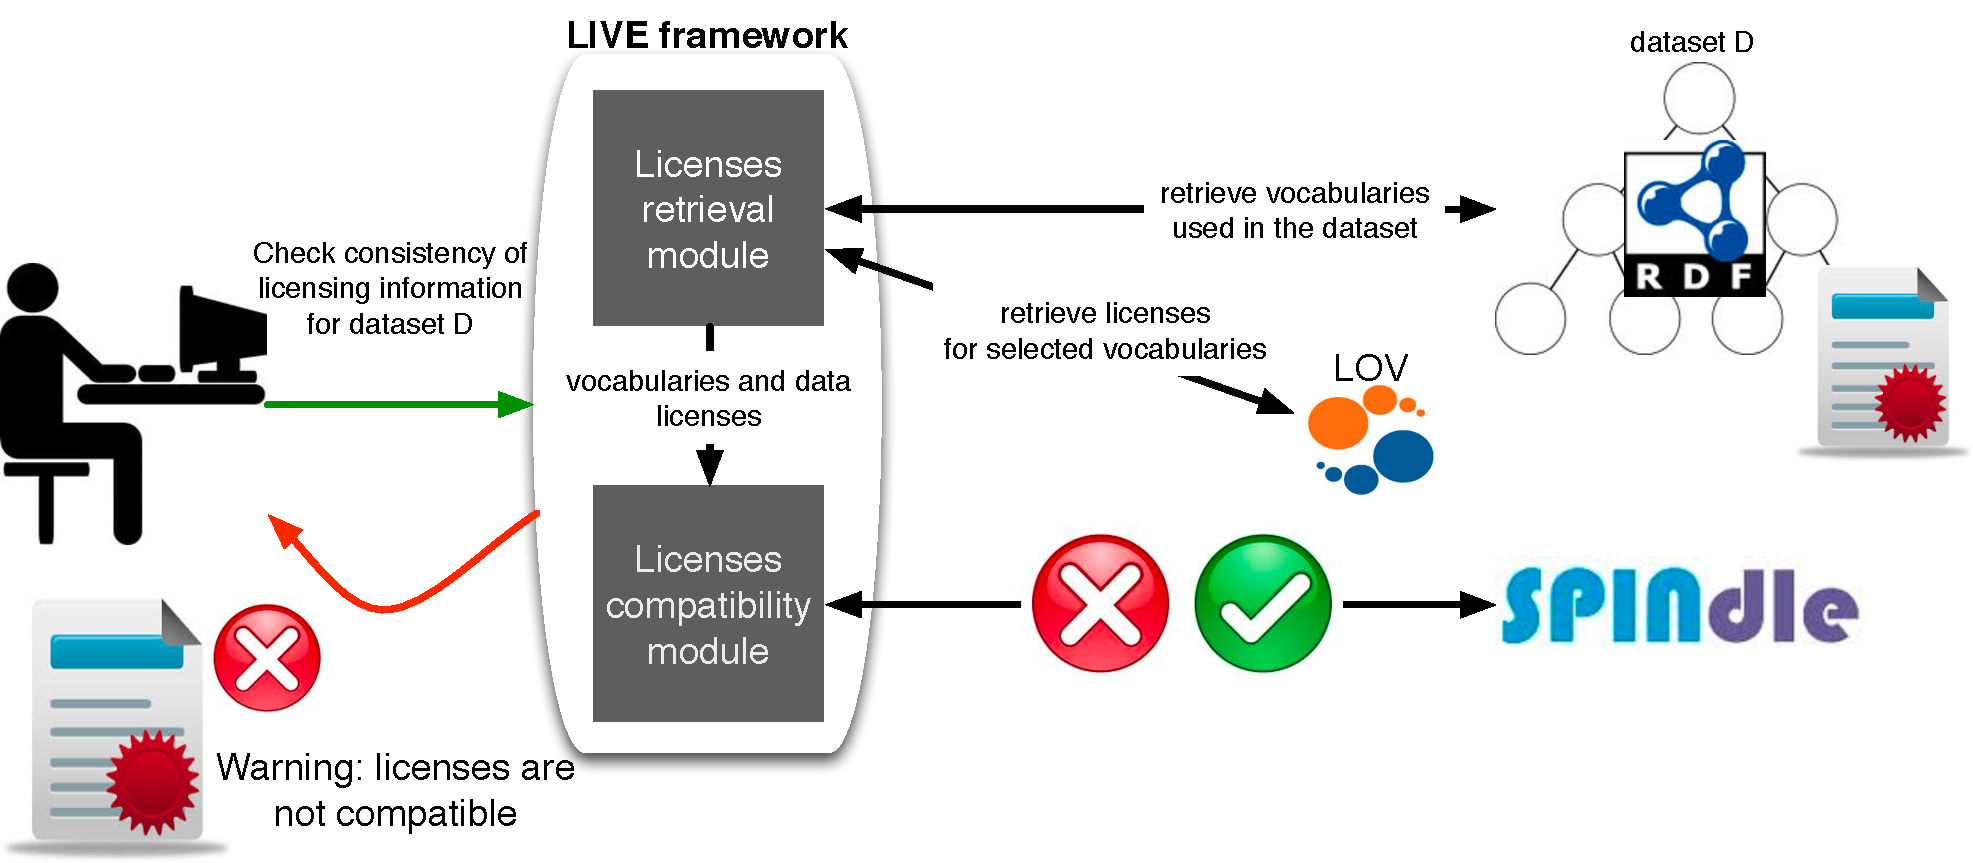
\includegraphics[width=12.0cm]{img/live-framework.pdf}
\caption{LIVE framework architecture.}
\label{fig:framework}
\end{figure}


\subsection{licensing information from vocabularies and datasets.}
Two use-cases are taken into account: a SPARQL endpoint, or a VoID file in Turtle syntax. 
In the first use case, the tool retrieves the named graphs present in the repository, and then the user is asked to select the URI of the graph that needs to be checked. Having that information, a SPARQL query is triggered, looking for entities declared as \texttt{owl:Ontology}, \texttt{voaf:Vocabulary} or object  of the \texttt{void:vocabulary} property. The final step is to look up the LOV catalogue to check whether they declare any license. There are two options for checking the license: \textit{(i)} a \textit{``strict checking'' } where the \texttt{FILTER} clause contains exactly the namespace of the submitted vocabulary, or \textit{(ii)} a \textit{``domain checking''}, where only the domain of the vocabulary is used in the \texttt{FILTER} clause. This latter option is recommended in case only one vocabulary has to be checked for the license. 
%
In the second use case, the module parses a VoID file using a N3 parser for Javascript\footnote{\url{https://github.com/RubenVerborgh/N3.js}}, and then collects the declared vocabularies in the file, querying again LOV\footnote{Since LOV endpoint does not support the JSON format in the results, we have uploaded the data in \url{eventmedia.eurecom.fr/sparql}.} to check their licensing information. 
%
When the URIs of the licenses associated to the vocabularies and the dataset are retrieved, the module retrieves the machine-readable description of the licenses in the dataset of licenses~\cite{CabrioESWC2014}. More specifically, such dataset is composed by 37 licenses, comprising all the licenses adopted to certify data in the Linked Data cloud (as all the Creative Commons licenses\footnote{\url{http://creativecommons.org/licenses/}}), software licenses (as Mozilla Public License\footnote{\url{http://www.mozilla.org/MPL/2.0/}} and Microsoft License\footnote{\url{http://referencesource.microsoft.com/referencesourcelicensing.aspx}}), and additional licenses for other material on the Web (as the UK Open Government license, and the New Free Documentation License\footnote{\url{http://www.gnu.org/copyleft/fdl.html}}). The dataset provides the licenses in RDF using the Turtle syntax, however Creative Commons licenses are also available in XML/RDF format on the CC website\footnote{For instance, Creative Commons Attribution 4.0 license is available at \url{http://creativecommons.org/licenses/by/4.0/rdf}}.

\subsection{Licenses compatibility verification.}
The logic proposed in~\cite{DBLP:conf/semweb/GovernatoriRVG13} 
and the licenses compatibility verification process has been implemented using SPINdle~\cite{spindle} 
-- a defeasible logic reasoner capable of inferencing defeasible theories with hundredth of thousand rules.

%
\begin{figure}[ht!]
% \begin{wrapfigure}{r}{.5\textwidth}
\centering{
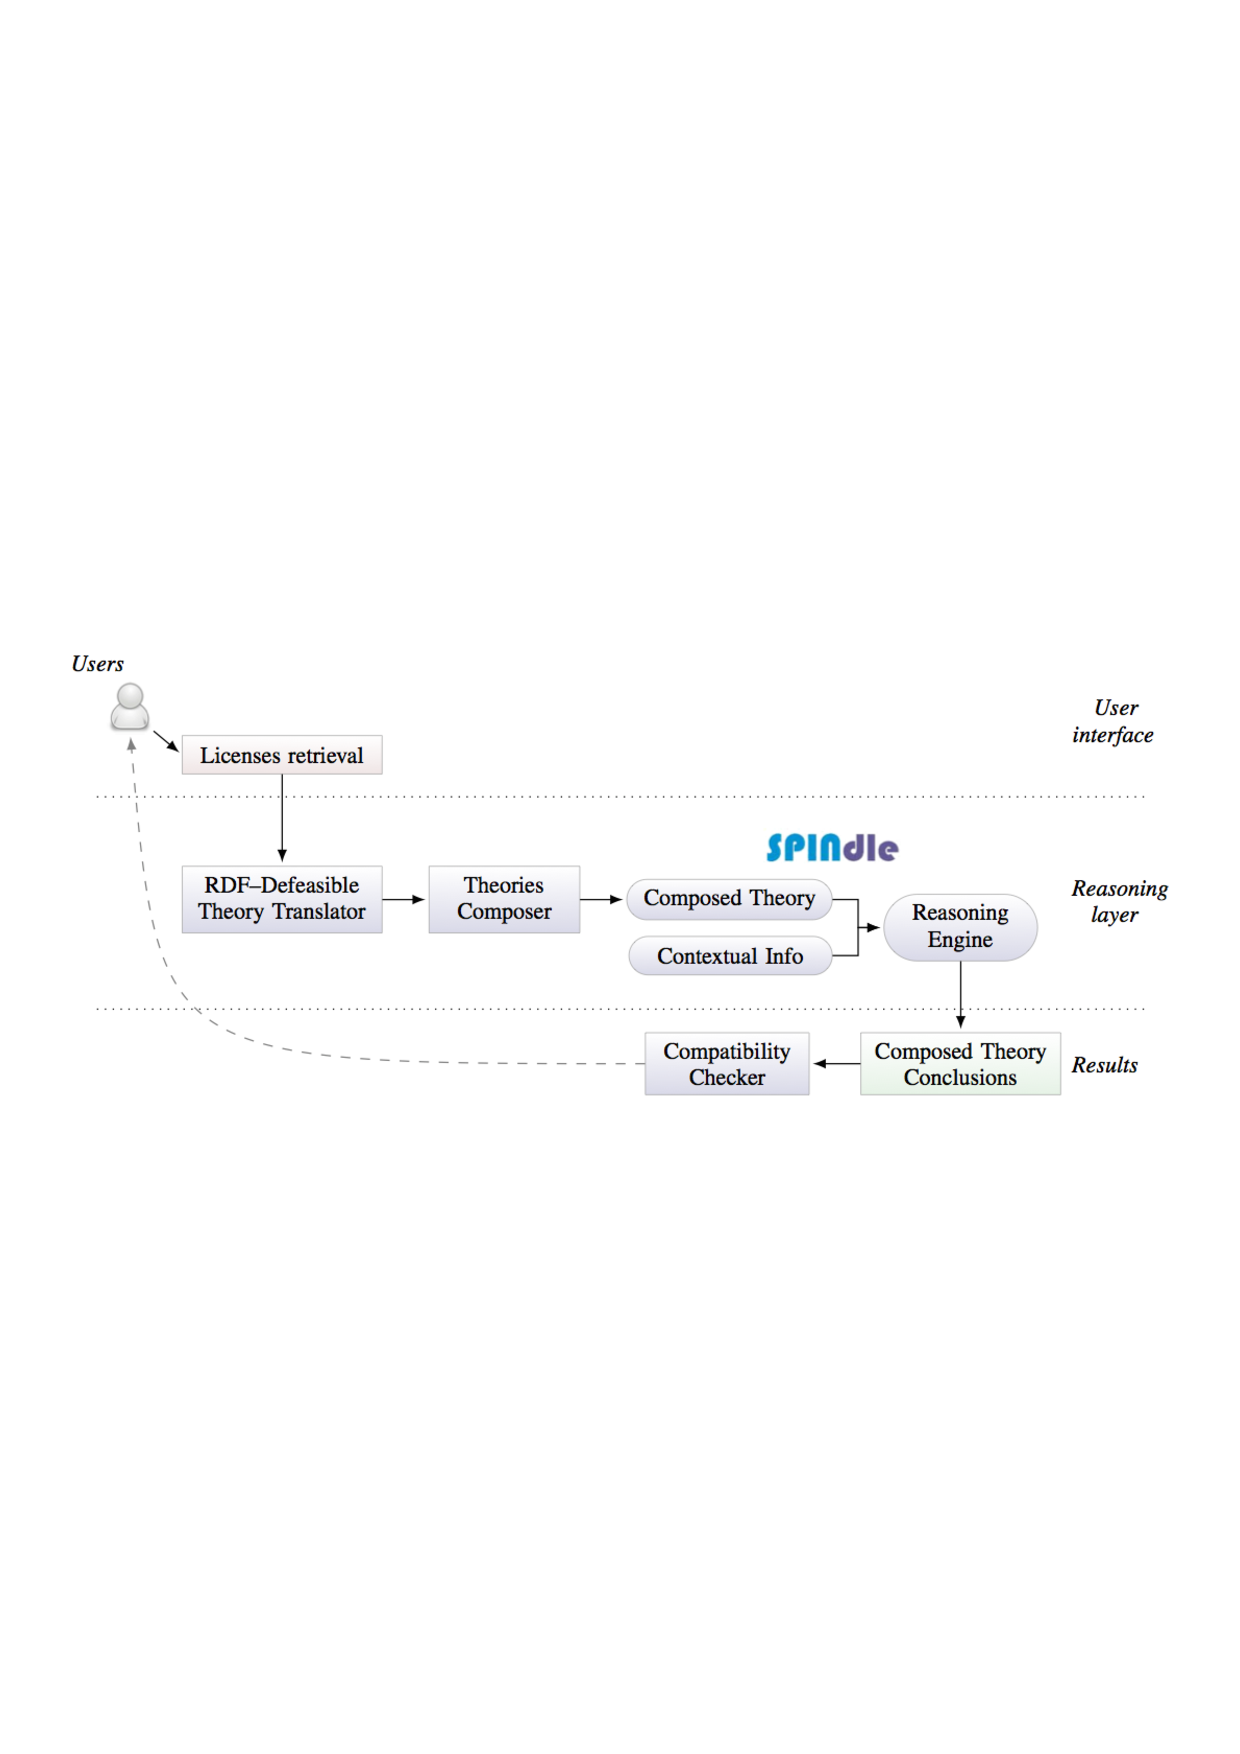
\includegraphics[scale=0.8]{img/composeTheories.pdf}
\caption{Licenses compatibility module.}
\label{figure:theoriesReasoningProcess}
}
\end{figure}
%

As depicted in Figure~\ref{figure:theoriesReasoningProcess},
after receiving queries from users,
the selected licenses (represented using RDF) will be translated into the DFL formalism supported by SPINdle using the \textit{RDF-Defeasible Theory Translator}. 
% If, 
% however,
% more than one license has been selected, % by user,
% then in order to verify the compatibility of different licensing terms, 
% the translated defeasible theories will first be composed into a single defeasible theory~\cite{DBLP:conf/semweb/GovernatoriRVG13} .
That is,
each RDF-triple will be translated into a defeasible rule based on the subsumption relation between the \textit{subject} and \textit{object} of a RDF-triples.
In our case,
we can use the subject and object of the RDF-triples as the antecedent and head of a defeasible rule, respectively.
Besides, 
the translator also supports direct import from the Web and processing of RDF data into SPINdle theories.
%
%the \textit{RDF-Defeasible Theory Translator} will translate the RDF-licenses into the DFL formalism supported by \spindle.

The translated defeasible theories will then be composed into a single defeasible theory based on the logic proposed in~\cite{DBLP:conf/semweb/GovernatoriRVG13},
using the \textit{Theories Composer}.
Afterwards,
the composed theory, 
together with other contextual information (as defined by user),
will be loaded into the SPINdle reasoner to perform a compatibility check before returning the results to the users.

We have evaluated the time performances of the LIVE framework in two steps (Table~\ref{tab:evalTool}).

\begin{table}[ht!]
\centering{
\scriptsize
\begin{tabular}{|l|c|c|c|c|}
\specialrule{1pt}{1pt}{1pt}
 \textbf{Dataset} & \textbf{LicRetrieval(ms)} & \textbf{vocabularies} & \textbf{LicCompatibility(ms)} & \textbf{LIVE(ms)}\\ \hline
  rkb-explorer-dblp & 4 499 &  1 & 0 & 4499\\ \hline
  rkb-explorer-southampton & 14 693 & 1 & 0 & 14 693\\ \hline
  rkb-explorer-eprints & 3 220 & 1 & 0 & 3 220\\ \hline
  rkb-explorer-acm & 3 007 & 1 &  0 & 3 007\\ \hline
  rkb-explorer-wiki & 14 598 & 1 & 0& 14 598\\ \hline
  rkb-explorer-rae2001 & 3 343 & 1 &  0 & 3 343 \\ \hline
  rkb-explorer-citeseer & 2 760 & 1 & 0 & 2 760\\ \hline
  rkb-explorer-newcastle & 3 354 & 1 & 0 & 3 354\\ \hline
  rkb-explorer-kisti & 4 094 & 5 & 6 & 4 100\\ \hline
  270a.info & 13 202 & 48 & 8 & 13 210 \\ \hline
 
\end{tabular}\normalsize
\caption{Evaluation of the LIVE framework.}
\label{tab:evalTool}
}
\end{table}


First, we evaluate the time performances of the licenses compatibility module: it needs about 6ms to compute the compatibility of two licenses. Second, we evaluate time performances (Chrome v. 34) of the whole LIVE framework for the $10$ LOD datasets with the highest number of links towards other LOD datasets, considering both the licenses retrieval module and the licenses compatibility one. The results show that LIVE provides the compatibility evaluation in less than 5 seconds for $7$ of the selected datasets. Time performances of LIVE are mostly affected by the first module while the compatibility module does not produce a significant overhead. For instance, consider Linked Dataspaces\footnote{\url{http://270a.info/}}, a dataset where we retrieve the licensing information in both the dataset and the adopted vocabularies. In this case, LIVE retrieves in $13.20$s $48$ vocabularies, the license for the dataset is CC-BY, and the PDDL license is attached one of the vocabularies\footnote{\url{http://purl.org/linked-data/cube}}. The time for verifying the compatibility is $8$ms, leading to a total of $13.208$s.

\subsection{Future perspectives}
We have introduced the LIVE framework for licenses compatibility. The goal of the framework is to verify the compatibility of the licenses associated to the vocabularies exploited to create a RDF dataset and the license associated to the dataset itself. Several points have to be taken into account as future work. More precisely, in the present paper we consider vocabularies as data but this is not the only possible interpretation. For instance, we may see vocabularies as a kind of compiler, such that, after the creation of the dataset then the external vocabularies are no more used. In this case, what is a suitable way of defining a compatibility verification? We will investigate this issue as well as we will evaluate the usability of the online LIVE tool to subsequently improve the user interface.


\section{Conclusion}
Tell the reader the ``take-away-message'' of this chapter.



\clearpage




\chapter{Conclusions and Future Perspectives}
\label{ch:conc}
\begin{flushright}
\textit{``How do we know that Semantic Web technologies were actually better here, \\as opposed to being what the developers found most familiar?''} \\ (D. Karger)\footnote{\url{http://goo.gl/hQQ3h5}}
\end{flushright}


\section{Conclusions}
\label{sec:final}
%Write here summary of all the work in this document w.r.t the three parts.

This thesis is focused on the challenges of publishing geodata on the Web and a more generic approach to visualize data as Linked Data target to lay-users. The former considers the diversity of different formats used to publish legacy geospatial data, the different projections (or Coordinate Reference Systems) and the representation of complex geometries. The latter approach is different from the state-of-the-art in visualizations where the complexity of SPARQL and RDF is not sufficiently hidden from the users. A deep analysis of the literature has revealed some limitations in the publication of geospatial data and visualization tools, namely:
\begin{itemize}
\item Limited of complex geometries exposed in structured representation, instead of literals. 
\item The absence of an explicit reference to CRSs in direct georeference data on the Web.
\item Absence of visualization tool targeted to lay users to easily grasp the essence of the underlying data published as LOD.  
\item Many data silos for applications built and published on the Web, lost in many HTML pages.
\item Few tools that provide an integrated environment for publishing raw data into Linked Data, from data modeling until the final step of storing the dataset in an endpoint.
\item The difficulty for publishers to understand and check the compatibility of the licenses between vocabularies and datasets.
  
\end{itemize}

In this thesis, we have provided different vocabularies that all together support the publication of geodata integrating almost all the CRSs, extending the existing vocabularies. The vocabularies have been used to publish the French Administrative Units, with the data compatible with GeoSPARQL standards. Regarding the visualizations, after reviewing visual tools and existing applications on the Web, we have developed an ontology to better expose the data on the Web for better interoperability. We have also proposed a framework for  automatically generating visualizations based on categories detected on datasets published as Linked Data, using predefined high level categories used in Information Visualization taxonomy and mapped with vocabularies. 

\subsection{Review of the Contributions}
%\todo{get inspiration with Boris thesis}
This section reviews the main contributions of this thesis and the solutions to solved some of the open research problems in publishing and consuming data on the Semantic Web:

\begin{itemize}
\item We modelled and implemented of a vocabulary for geometry, topological entities and Coordinate Reference Systems (see Section \ref{sec:geomfeaturevocab}).
\item We have implemented of an API for converting data between different CRSs accessible on the Web (see Section \ref{sec:rest-service}).
\item We have published different projections systems used in France with unique URIs to improve look up and integration in structured geometries on the Web (see Section \re{sec:reqs}).
\item We have contributed in the development of the Datalift platform, an integrated environment to publish raw data on the Web (see Section \ref{sec:toolLD}).
\item We have provided a comparison of triple stores for geodata against the geometries handled (literal or structured) to assess which one to use when publishing geospatial data (see Section \ref{sec:geotps}). 
\item We have published French administrative units available as LOD available at \url{http://data.ign.fr} endpoint, based on the vocabularies developed and implemented. Moreover, we have provided interlinking with relevant existing geospatial datasets (see Section \ref{sec:geofla} and \ref{sec:bdtopo} ).

\item We have published in RDF 15 millions of addresses from Open Street Map France using the location address vocabulary (see Section \ref{sec:bano2rdf}).
\item We have contributed to the \textit{French LOD (FrLOD)} cloud, with more datasets published using the Datalift platform, and covering the French territory (see Section \ref{sec:frenchCloud}).
\item We surveyed and classified applications built on top of Open government portals, and proposed a vocabulary for semantically annotate and improve the discovery of applications contests in Open Data event (see Section \ref{sec:descApps} and Section \ref{sec:dvia}).
\item We have proposed a generic approach for automatically generating visualizations based on predefined categories (see Section \ref{sec:ldvizwiz}).
\item We have implemented and evaluated an approach for determining which properties are suitable to use for an entity, based on the Google Knowledge Panel (see Section \ref{sec:propEntities}).
\item We have developed two innovative applications consuming events and statistical datasets (see Section \ref{sec:confomaton} and Section \ref{sec:perfectSchool}).
\item We have proposed a generic plugin tool that can improve the discovery of applications contests in Open Data events (see Section \ref{sec:contests}).
\item We have also proposed an approach to harmonize prefixes used in different catalogues of vocabulary, with an evaluation based on Linked Open Vocabulary (see Section \ref{sec:prefharmoni}).
\item We have developed new ranking metrics for vocabularies based on Information Content theories and applied in LOV (see Section \ref{sec:vocabranking}).

\item Finally, we have built a more efficient tool for checking license compatibility between vocabularies and datasets (see Section \ref{sec:checker}).
\end{itemize}


\section{Future Perspectives}
\label{sec:future}

In this thesis, we have tackled some open research problems within the context of publishing and consuming open data on the Web but there are still open issues and challenges for future work. We  mention some of the most important from our perspective, based on different aspects related to the workflow of publishing Linked Data, more specifically in the geospatial domain. 

\subsection{Opportunities and Challenges for IGN-France}
\label{sec:challenges}

%todo: clarify the context of the opportunities?
 The need for interoperable reference geographic data to share and combine georeferenced environmental spatial information is highlighted by the INSPIRE Directive. The INSPIRE Directive \cite{inspire2009} aims to create a European Union (EU) spatial data infrastructure\footnote{\url{ http://inspire.jrc.ec.europa.eu/index.cfm/pageid/48}}. INSPIRE is based on a number of high level common principles, with some of them very closed to the key concepts of Semantic Web goals, and specifically the Linked Data principles. We provide below the correspondence of our contributions mapped to the five goals of INSPIRE:  
\begin{itemize}
\item \textbf{P1}: \textit{Data should be collected only once and kept where it can be maintained most effectively}. The use of good and stable URI policies can help achieve this principle. IGN as a French geospatial dataset provider, is committed to accurate information, and so will be the URIs chosen for the experimental portal.
\item \textbf{P2}: \textit{It should be possible to combine seamless spatial information from different sources across Europe and share it with many users and applications}. This is more or less the goal of the interlinking tasks performed with other datasets on the wild. The models developed and well-documented can ease the conversion by other mapping agencies or institutions of their datasets.  
\item \textbf{P3}:  \textit{It should be possible for information collected at one level/scale to be shared with all levels/scales; detailed for thorough investigations, general for strategic purposes}. One of the drawback of the models proposed is that they don't currently admit many geometries attached to a feature. This will certainly be one of the extension foreseen for the models. However, the precise classifications for the features is a starter to fulfill this principle.
\item \textbf{P4}: \textit{Geographic information needed for good governance at all levels should be readily and transparently available}. Publishing \url{data.ign.fr} is one of the objective to have also data both in human and machine readable manner using semantic concepts and technologies.
\item \textbf{P5}: \textit{Easy to find what geographic information is available, how it can be used to meet a particular need, and under which conditions it can be acquired and used.} Publishing data on the web contribute \textit{per se} in leveraging their discovery and integration. Moreover, an explicit license attached to datasets published help achieving this principle.
\end{itemize}
For geographic data producers, the benefit of publishing their data on the Web according to Linked Data  (LD) principles is twofold:
\begin{enumerate}
\item First, their data are interoperable with other published datasets and they can be referenced by external resources and used as spatial reference data, which would not have been straightforward when published according to spatial data infrastructures (SDI) standards.
\item Second, the use of Semantic Web technologies can help addressing interoperability issues which are not solved yet by geographic information standards. 
\end{enumerate}
 
Moreover, the French national mapping agency (IGN) has different types of license policies for accessing data from their professional portal\footnote{\url{http://professionnels.ign.fr/}}  (e.g., research purpose, commercial use, access on demand, etc.), with some of them not necessary ``open'' or free to access: (e.g., BD TOPO\circledR). Although there is a clear understanding of the benefits of publishing and interconnecting data on the Web, ongoing investigations on how to combine licenses on datasets are under consideration at IGN. Two solutions are under investigation: 
%(i) different license policies attached to datasets and (ii) the use of a security access mechanism on top of the datasets granting access based on a predetermined configuration on named graphs and resources. 
\begin{enumerate}
\item Different license policies attached to given datasets: Here the attached license is given directly when published. So for example, if it is an open license, the endpoint is publicly available to be queried without any restriction.
\item The use of a security access mechanism on top of the datasets granting access according to a predetermined configuration list of named graphs, resources and operations allowed. This solution goes along with the work of Rotolo et al.\cite{rotolo2013deontic}, where even if there is an endpoint, a module for configuring the types of queries to perform and access policies have to be defined for subsets with special care to take into account compositions of licenses in the results.
\end{enumerate}
According to Linked Data principles URIs should remain stable, even if administrative units change or disappear. This implies adapting the data vocabulary in order to handle data versioning and time scale evolution of the data. This issue will be addressed in our future work, as we are working on releasing a spatio-temporal dataset describing the evolution of communes since the French Revolution. Another issue deals with the automation of the whole publication process, from traditional geographic data to fully interconnected RDF data.
The last issue deals with the use of multiple geometries for describing a geographic feature: geometries with different levels of detail, different CRS, different representational choices. This has been superficially addressed in our use case with the use of both polygons and points for representing respectively the surface and the centroid of departments, but should be further investigated for both query answering and map design purposes.


\subsection{Generic Visualizations on Linked Data}
We plan to use a more exhaustive set of vocabularies in our generic queries for detecting those categories, plugging into directly the wizard to the LOV catalogue. The aggregation properties can be extended to take other semantic relations (e.g: \texttt{skos:exactMatch}) into account. Additionally, we plan to make an evaluation of the prototype and compare it to related tools such as the ones aiming to build profiles of datasets. We also need to quantify when a category is ``important'' within a dataset. For example, is it enough for a dataset to be classified GEODATA with ten triples containing location? From which number of triples could the categories and hence the visualizations be assigned? These issues can further be investigated to find the best trade-off.  Another drawback of our work on visualizations is the lack of user evaluation, with experiments to understand users' needs, focusing more on the semantic aspects than just the exploration ones (webby-interface). A natural follow-up is use these evaluations and re-adapt the applications/visualizations based on the results. 
 
\subsection{Vocabularies and LOV}
\label{sec:nextSteps}
Work on the harmonization of prefixes can be extended in several directions. Sticking to the two services we have studied and already contributed to harmonize, the possible next steps would be to automate as far as possible the tasks that have been made semi-automatically so far:
\begin{itemize}
\item \emph{i)} developing a unique interface for submitting namespaces and prefixes to both services;
\item \emph{ii)} bridging the LOV back-office and the prefix-cc database using both services API in order to publish a list of common recommended prefixes. 
\end{itemize}  The latter goes beyond the limited framework of the two original services since such a list could be consolidated and endorsed by the main actors in vocabulary publication and management, and recommended for use in linked data applications. This could be picked up by the upcoming W3C Vocabulary Management Working Group as part of the new Data Activity\footnote{\url{http://www.w3.org/2013/05/odbp-charter.html}}.

%\todo{here is the perspective for ranking voabs} \\
\paragraph{}
 As per ranking vocabularies, we aim to take into account the equivalence axioms (between classes and properties) when computing the Information Content, and more generally, all sort of semantic relationships between terms. Also, we plan to compare our ranking model with other ranking approaches such as graph-based ones (e.g., pagerank). Another future direction is to investigate the dependency ranking between vocabularies, by focusing on a specific type of ``inlinks'' (i.e. extensions, generalizations) and study how they affect the information content (PIC) metrics.


\paragraph{}
We have made the assumption in this thesis that access to data was either by  querying a SPARQL endpoint, or by browsing or by downloading the dumps. Recently, a new way of accessing the data on the Web is emerging: through triple pattern fragments\footnote{\url{http://linkeddatafragments.org/}}. Linked Data Fragments \cite{verborgh2014ldf} aims at exploring endpoints with simple fragments to solve queries at the client side with server data.
Servers can offer data at low processing cost in a way that enables client-side querying, thus, moving intelligence from the server to the client. One possible direction of study could be to use client-side concept for evaluating endpoints consuming only structured geometries versus literal for real-world applications. Finally, triple fragment concepts can be applied also to detect also patterns for visualization in different endpoints.
 
% \todo{discuss here if it could be wise to use Linked Data Fragments... maybe as future work?}
\todo{add a paragraph about vision future work}

 


\appendix
\chapter{Installation instructions for the JavaScript plugin}
\label{ch:appendixA}

The system consists of three components, each having their own code repository:
\begin{itemize}
\item Admin-interface: This is the interface that event organizers use to create new events and to get the embed code for embedding the event on their own website. It is available at \url{https://github.com/EurecomApps4Eu/admin-interface}. 	
\item REST-interface: This interface provides a RESTful service for events and applications, available at \url{https://github.com/EurecomApps4Eu/rest-interface} 
\item Embeddable script at \url{https://github.com/EurecomApps4Eu/event-website}. This repository contains the code that is embedded on the event organizer's own website. It will fetch the event and application information from the REST-interface, and then display the information directly on the event organizers webpage.
\end{itemize}

The three different components can be installed on different computers, if needed. REST-interface requires Node.js and MongoDB to be installed, whereas Admin-interface and Event-website produces static files (when running the build task) that can be hosted on any web server that is capable of serving static files.

\section{Installing and configuring the REST-interface}
\begin{verbatim}
1.	Clone the repository
2.	Install dependencies by running the command "npm install"
3.	Configure the system by editing "config.js"-file
4.	Start the service by running "node app.js {PORT}", and replace {PORT} 
with the port you want to run the application in (typically port 80 for HTTP)

\end{verbatim}

\section{Installing and configuring the Admin-interface}
\begin{verbatim}
1.	Clone the repository
2.	Install Node dependencies by running the command "npm install"
3.	Install Bower dependencies by running the command "bower install" 
(if bower is not installed run "npm install bower -g")
4.	Configure the system by editing file "app/scripts/app.js". 
Look for appSettings-part in the file.
5.	Build the system with command "grunt build" 
(if grunt is not installed, run "npm install grunt -g").
This will produce static HTML/CSS/JS-files that can be hosted on any web server.
\end{verbatim}

\section{Installing and configuring the Event-website}
\begin{verbatim}
1.	Clone the repository
2.	Install Node dependencies by running the command "npm install"
3.	Install Bower dependencies by running the command "bower install" 
(if bower is not installed run "npm install bower -g")
4.	Configure the system by editing file "config.js"
5.	Build static HTML/CSS/JS-files by running "grunt all"

\end{verbatim}


%\include{Appendix2}
%\include{Appendix3}

%

\bibliographystyle{plain}
%\bibliographystyle{abbrv}
\bibliography{thesis}
\nocite{*}
\printnomenclature

%\chapter*{}
%\chaptermark{}
%\section*{}
%\sectionmark{}
%\vspace{-15ex}
%\appendix
\end{document}
 
